%!TEX TS-program = xelatex
%!TEX encoding = UTF-8 Unicode

\documentclass{harvard-thesis}
\usepackage[norsk]{babel}
\usepackage{parskip}
\usepackage[norsk]{inputenc}
\usepackage{hyperref}
\usepackage{url}
\usepackage{dirtytalk}

\usepackage{pdfpages}
%\usepackage[section]{placeins}
%\usepackage[subsection]{placeins}
\usepackage{float}
\usepackage{babelbib}
%\usepackage[authordate]{biblatex-chicago}
%\DeclareFieldFormat[article]{title}{\mkbibquote{#1}} % make article titles in quotes
%\DeclareFieldFormat[thesis]{title}{\mkbibemph{#1}} % make theses italics
%\addbibresource{references}
\usepackage{lscape}
\usepackage{longtable}
\usepackage{tabularx}
\usepackage{listings}
\usepackage{color}

\usepackage{minted}
\usepackage{blindtext}
 
\begin{document}

% the front matter
% some details about the thesis
\title{Millum Procurement Varetelling}

\author{Gruppe 16}

% about the degree
\field{i BAO300 - Bachelorprosjekt}
\degreeyear{2020 - 2020}

% about the university
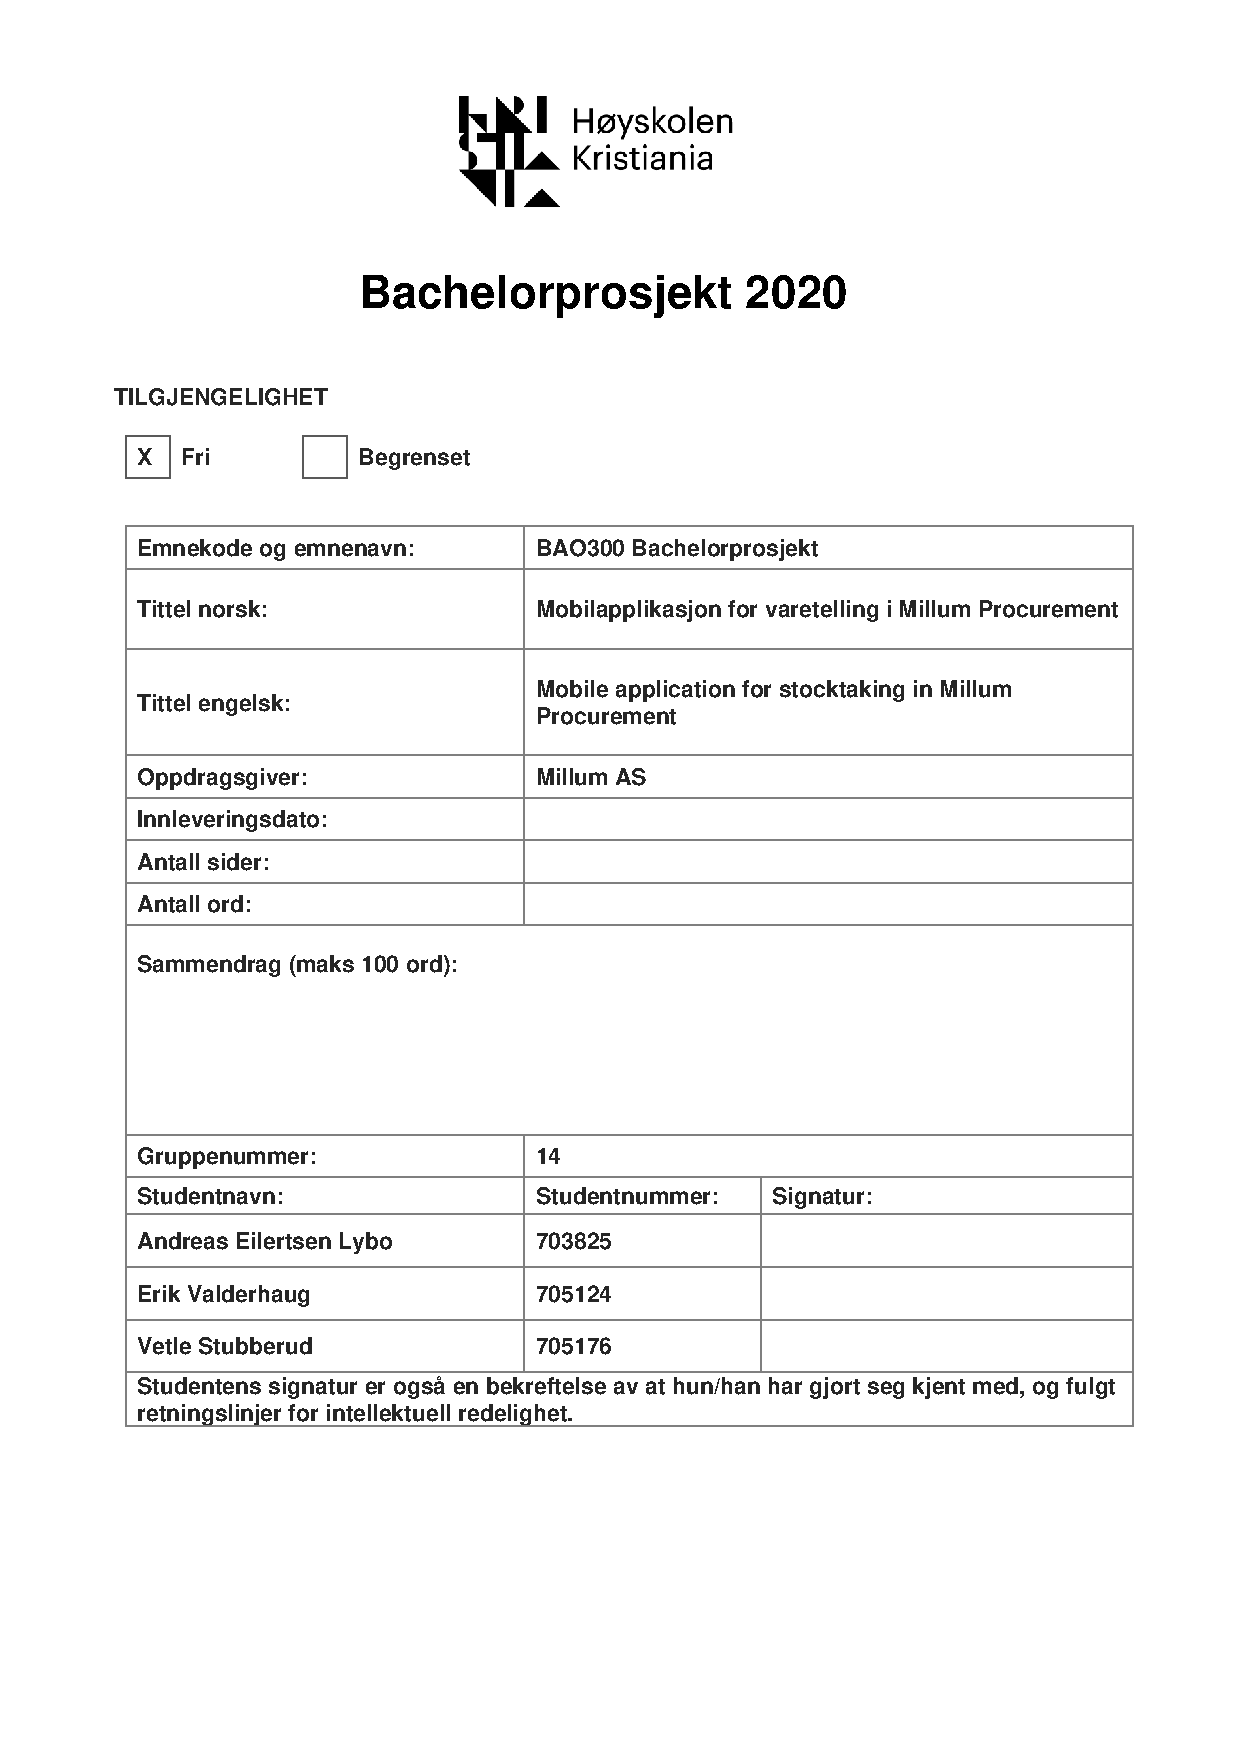
\includepdf[pages=-]{figures/Forside.pdf}
\setcounter{tocdepth}{2}
\tableofcontents
%\acknowledgments
\listoffigures
\chapter{\color{Millum}\textbf{Dokumentets struktur}}
Dokumentet er skrevet kort og konkret. Utdypninger finnes i egne vedlegg. Hvert vedlegg finnes avslutningsvis i oppgaven og referanser er lagt ved der det er naturlig. Referansene fungerer som hyperlenker til kapittelet om \textbf{\nameref{chap:vedlegg}}.\newline

Oppgaven er skrevet med mange tekniske begreper og domeneord for bransjen vi utviklet løsningen for. Forklaringer på begreper er lagt ved der det er naturlig, og i egen begrepsliste \textbf{(REFERANSE BEGREPSLISTE)}


%\abstractpage
%\authorlist


\onehalfspacing

% include each chapter...
\include{chapters/innledning}
\chapter{\color{Millum}\textbf{Prosess og metode}}
\newthought I dette kapittelet går vi nærmere inn på prosesser og metoder vi har valgt, samt gjør vi rede for og drøfter vår prosjektplanlegging og arbeidsprosess.

\section{\textbf{Forskningsmetodikk}}

Samtidig som vi gjennomførte bachelorprosjektet hadde vi emnet ''Undersøkelsesmetoder''. I dette var det flere læringsmål som omfatter hele prosessen ved å gjennomføre en undersøkelse for et IT-prosjekt og begrunne valg av metode ut fra en faglig gitt problemstilling. Vår eksamensinnlevering \textbf{(ref undersøk.met eksamen)} ble gjennomført med hensikt å kunne bruke det vi lærte i vårt bachelorprosjekt. Resultatet av oppgaven er en rapport med problemstillingen:

\textit{''Hvordan redusere kostnad og tidsbruk i forbindelse med varetellingsrutiner?''}


Vår valgte metode for datainnsamling har vært en spørreundersøkelse \cite{oates2006researching} (Oates, s. 93). En stor fordel med spørreundersøkelser er at vi når ut til målgruppen raskt. Vi har derimot ingen forutsetningen til å vite spesifikt om hvilke kunder som gjennomførte spørreundersøkelsen. Terskelen for et individ til å gjennomføre en spørreundersøkelse er også langt lavere enn det å eksempelvis gjøre et én-til-én intervju. I tillegg hadde vi også muligheten til å innhente både kvalitative og kvantitative data.

\subsubsection{\textbf{Kvalitative og kvantitative data}}

Vi skiller mellom kvantitative og kvalitative data. “Kvantitative data” betyr data, eller bevis, basert på tall (Oates, s. 245). Kvalitative data inkluderer all ikke-numerisk data. Dette vil være for eksempel ord, bilder og lyd. (Oates, side 267). Ofte vil man samle inn kvantitative data når man gjennomfører eksperimenter og spørreundersøkelser. Kvalitative data kommer som oftest fra intervjuer, observasjoner, dokumenter og video.
For de kvantitative dataene er det statistiske metoder som danner fundamentet for analyse. Formålet med statistiske metoder er å skaffe kunnskap om en større mengde enheter (individer eller objekter).

For vår datainnsamling støter vi på både kvalitative og kvantitative data.

\begin{figure}[H] 
    \centering
    \includegraphics[width=\textwidth]{figures/Prosess-og-metode/spørreund.PNG}
    \caption{Oversikt over hele spørreundersøkelsen}
\end{figure}

Før vi sendte spørreundersøkelsen fikk vi tekstskribenten hos oppdragsgiver til å gjennomføre og gi tilbakemeldinger på undersøkelsen for å kvalitetssikre at vi oppnådde de målene vi hadde satt for undersøkelsen.

Vi planla videre å gjennomføre brukertester med flere av kundene, men fikk dessverre ikke mulighet til dette grunnet pandemien. Vi kommer tilbake til utfordringene rundt dette i \textbf{\ref{Andre_utfordringer}}.

Hva vi lærte av forskningen og hvordan vi har knyttet det opp mot prosjektet vårt kommer vi tilbake til i \textbf{\ref{Kartlegging_behov}}.

\section{\textbf{Prosjektmetodikk}}
I dette kapittelet skal vi gjøre rede for og drøfte vår prosjektplanlegging og arbeidsprosess.

\section{\textbf{Moderne IT prosjekter}}
Det er en rekke ulike måter å sette opp et IT prosjekt på. Vi deler opp typer prosjekt i to hovedgrupper. Agile og Plan driven. Plan driven er prosjekter med strenge seremonielle krav til struktur og dokumentasjon som for eksempel Waterfall. Agile derimot er prosjekter som setter inkrementelle og iterative prosesser fremfor seremonielle strukturer. I dag følger de fleste større IT selskaper en Agile filosofi med ulike implementasjons varianter. SCRUM, Agile-Prince2, SCRUM-Devops, Agile-Lean er alle ulike implementasjoner av en Agile filosofi med ulike rammeverk brukt for implementasjon. Plan driven og Agile prosjekter eksisterer på to ulike akser hvor prosjekter er mindre eller mer Agile/Plan Driven. De fleste prosjekter vil ligge et sted mellom Plan Driven og Agile. Dvs at de inneholder momenter fra begge filosofier. 


\subsection{\textbf{Plan Driven}}
Plan driven management er en eldre og mye brukt prosjektledelsestil. 

 ``\textit{A style of development that attempts to plan for and anticipate up front all of the features a user might want in the end product and to determine how best to build those features. The work plan is based on execution of a sequential set of work-specific phase}s`` (2020. Plan-Driven Process. Innolution LLC).  

Fordelen med en plandrevet tilnærming er at prosjektet ofte blir lettere å styre. Endringer, hindringer og mål dokumenteres godt for å forebygge eventuell risiko. Problemet med denne tilnærmingen er derimot at om det oppstår uforutsette hendelser som ikke er en del av risikoplanen kan det være vanskelig å tilrettelegge prosjektet. Prosjekter har derfor en større risiko for avbrudd dersom forandring må foretas. Dette er en av hovedgrunnen til at mange IT-selskaper har valgt å gå bort ifra en streng plan driven tilnærmingen. IT-prosjekter har en tendens til å inneha en stor grad av forandring ettersom brukerens ønsker og utviklingskriteriene er i konstant forandring. Dette betyr dog ikke at moderne IT-prosjekter ikke innebærer planlegging. Alle prosjekter trenger en overordnet struktur for å kunne fungere. 

I et plandrevet prosjekt legges det opp til en stor sluttlansering av produktet. En klassisk form for prosjektstyringsstil heter Waterfall. Dette er prosjekter som følger en overordnet sekvensiell struktur:
\begin{itemize}
    \item \textbf{Requirements}. Krav til spesifikasjon.
    \item \textbf{Design}. Utforming av produktet.
    \item \textbf{Implementation}. Arkitektur og implementasjon.
    \item \textbf{Verification}. Bekreftelse på at kravene er nådd.
    \item \textbf{Maintenance}. Videre vedlikehold av produktet.
\end{itemize}
Hvert enkelt steg må fullføres før prosjektet kan fortsette til neste steg.    

\subsection{\textbf{Agile}}
I 2001 møttes 17 utviklere på et resort i Utah, USA for å diskutere en rekke utviklingsmetoder som nylig hadde dukket opp. Resultatet av møtet var et manifest som kalles \textit{The Agile Manifesto}. I dette manifestet legges det frem en rekke prinsipper som danner grunnlaget for smidig utvikling.

\textit{We are uncovering better ways of developing software by doing it and helping others do it. Through this work we have come to value:}
\begin{itemize}
    \item \textbf{Individuals and interactions} over processes and tools
    \item \textbf{Working software} over comprehensive documentation
    \item \textbf{Customer collaboration} over contract negotiation
    \item \textbf{Responding to change} over following a plan
\end{itemize}

\subsubsection{\textbf{The Agile Manifesto}}
Dette manifestet sammen med en rekke bøker og Agile alliances \textit{Agile glossary}
dannet grunnlaget for smidig prosjektutvikling. 

Agile er en utviklingsmodell som inneholder ulike tilnærminger til programvareutvikling hvor løsninger og krav utarbeides gjennom samhandling, selvorganisering og kryssfunksjonelle lag. Agiles metodikk er alltid rettet direkte mot sluttbrukerens ønsker. Agile omhandler adaptiv planlegging, evolusjonær utvikling, tidlig leveranse av produkt og kontinuerlig forbedring.
 
Istedenfor å legge alt i en stor lansering jobber et smidig team i mindre inkrementelle lanseringer. Forventninger, planer og resultater er evaluert kontinuerlig for å gi teamet en naturlig måte å justere seg til forandring. Selv om det hovedsakelig er prosjektleder og produkteier som prioriterer det arbeidet som skal leveres er det opp til gruppen selv hvordan oppgavene burde løses.
 
Agile er ikke definert av et sett seremonier eller spesifikke utviklingsmetoder, men er heller en tankegang eller tilnærming til planlegging og prosjektløsning hvor korte sykluser for tilbakemeldinger og kontinuerlig forbedring står i sentrum. Det originale Agile manifestet beskrev ikke nyere smidig praksis som x antall ukers sykluser eller et ideelt team størrelse, men la heller frem prinsipper.
 

\section{\textbf{Scrum}}
Scrum er et rammeverk som hjelper team å jobbe sammen. Scrum legger i likhet med Agile vekt på læring gjennom erfaring. Det vil si iterasjon og autonomi for hvert enkelt teammedlem og oppfordrer til refleksjon for kontinuerlig forbedring. 

Selv om Scrum hovedsakelig blir brukt av utviklingsteam kan prinsippene og lærdommen benyttes i all slags lagsamarbeid. Dette er en av grunnen til at Scrum har blitt et populært rammeverk. Scrum blir ofte beskrevet som et smidig prosjektstyringsrammeverk, og beskriver et sett av møter, verktøy og roller som henger sammen for å hjelpe team å strukturere og gjennomføre arbeid.

Agile og Scrum blir ofte sett på i sammenheng fordi Scrum i likhet med Agile sentreres rundt kontinuerlig forbedring. Forskjellen ligger i at Scrum er et rammeverk for å få arbeid gjort, mens Agile er et mer overodnet \textit{tankesett}. Det er ofte vanskelige å få Agiles tankegang ut i praksis fordi det trengs dedikasjon fra hele teamet for å forandre deres tankegang. Man kan derimot bruke et rammeverk som Scrum for hjelpe til å danne et grunnlag for smidig tenkning og for å øve på å bygge smidige prinsipper inn i kommunikasjon og arbeid.

\subsection{\textbf{Faser og prosess}}
Rammeverket Scrum tar utgangspunkt i at teamet ikke kan vite alt i starten av prosjektet og at prosjektet naturlig vil utvikle seg. Scrum er strukturert til å hjelpe team til å naturlig tilpasse seg forandring. Derfor innehar Scrum korte, definerte sykluser for å gi teamet mulighet til å kontinuerlig lære og forbedre seg.

\subsubsection{\textbf{Sprint}}
En sprint er Scrums iterative fikserte tidsramme hvor et “ferdig” produkt av høyest mulig verdi produseres. Teamet spesifiserer en tidsramme på som oftest 2-4 uker hvor en rekke mål blir definert som skal jobbes på og nøye gjennomgås i løpet av sprinten. Hvis en gjennomgang viser et avvik i produktet justeres produktet så fort som mulig for å forhindre videre avvik. Alt arbeid som er gjort og skal gjøres loggføres i en produkt backlog som videre brukes til å estimere ferdigstilling av produktet.

\subsubsection{\textbf{Produkt Backlog}}
En produkt backlog er en liste av gjøremål som trengs i løpet av prosjektets levetid. Elementene i listen kan være tekniske løsninger, krav eller mer brukerorienterte krav i form av brukerhistorier, heretter kalt "User Stories". User stories er korte konsise beskrivelser fortalt fra brukerens perspektiv. Et eksempel på en user story i vår løsning er: “Som bruker av applikasjonen ønsker jeg å kunne logge inn i applikasjonen slik at jeg får tilgang til mine varetellinger”. Eieren av en produkt backlogen er produkteieren. Scrum master, Scrum team og interessenter bidrar til å ferdigstille produkt backlogen. 

Forskjellen på en Scrum backlog og en enkel gjøremålsliste ligger i at et element i Scrum backlog alltid rettes mot, arrangeres og prioriteres mot sluttbruker, i tillegg til at alle elementer i en Scrum backlog estimeres. 


\subsubsection{\textbf{Sprint Backlog}}
En Sprint backlog er en backlog med et undersett av elementer tatt fra prosjektbacklogen som skal gjennomføres i løpet av en Sprint. Sprintbacklogen ligner produkt backlogen i oppbygning.

\subsubsection{\textbf{Produkteier}}
Produkteier bestemmer og definerer produktet som skal utvikles til enhver tid. I samarbeid med utviklingsteamet defineres oppgaven og dens akseptansekriterier. I vårt prosjekt har produkteier vært en komite av scrum master, produkteier og systemarkitekt for handelsplattformen vi utvikler mot, og de har vært ansvarlig for å definere brukerbehov i form av user stories.

En produkteier kan kun være et individ, selv om dette individet kan være representert gjennom en komite. Jobben deres innebærer:
\begin{itemize}
    \item Opprettholde produktbacklogen
    \item Prioritere i produktbacklogen
    \item Sørge for at elementer i produktbacklogen er forståelig for utviklingsteamet
\end{itemize}

I vårt tilfelle har produkteier vært ppdragsgivers eksisterende produkteier.

\subsubsection{\textbf{Scrum Master}}
Scrum master kan på mange måter sammenlignes med en prosjektleder og coach. Ansvaret denne personer har er å sørge for at teamet forstår oppgavene i backlogen, sørge for fremdrift i prosjektet og være en støttespiller for utviklingsteamet samt holde unødvendig støy borte fra teamet. Dette kan for eksempel være kunder som maser om budsjett som kan forstyrre teamet i sine daglige  gjøremål. Denne personen skal også være ansvarlig for å fasilitere sprintrelaterte møter som daglig stand up, sprint review, sprint retrospective osv. Selv om man gjerne sammenligner Scrum Master med en prosjektleder har ikke denne personen tradisjonell beslutningsmakt og skal heller ikke hindre teamet i å komme frem til løsninger sammen.

\subsubsection{\textbf{Utviklingsteamet}}
Utviklingsteamet er ansvarlig for å implementere elementer i produkt backlogen.

\subsubsection{\textbf{Daglig stand up}}
Daglig stand up er et daglig møte oftest holdt på starten av dagen hvor de neste 24 timene med arbeid planlegges og de forrige 24 timene oppsummeres. Hvert enkelt gruppemedlem bruker noen få minutter til å snakke om hva de har arbeidet med og hva de skal arbeide med videre. Det estimeres tidsbruk ofte gjennom en burndown graf og funksjonalitet diskuteres. Fokuset her ligger mye på utfordringer som teamet kan bidra med å løse. I mange sporter har laget en strategisk samling før, under eller etter en kamp. Samlingen gjør laget informert, synkronisert og kalibrert gjennom kampen. Daglig stand up er Scrums måte å samle laget før en kamp. Den gir teamet en følelse av samhold.

\subsection{\textbf{Fordeler med SCRUM}}

\subsubsection{\textbf{Smidig forandring}}
Med korte planleggingsfaser er det lett å legge til rette for forandring uansett hvor eller når i prosjektet det gjøres. I hver Sprint gjennomgåes produktets backlog og nye mål settes. Produkteier har også mulighet til å forandre på deres ønsker og prioriteringer gjennom hele prosjektet. 

\subsubsection{\textbf{Tett kommunikasjon med oppdragsgiver}}
Scrum gir kunden mulighet til å ta del i utviklingsprosessen fra start til slutt. Faste sprint review-møter med oppdragsgiver og en produkt backlog gir kontinuerlig kommunikasjon mellom oppdragsgiver og utviklingsteamet. 

\subsubsection{\textbf{Oppfordrer til kommunikasjon innad i teamet}}
Agile fremhever viktigheten av hyppig kommunikasjon og face to face interaksjon. Scrums daglig stand ups gir teamet en god måte å holde seg oppdatert med prosjektets progresjon


\subsection{\textbf{Ulemper med Scrum}}

\subsubsection{\textbf{Mindre konkret planlegging}}
Det kan være vanskelig å fastsette en konkret utgivelsesdato ettersom prosjektet er i konstant endring. Scrum fastsetter en tidsramme for når produktet skal ferdigstilles i stedet for en fastsatt utgivelsesdato. Når tidsfristen er ute leveres produktet i sitt daværende stadie. Dette kan gjør at produktet som leveres ikke alltid blir godt nok ferdigstilt. 

\subsubsection{\textbf{Vanskelig for større team å følge}}
Scrum avhenger av kontinuerlig kommunikasjon innad i teamet. Dette kan være et problem i store utviklingsteam med flere ulike avdelinger. Dette gjør at mye av tiden ofte blir brukt til organisering av prosesser i stedet for produktivitet. 

En løsning på dette som ofte benyttes er å dele inn større prosjekter i flere individuelle team. Hvert enkelt team blir delegert en del av et større prosjekt eller et produkt. Dette gjør det enklere å holde styr på gruppens medlemmer.

Andre større selskaper bruker ``Scrum of scrums`` for å lettere håndtere mindre teams i en stor organisasjon.

\subsubsection{\textbf{Prokrastinering}}
Gjennom arbeid med et større prosjekt er det ofte at selv velmente og hardt arbeidende personer utsetter å arbeide med et prosjekt. 

\section{\textbf{Hvorfor vi valgte Scrum}}
Siden Scrum som rammeverk gir oss fleksibiliteten til å plukke de delene av prosessen som passer oss best, og kvitte oss med de andre ga det gruppen en bedre forutsetning for å møte hindringer underveis i prosessen. Det var i starten av prosjektet usikkerhet rundt oppgaven og måten vi skulle løse oppgaven på. Derfor var det å velge et rammeverk som gir oss stabilitet og mulighet til å effektivt kunne tilpasse oss forandringer i gruppens sammensetning eller fremgang i prosjektet helt sentralt. Vi hadde i tillegg mulighet til å følge arbeidsmetodikken til oppdragsgiver som gjorde det lettere å planlegge møter med interessentene. 

\section{\textbf{Vår bruk av Scrum}}
Siden Andreas kjenner best til oppdragsgiver og handelsportalen Millum leverer var det naturlig at han gikk inn i en rolle som Scrum Master i starten av prosjektet. Det gjorde det lettere å samhandle med oppdragsgiver og sørge for fremgang i starten av prosjektet hvor det var mye usikkerhet. 

Teamet bestemte seg for å følge oppdragsgiver sin lengde på sprintsykluser, som er 2 ukers iterasjoner. Dette er ideelt så teamet både kunne følge Millum sin struktur, men også siden lengden passer fint med tanke på hvor mye tid som går til planlegging og gjennomføring av de ulike møtene.

Vi benyttet oss til dels av daglig stand up, men etterhvert som teamet fikk forståelse for prosjektet var det mindre nødvendig å ha standup hver dag siden vi uansett satt så tett på hverandre. 

I slutten av hver sprint inviterte vi interessenter fra Millum til en gjennomgang av hva vi hadde løst i løpet av sprinten. Det ga oss mulighet til å kontinuerlig få tilbakemelding fra mennesker med mer erfaring og innsikt i markedet vi jobbet mot, men også sørge for at de var oppdatert på progresjonen vi hadde i prosjektet.

Etter Sprint Review satte teamet av tid til refleksjon i form av en Sprint Retrospective. Hensikten var at teamet skulle ha en dedikert arena til å ta opp ting som kanskje ikke var så lett å dele i plenum, og samtidig ta med seg de gode elementene fra sprinten så vi kontinuerlig lærer og utvikler oss som team. Under denne sesjonen fikk alle teammedlemmene utdelt tre post-it lapper hvor man skulle vurdere:

\begin{itemize}
    \item \textbf{Score 1-5 for sprinten}. 1 er dårligst og 5 er beste mulige score.
    \item \textbf{Forbedringspotensiale}. Brukte teamet for lite tid til å forberede presentasjonen til interessenter, eller synes man kanskje at meningene sine ikke ble hørt.
    \item \textbf{Ta med videre}. Hva synes man var bra med sprinten? Hadde man god kommunikasjon, eller klappet man hverandre på ryggen når man leverte god kode?.
\end{itemize}

Hvordan Scrum fungerte for oss i dette prosjektet kommer vi tilbake til i \textbf{\ref{Vurdering_SCRUM}}














\chapter{\color{Millum}\textbf{Tekniske valg}}
\newthought {Som en naturlig del av et IT-prosjekt} er de tekniske valgene grunnlaget for prosjektets fundament. I dette kapittelet drøfter vi valg av programmeringsspråk, rammeverk og arkitektur tilhørende denne prosessen.

\section{\textbf{Programmeringsspråk og rammeverk}}
\begin{figure} 
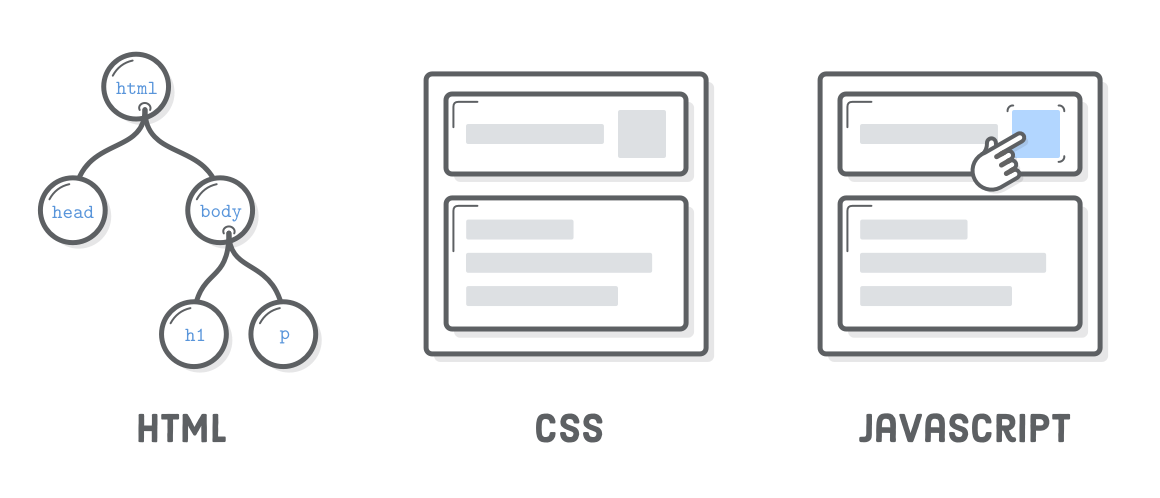
\includegraphics[width=\textwidth]{figures/HTML-CSS-JS.png}
\caption{De tre delene som websider bruker til å samhandle med}
\end{figure}
For å kunne utvikle nettbaserte applikasjoner må man ha kunnskap om HTML, CSS og JavaScript. Denne treenigheten legger grunnlaget for dynamiske, nettbaserte applikasjoner. Tenk på HTML som dokumentet som definerer strukturen til applikasjonen, CSS som den visuelle fremvisningen og JavaScript som definerer applikasjonens dynamiske atferd. 

For å velge et programmeringsspråk og rammeverk som passer prosjektet er det en del kriterier man må drøfte. Blant annet må man ta hensyn til hvilke plattformer man skal utvikle mot, behov for funksjonalitet som ikke støttes universelt og mye mer. I Millum utvikles det primært webapplikasjoner i rammeverkene Angular og React. Vi har vært opptatt av at når vi overleverer prosjektet skal det være så lite hindringer som mulig for videreutvikling. I tillegg er en av de mest sentrale funksjonene i løsningen vår muligheten til å lese strekkoder med mobil og nettbrett. For å ha mulighet til å gjøre dette har vi vært avhengig av å ha tilgang til kameraet på enheten. 

Denne avhengigheten gjør at vi er nødt til å velge et rammeverk som tar i bruk nativefunksjonalitet. I tillegg til å ha mulighet til å bruke nativefunksjonalitet ønsket vi å ha muligheten til å utvikle mot både iOS og Android. Å skulle utvikle to separate løsninger er ikke ideelt da det øker utviklingstiden og behov for vedlikehold dobles. Enkelte utviklingsverktøy lar deg skrive en kodebase og kompilere til forskjellige operativsystemer. Blant disse finner man:

\begin{itemize}
  \item \textbf{Ionic}
  \item \textbf{React Native}, utvikles av Facebook
  \item \textbf{Xamarin}, Utvikles av Microsoft
  \item \textbf{Flutter}, Utvikles av Google
  \item m.m
\end{itemize}

Flere av gruppemedlemmene har erfaring med Angular og React, og muligheten til å velge disse rammeverkene har influert valget. React Native gjør i stor grad utvikleren til å være avhengig av plattformens egne layouter og design, mens Ionic gir utvikler muligheten til å skrive HTML og CSS. Vi har vært opptatte av å følge Millums egne designmanual som følger fargekoder, ikoner og lignende. Det å kunne lett lage egne design og uttrykk fulgte med at vi falt på Ionic med Angular.

For å sette egne design og utrykk har vi istedenfor å bruke vanlig CSS valgt å gå for Sass: Syntatically Awesome Style Sheets. Måten vi har brukt Sass på mer spesifikt er ved fargebruk. Her kan vi ha én global sass-fil som holder på alle fargekodene som stammer fra Millums fargepalett, og ta i bruk disse ved å kun referere til variabelnavn. 

I tillegg kan man med Sass nøste elementer på en måte vi ønsker å jobbe med enn hvordan man gjør dette i CSS.

\begin{figure}[H]
    \centering
    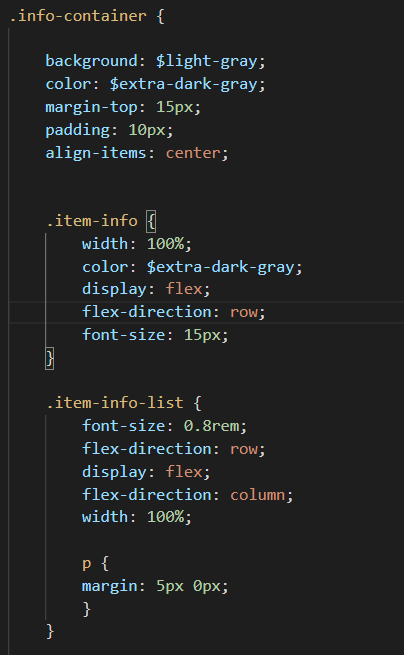
\includegraphics[width=75mm]{figures/Tekniske-valg/scssExample.PNG}
    \caption{Bruk av variabelnavn og nøsting av elementer i sass.}
\end{figure}
 
 \subsection{\textbf{Mobilutvikling}}
 For mobilutvikling snakker man ofte om native- og hybrid-utvikling, som er måter å utvikle applikasjonene på. Det å utvikle native gir deg ofte bedre ytelse i store applikasjoner, men gjør i gjengjeld at du må skrive flere separate kodebaser dersom du skal utvikle mot ulike operativsystem. Hybridutvikling er en måte å utvikle mot flere ulike plattformer. Fordelen med å kunne utvikle mot flere plattformer samtidig er at man ofte kan skrive én felles kodebase, men man ofrer gjerne en del av ytelsen som native-utvikling tilbyr deg, samt andre native-funksjoner dersom rammeverket ikke tilbyr dette. 
 
 

\subsection{\textbf{Angular}}
%Hvorfor Angular
Som nevnt tidligere ønsket vi å lett kunne lage eget design og egne uttrykk, og valgte derfor Ionic med Angular. Vår mobilapplikasjon skal være utformet som en en utvidelse av Millum Procurement, og ikke en frittstående applikasjon. Videre vil det å bruke samme rammeverk være hensiktsmessig ettersom Millum selv skal overta prosjektet. Det vil absolutt forenkle prosessene ved videreutvikling og drift for utviklingsteamet.

%Hva er Angular
Angular er et javascript-rammeverk og utviklingsplattform for å utvikle effektive og komplekse Single Page Applications (SPA) i HTML, CSS og TypeScript. TypeScript er et supersett av JavaScript som kompilerer til vanlig JavaScript. Single Page Applications betyr kort fortalt at man istedenfor å laste inn hele siden hver gang man navigerer, så laster man kun inn delene av siden som har forandret seg. Dette gjør at lastetiden er betydelig lavere enn i en tradisjonell webløsning. 

De fundamentale byggesteinen i Angular er NgModuler, komponenter og tjenestetilbydere. NgModuler er et kjernekonsept i Angular som er en del av enhver applikasjon og hjelper til med å samle viktige detaljer for kompilatoren og applikasjonens driftstid. De er spesielt nyttige for å organisere kode i funksjoner, lazy loading for routing, og lage gjenbrukbare biblioteker. NgModuler kan inneholde komponenter,  tjenestetilbydere og andre kodefiler.

Komponenter definerer hva som vises og inneholder logikk som definerer atferden. Ideelt sett er komponenten sitt ansvar kun selve brukeropplevelsen og ingenting mer. Komponentbasert programvareutvikling vektlegger separasjon av bekymringer med hensyn til den omfattende funksjonaliteten. Selve tankegangen er å skille ut deler av siden til egne komponenter som kan gjenbrukes. 

Tjenestetilbydere, heretter kalt ``Service`` er en bred kategori som omfatter enhver verdi, funksjon eller funksjon som en applikasjon trenger. En service er typisk en klasse med et smalt, veldefinert formål. Den skal gjøre noe spesifikt og gjøre det bra. Vår bruk av services blir utdypet i avsnittet \textbf{\ref{kommunikasjon}} 

% Hvordan brukte vi Angular
Vår bruk av Angular er ikke spesielt særegent fra andre Angular-prosjekter. Bruken av NgModuler er noe man må følge etter standard prosedyre, hvis ikke vil ikke applikasjonen kjøre. Derimot er det under bruk av komponenter og servicer man vil se forskjeller fra prosjekt til prosjekt. 


Tankegangen ved komponenter er å ta hvilken som helst nettside og dele opp i mindre deler. Eksempler på hva som typisk kan være et eget komponent er navigasjonsmenyen, en liste med nyhetsartikler og sidemenyer. Det vil selvsagt variere hvor mange tenkte komponenter man trekker ut etter man har drøftet omfang og kompleksitet for hele applikasjonen.




\subsection{\textbf{Ionic}}

%Hva er Ionic?

Ionic er et open source UI verktøy for å bygge effektive mobil- og web-appklikasjoner veb bruk av tidligere nevnte webteknologier HTML, CSS og JavaScript. Fokuset rammeverket har er på brukeropplevelsen og interaksjon. For hvert Ionic-prosjekt må man også spesifisere hvilket frontend-rammeverk man vil bruke. Ionic tilbyr bruk av Angular, Vue, React og Javascript. Dette samsvarer altså med valg av Angular som rammeverk.

Det Ionic tilbyr oss er ferdige UI komponenter som vi igjen kan velge å tilpasse etter vårt eget designutrykk. Bruken av Ionic sine komponenter er lett å ta i bruk. 

\begin{figure}[H] 
    \centering
    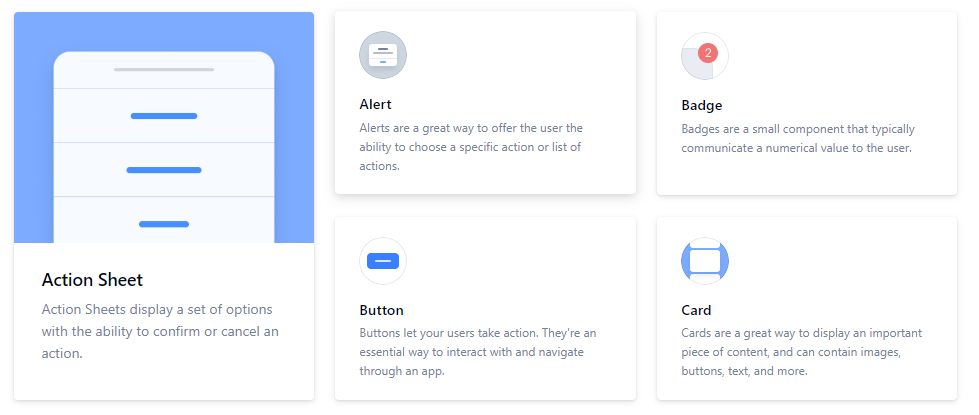
\includegraphics[width=\textwidth]{figures/Tekniske-valg/Ionic/Ionic-Components.PNG}
    \caption{Utsnitt av ferdige komponenter Ionic tilbyr}
\end{figure}

Et eksempel på å legge inn en knapp
\begin{lstlisting}
<ion-button>Ionic knapp!</ion-button>
\end{lstlisting}

\begin{figure}[H]
    \centering
    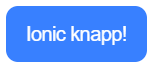
\includegraphics{figures/Tekniske-valg/ionicButtonExample.PNG}
    \caption{Standard <ion-button>.}
    \label{fig:my_label}
\end{figure}

%Hva er det i vår applikasjon som kommer fra Ionic rammeverket?
Siden Ionic har tilgang til operativsystemspesifikke funksjoner har man blant annet mulighet til å implementere søkefelt, knapper, dialoger og lister. Fordelen med å bruke disse er at de ofte er svært optimaliserte og kan lazy loades. Ulempen er at det kan være store variasjoner i design og uttrykk på tvers av plattformer, og man manuelt må overskrive disse dersom man ønsker like uttrykk på flere plattformer.

\begin{figure}[H] 
    \centering
    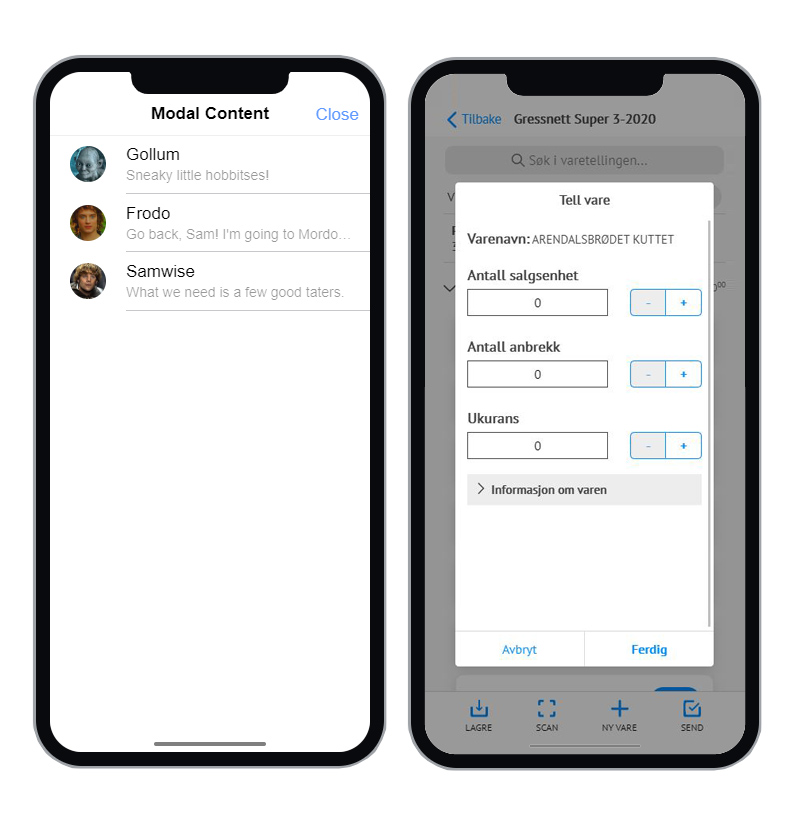
\includegraphics[width=\textwidth]{figures/Tekniske-valg/Ionic/modal.jpg}
    \caption{Ionic sin standard modal-komponent (t.v) sammenlignet med vårt designutrykk (t.h)}
    \label{modalComparison}
\end{figure}

I figuren ovenfor, \textbf{\ref{modalComparison}}, tar vi i bruk en modal, og så stilsatt den til å ikke ta hele skjermplassen. Dette for å vise brukeren at dette er en funksjonalitet knyttet til siden som vises i bakgrunnen, og at det ikke er en annen side de har navigert seg til. Et eksempel der vi bruker nativefunksjonalitet.

Ionic tilbyr også native API-løsninger. Disse gjør det slik at man kan ta i bruk funksjonalitet som kamerabruk, mobiltastatur eller fingeravtrykksleser. Ionic abstraherer og håndterer sikkerhetsutfordringer slik at vi kan få tilgang til for eksempel kameraet uten at vi må vite de spesifikke detaljene for hvordan iOS eller Android håndterer dette. 

Når det kommer til å lagring av informasjon på mobileneheten har Ionic flere muligheter og vi har valgt å ta i bruk Ionic Storage \cite{ionic:storage} for dette. Ionic Storage er en enkel lagringsmodul med ytterligere støtte for SQLite. Her kan vi altså lagre JSON objekter og nøkkel/verdipar til forskjellige lagringsmotorer, samlet gjennom ett grensesnitt.

\section{\textbf{Arkitektur}}
Softwarearkitektur refererer til de fundamentale strukturene og disiplinene til å lage et system. Å gjøre gode arkitekturvalg tidlig i prosessen gjør at vi får mulighet til å gjenbruke mest mulig kode og dele sentrale grensesnitt og funksjoner. I dette kapittelet skal vi drøfte arkitekturvalgene våre.

\subsection{\textbf{Kommunikasjon}} \label{kommunikasjon}
I enhver applikasjon er det viktig å definere hvordan kommunikasjonen skal foregå for å gjøre datafangst. Her går vi litt mer i dybden på hvordan kommunikasjonen foregår mellom mobilapplikasjonen og Millum sine API-er.

I løsningen vår er hver datastruktur eller tjeneste (varetelling, produkt osv.) delt inn i egne services. En service er ansvarlig for å tilgjengeliggjøre data når brukeren ber om det. Det kan være i form av at man ønsker å hente data relatert til en varetelling eller et produkt, eller at man ønsker å sende inn sin varetelling.

Servicen som er ansvarlig for å håndtere dette gjør et kall videre til en datatjeneste, heretter kalt “data service”. Data servicen er ansvarlig for selve kommunikasjonen mot API-ene. Kommunikasjonen foregår via Millum sin “Gateway” som igjen er ansvarlig for å lede kommunikasjonen til deres interne tjenester. Resultatet av handlingen data servicen ba om blir levert i en HTTP statuskode. Normalt sett hvis handlingen var vellykket får vi tilbake en statuskode ``200``. HTTP-protokollen er en godt utprøvd protokoll for kommunikasjon og blir brukt i de aller fleste webapplikasjoner. All kommunikasjon vi gjør over HTTP-protokollen blir gjort via JSON-format, som er en måte å strukturere dataobjekter på.

Avtalen med oppdragsgiver er at de leverer API-ene, og vi konsumerer disse igjen i applikasjonen. Dette er et bevisst valg med tanke på sikkerhet, men også med tanke på kompleksiteten og scopet til prosjektet vårt. 

\begin{figure}[H] 
    \centering
    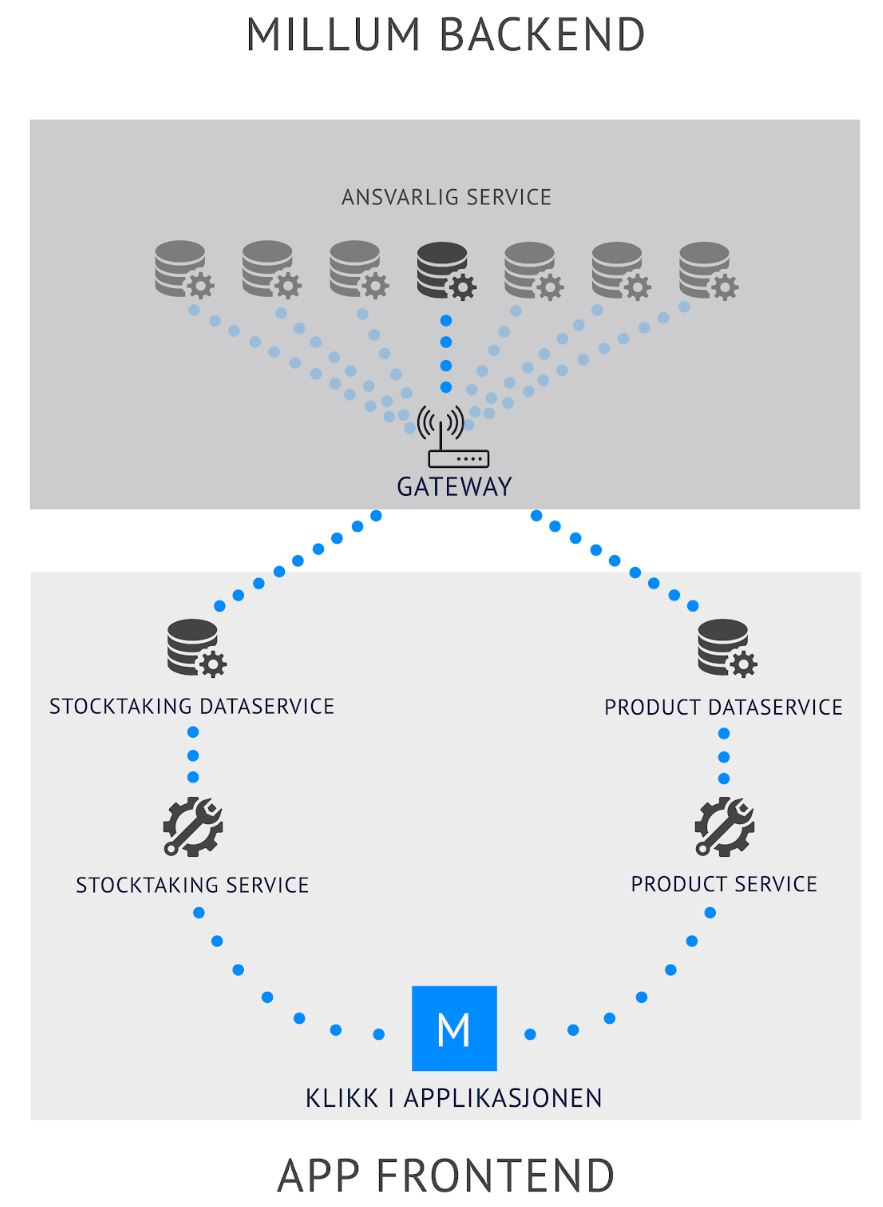
\includegraphics[width=\textwidth]{figures/Tekniske-valg/Arkitektur/kommunikasjon.JPG}
    \caption{Kommunikasjon mellom frontend og backend. Egen illustrasjon.}
\end{figure}

\subsection{\textbf{Utvikling}}
\subsubsection{\textbf{Versjonskontroll}}
For å ha kontroll på programvaren, endringshistorikk og ha mulighet til å utvikle parallelt benyttet vi oss av Git  og TFS (Team Foundation Server, senere Azure DevOps). Git er et distribuert versjonskontrollsystem og TFS fungerer som et komplett prosjektstyringsverktøy og vertstjeneste for kildekoden.

En av fordelene man har ved å bruke disse systemene er at man har mulighet til å lage avgreninger av kildekoden, heretter kalt \textit{branches}, slik at utviklerne kan jobbe isolert. Når utviklingsmålet er nådd i en branch kan utvikleren åpne en Pull Request, som er en forespørsel om å flette inn koden sin i en annen branch. Et typisk eksempel på dette er at man har gjort ferdig en user story og ønsker å flette inn denne i utviklingsbranchen slik at alle får tilgang på de siste endringene.

\begin{figure}[H] 
    \centering
    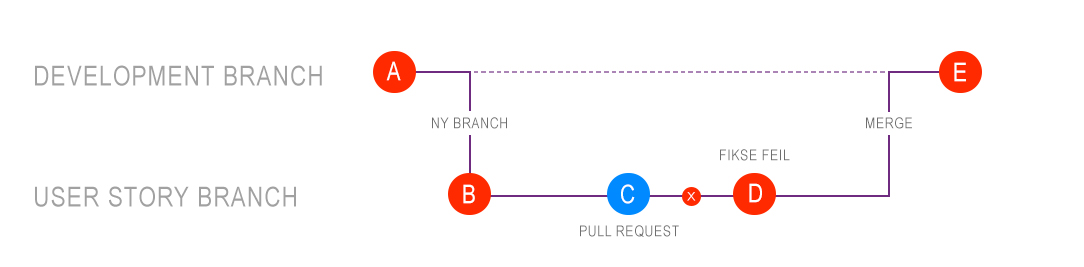
\includegraphics[width=\textwidth]{figures/Tekniske-valg/Utvikling/Git.jpg}
    \caption{Git branching og pull requests. Egen illustrasjon}
    \label{Git}
\end{figure}

Vi har laget egne regler for hvordan slik fletting skal gjennomføres. Det kan ikke være konflikter i koden på tidspunktet man ønsker å flette inn koden. Hvis det finnes konflikter må disse løses før flere handlinger kan gjøres. Når det ikke finnes konflikter i koden må en annen utvikler gå gjennom koden i det som typisk kalles et Code Review. Hensikten med et Code Review er å kvalitetssikre koden og utelukke åpenbare feil og mangler. Se \textbf{\ref{Git}} for hvordan våre regler fungerer. I mer komplekse applikasjoner har man ulike regler i ulike brancher slik at kun seniorutviklere, teamledere eller lignende har mulighet til å godkjenne Pull Requests til for eksempel Master Branch, som i de fleste tilfeller gjenspeiler produksjonskoden.

Som man ser i \textbf{\ref{Illustrasjon_versjonskontroll}} er det et klart strukturert hierarki. Master, Development og User Story branches definerer separate ansvarsområder i versjonskontrollsystemet. Måten vi har strukturert det på er slik :
\begin{itemize}
  \item \textbf{Master branch} - Gjenspeiler produksjonsmiljøet.
  \item \textbf{Development branch} - En stabil utgave av utviklingsmiljøet
  \item \textbf{User Story branch} - Egen branch for hver brukerhistorie.
  \begin{itemize}
      \item Klones lokal kopi av User Story branch på utviklerens maskin
      \item Disse må gjennom code review for å bli godkjent og merget inn i Development
  \end{itemize}
\end{itemize}

\begin{figure}[H] 
    \centering
    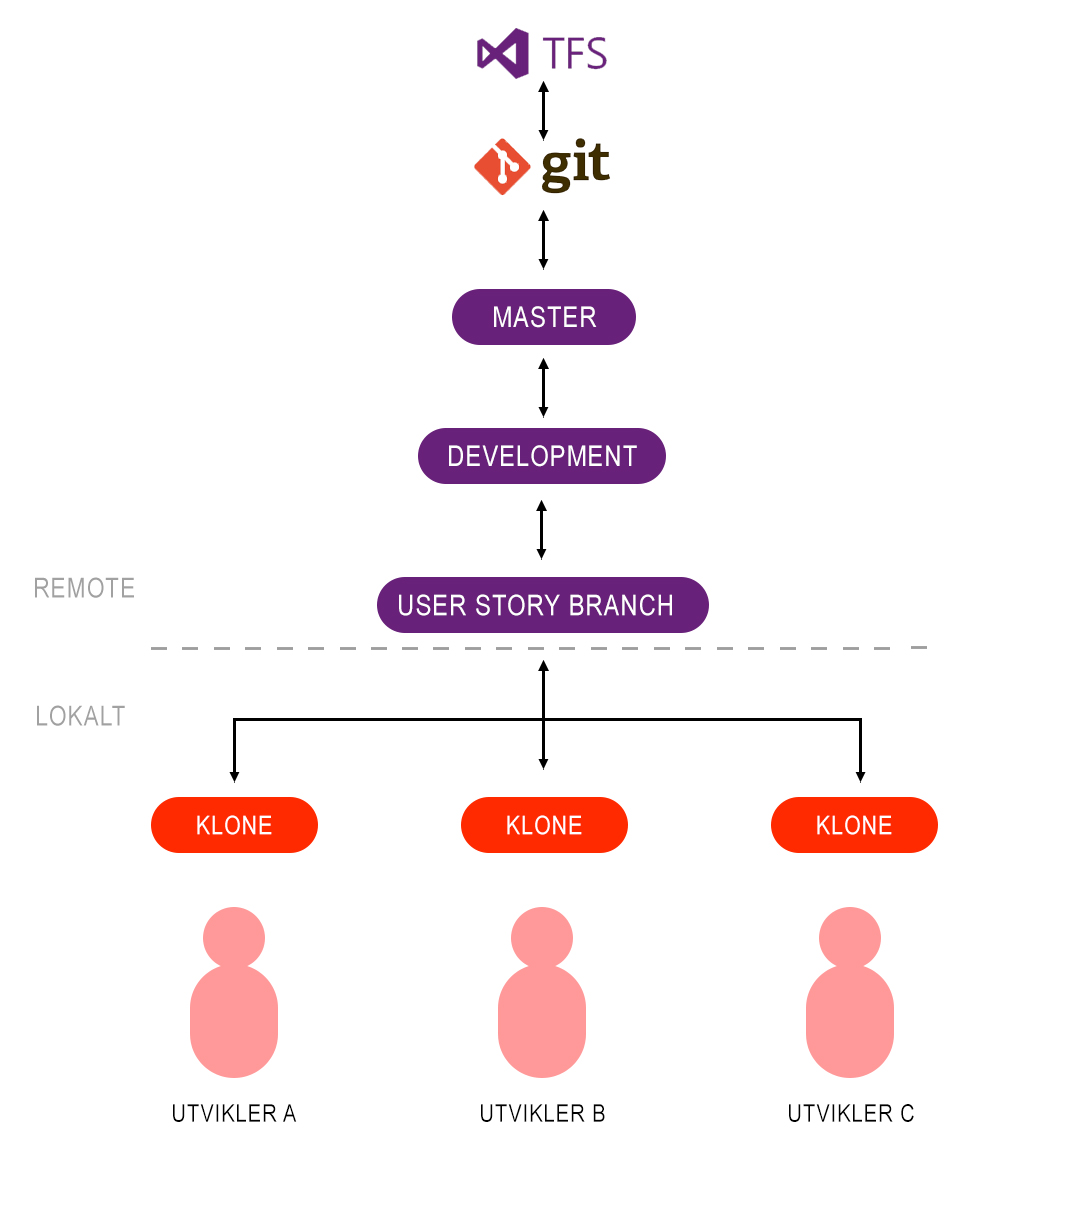
\includegraphics[width=\textwidth]{figures/Tekniske-valg/Utvikling/TFS.jpg}
    \caption{Illustrasjon av hvordan vi brukte et distribuert versjonskontrollsystem. Egen illustrasjon.}
    \label{Illustrasjon_versjonskontroll}
\end{figure}

\subsection{\textbf{Designmønster}}

I årevis har designmønsteret blitt brukt, men det har ikke alltid vært slik at man har vært bevisst på det. Det var arkitekten Christopher Alexander som i 1970-årene konkretiserte konseptet designmønstre innenfor arkitektur-konsepter \cite{christopheralexander}. Videre prøvde man å bruke disse konseptene innenfor programvare-utvikling. Det var derimot ikke før en av de mest kjente bøkene om designmønster,   
Design Patterns: Elements of Reusable Object-Oriented Software, kom på banen i 1994 at utviklere virkelig sperret opp øynene. 


\begin{table}[htbp]
  \centering
  \caption{De fire elementene som beskriver et designmønster \cite{gamma1995design} }
    \begin{tabular}{|l|l|}
\hline
Navnet        & \begin{tabular}[c]{@{}l@{}}Som sier oss noe om design-problemet,\\ løsningen og konsekvensene i ett til to ord\end{tabular} \\ \hline
Problemet     & \begin{tabular}[c]{@{}l@{}}Beskriver når man kan ta i bruk mønsteret\\  og i hvilken kontekst\end{tabular}                  \\ \hline
Løsnigen      & \begin{tabular}[c]{@{}l@{}}Beskrivere elementene som utgjør designet, \\ deres relasjoner, ansvar og samarbeid\end{tabular} \\ \hline
Konsekvensene & \begin{tabular}[c]{@{}l@{}}Beskriver resultatene og avveiningene\\  ved å bruke mønsteret.\end{tabular}                     \\ \hline
\end{tabular}
  \label{tab:addlabel}%
\end{table}%

Design Patterns-boken beskriver flere forskjellige mønstre, og videre går vi dypere inn i hva de forskjellige designmønstrene virker inn i applikasjons-strukturen.

\subsection{\textbf{Model View Controller}}
Model View Controller, MVC,  er et design pattern som deler inn programmet i tre sammenhengende elementer.

\begin{description}
  \item[$\bullet$ Model:] Beskriver programmets struktur uavhengig av grensesnittet. Modellen håndterer og bestemmer reglene og logikken til programmet.
  \item[$\bullet$ View:] Grensesnittet til programmet. Kan eksempelvis være en side eller et diagram.
  \item[$\bullet$ Controller:] Tar i mot hendelser fra viewet og interagerer med modellen.
\end{description}

To store fordeler med MVC er:

1. Du kan ha flere views knyttet til én modell for å gi forskjellige presentasjoner av samme data.

2. Endre viewet til å respondere på brukerinnspill uten å endre den visuelle representasjonen

 I vår løsning har vi hatt ansvar for å lage modellen og viewet, mens controlleren kommuniserer med oppdragsgivers egne tjenester. Et eksempel på hvordan dette henger sammen er at brukeren logger inn og skal hente sine varetellinger. Dette gjøres via et API-request til varetellingscontrolleren, som leverer tilbake informasjon som modellen strukturerer og videre presenterer i viewet. 

\subsection{\textbf{Rule of One og Single Responsibility}}
Single responsibility-prinsippet ble først introdusert av Robert C.Martin i hans artikkel med samme navn som en del av Principles of Object Oriented Design, gjort populært av hans bok Agile Software Development, Principles, Patterns, and Practices. Martin definerer responsibility i sin bok Agile Pratices, Patterns and Pratices in C\# som “In the context of the SRP, we define a responsibility to be a reason for change.” (Side 158). Definisjonen er noe tvetydig i formuleringen “a reason for change”. Martin fordyper denne definisjonen i et blogginnlegg kalt The Single Responsibility Principle.  

Rule of One bygger på et annet prinsipp kalt single responsibility. Kort beskrevet kan man si at alle komponenter, servicer og andre symboler kun skal gjøre én ting. Hensikten med dette er å gjøre filen lettere å lese, vedlikeholde og mer gjenbrukbar. I tillegg gjør det at koden er mer testbar, mindre utsatt for bugs og mindre avhengig av annen kode (også kjent som low coupling)

\subsection{\textbf{LIFT}}

\textit{"\textbf{Do} structure the app such that you can \textbf{L}ocate code quickly, \textbf{I}dentify the code at a glance, keep the \textbf{F}lattest structure you can, and \textbf{T}ry to be DRY"} 

Dette prinsippet skal hjelpe deg som utvikler å finne fram til kode raskt. Vi har valgt å følge LIFT-prinsippet på grunnlag av spørsmålet

\textit{Hvor raskt kan du åpne og jobbe i alle filene du trenger for å lage en funksjon? }

\textbf{Locate} gjør lokalisering av kode intuitivt og raskt. Det vil si å holde relaterte filer nær hverandre. For å jobbe effektivt ønsker man å kunne lokalisere filer raskt, spesielt når man ikke kjenner eller husker filnavnene. Å holde relaterte filer nær hverandre på et intuitivt sted sparer tid. En beskrivende mappestruktur gjør all verdens forskjell for deg og menneskene som kommer etter deg.

\textbf{Identify} betyr det å ha et beskrivende navn for filene slik at du umiddelbart vet hva filen inneholder og representerer. Her er det viktigere å være beskrivende med filnavnet og holde innholdet i filen kun relatert til navngivningen. Det vil si at man ønsker i aller sterkeste grad følger single responsibilty-prinsippet.

\begin{itemize}
    \item \textbf{Et eksempel på dårlig navngiving av en klasse:} public class X;
    \item \textbf{Et eksempel på god navngiving av en klasse:} public class StockTakingItem;
\end{itemize}


\textbf{Flat} omhandler selve mappestrukturen for prosjektet. Det å ha en flat mappestruktur betyr at man ønsker at en mappe skal maksimalt inneholde syv filer, og heller velge å lage undermapper om man overstiger antall filer. 
Eksempelvis har vi denne mappestrukturen i løsningen vår:

\begin{itemize}
    \item \textbf{Modul}
    \begin{itemize}
        \item \textbf{Smartkomponent 1} - Håndterer logikk
        \begin{itemize}
            \item \textbf{Dum komponent 1} - Håndterer f.eks et klikk og gir informasjon videre til smartkomponenten.
            \item \textbf{Dum komponent 2... osv}
        \end{itemize}
        \item \textbf{Smartkomponent 2... osv}
    \end{itemize}
    \item \textbf{Modul 2... osv}
\end{itemize}

\begin{figure}
    \centering
    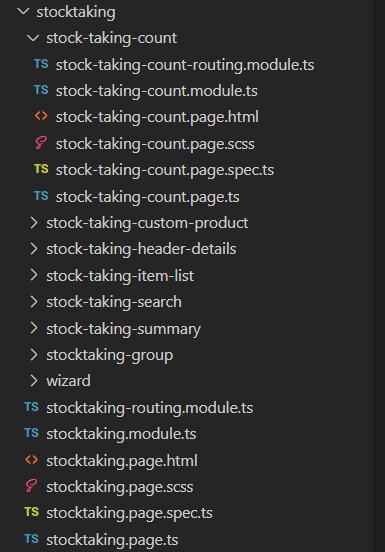
\includegraphics[width=75mm]{figures/Tekniske-valg/Utvikling/folderStructure.PNG}
    \caption{Utsnitt av mappestruktur i prosjektet.}
    \label{mappestruktur}
\end{figure}


På en annen side mener psykologer at mennesker begynner å slite når antallet nærliggende interessante ting overstiger ni \cite{miller1956magical}. 
Så når en mappe har ti eller flere filer, kan det være på tide å lage undermapper. Baser avgjørelsen din på ditt komfortnivå. Bruk en flatere struktur til det er en åpenbar verdi å lage en ny mappe

\textbf{Try to be Dry}, altså ikke repeter deg selv. For eksempel gir det ikke noe mening å lage en fil hetende "stock-taking-list-\textbf{view}.component.html". Dette er en HTML-fil og HTML-filer beskriver jo kun det som vises. Det vil dermed bli repetisjon at filnavnet skal inneholdet ordet ``\textbf{view}``.

\chapter{\color{Millum}\textbf{Design og utforming}}
I dette kapittelet gjør vi rede for vår prosess tilknyttet utforming og noen av de konkrete designvalgene vi har gjort for å hjelpe brukeren i løsningen.

\section{\textbf{Fremgangsmåte}}
Ved å bruke en fremgangsmåte kalt \textit{Minimum Viable Product} har vi hatt muligheten til å lage et grunnskall for applikasjonen hvor mye av kjernefunksjonaliteten er på plass før vi definerer uttrykket. Ved å bruke denne fremgangsmåten har vi hatt mer tid til å konseptualisere og skissere uttrykkene i applikasjonen

\section{\textbf{Farger}}
Siden mobilapplikasjonen er en utvidelse av Millum Procurement og oppdragsgivers produktportefølje har vi valgt å følge deler av deres fargepalett (\textbf{\ref{fig:farger}}) samt operativsystemene sine egne farger for søkefelter og lignende. Primærfargen kalles for \textbf{Millum Blue} og er en kraftig blåfarge som skal brukes der man ønsker brukerens oppmerksomhet, for eksempel viktige knapper som ``tell`` eller ``lagre``. Sekundærfargen kalles \textbf{Extra Dark Gray}, som er en mørk gråfarge skal brukes på alle tekster hvor fargekontrastene tillater det. 

\begin{figure}[H] 
    \centering
    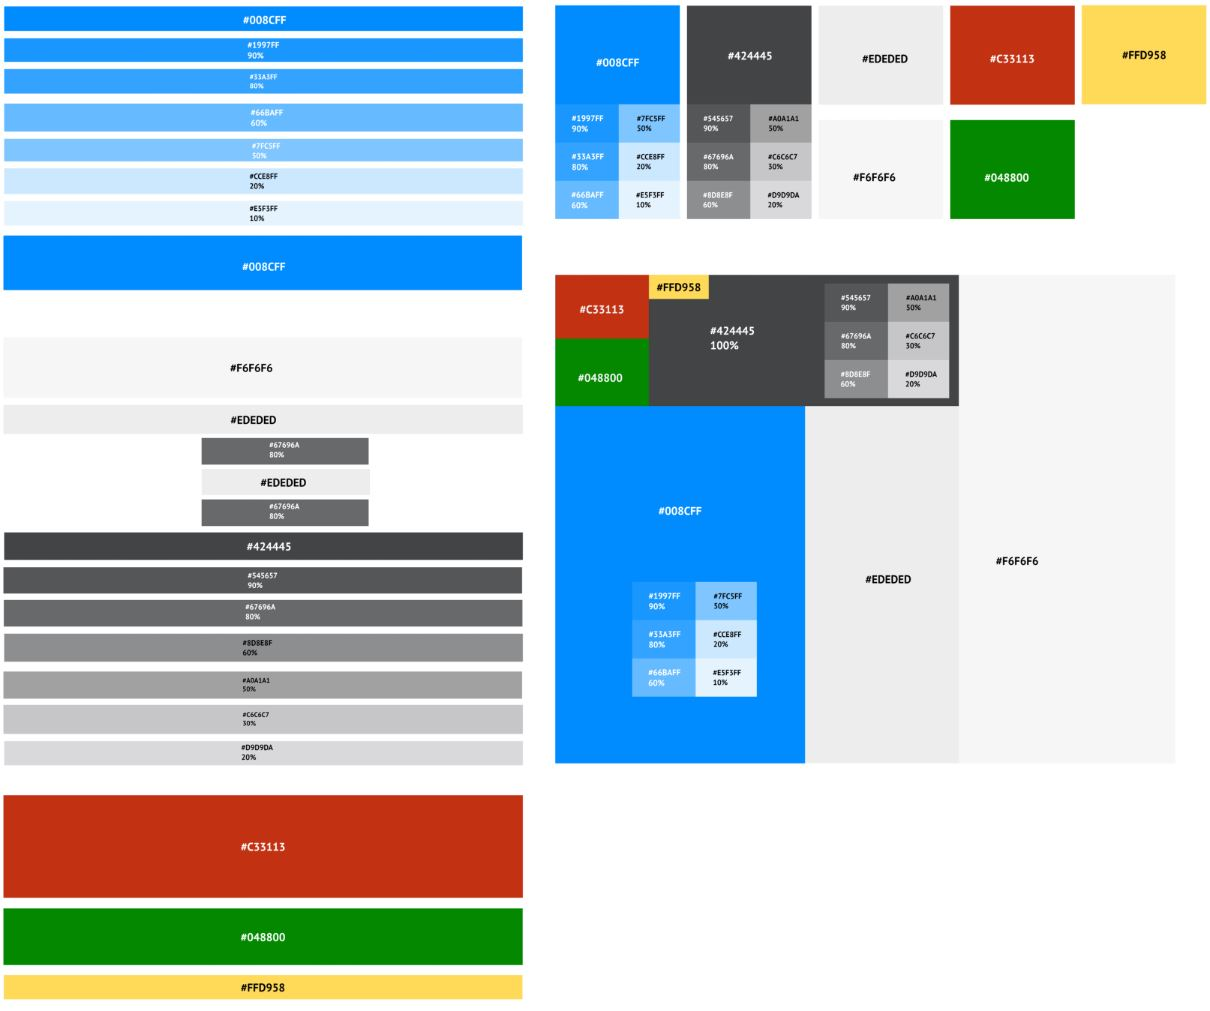
\includegraphics[width=100mm]{figures/Design-utforming/Fargepalett.JPG}
    \caption{Den komplette fargepaletten til Millum.}
    \label{fig:farger}
\end{figure}

\section{\textbf{Skisser og prototyper}} \label{Skisser}
I dette avsnittet går vi mer i dybden på skissene og prototypene vi lagde og hvordan disse utviklet seg til den endelig løsningen. \textit{Å lage skisser bidrar til å foreslå, utforske og formidle idéer (Rojas 2019).}

\section{\textbf{Designets evolusjon}}
Ved å jobbe i sprintsykluser hadde vi muligheten til å se evolusjonen av designuttrykket vårt underveis i hele prosessen. Som nevnt i \textbf{\ref{Skisser}} lagde vi lavnivå-skisser som viste ønsket funksjonalitet, men ikke pikselperfekte detaljer. Grunnen til at vi laget lavnivå-skisser er at vi hadde et ønske om å inkludere oppdragsgiver i prosessen ved å kontinuerlig få tilbakemeldinger på design og oppførsel.

I tredje sprint hadde vi mye av funksjonaliteten på plass og bestemte oss for å jobbe med en del av tilbakemeldingene vi hadde fått på sprintpresentasjonene. I eksempelet (\textbf{\ref{fig:evolusjon_dashboard}}) ser man hvordan designuttrykket har endret seg på tre sprintsykluser. 

\begin{figure}[H] 
    \centering
    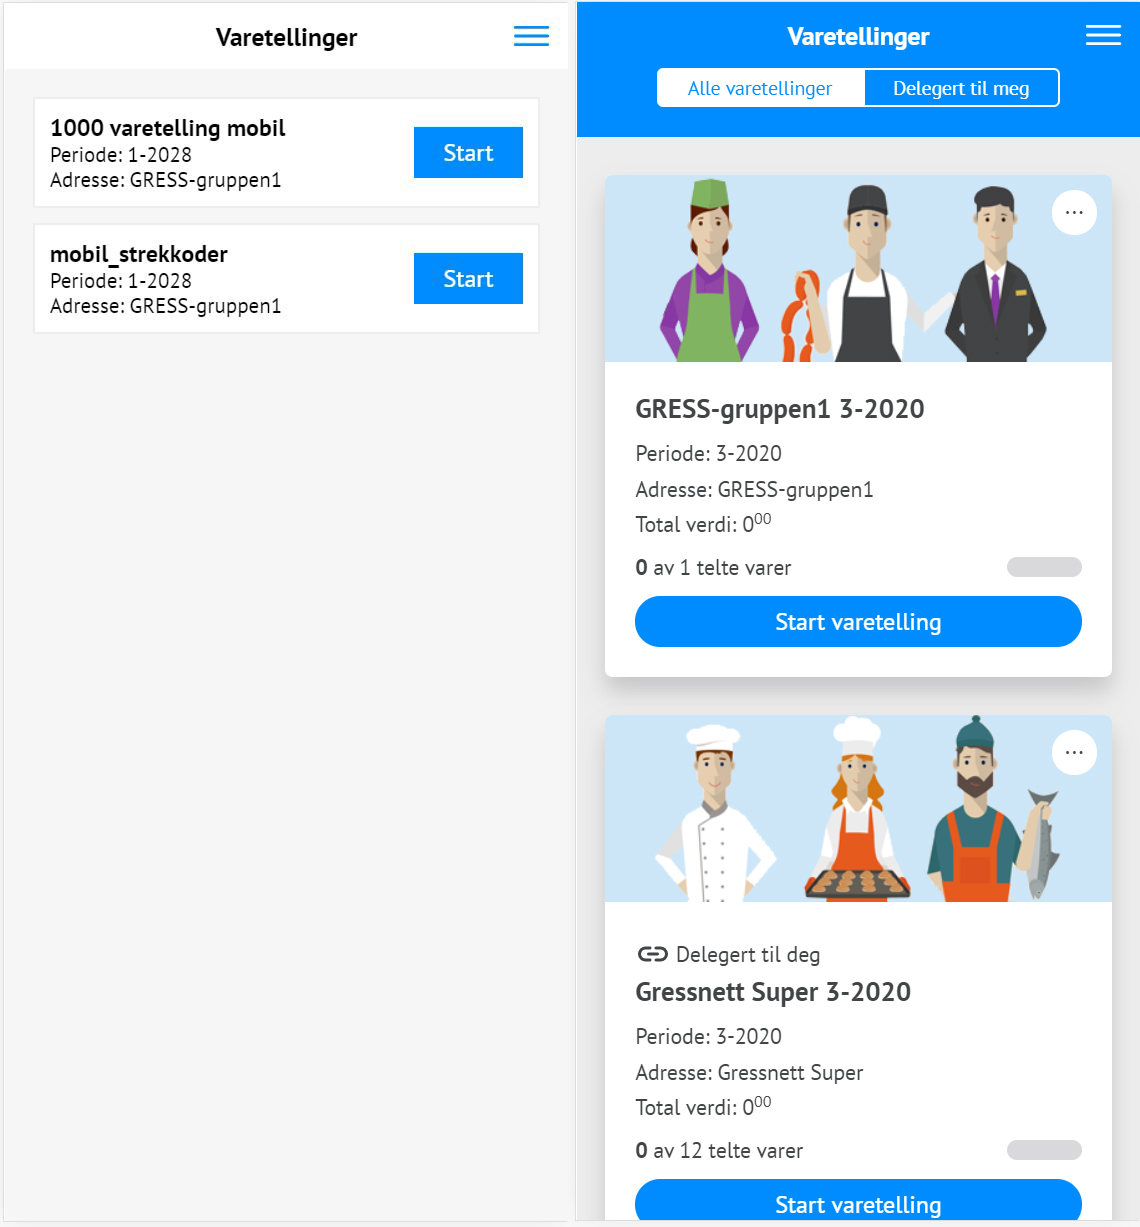
\includegraphics[width=100mm]{figures/Design-utforming/Evolusjon_dashboard.jpg}
    \caption{Dashboard i sprint 3 (t.v). Dashboard i sprint 6 (t.h).}
    \label{fig:evolusjon_dashboard}
\end{figure}

\section{\textbf{Design for flere flater}}
I samsvar med spørreundersøkelsen vi gjennomførte (\textbf{REF SPØRREUNDERSØKELSE}) så vi behovet for å utvikle løsningen for både mobil og nettbrett. Den åpenbare grunnen til å designe for flere flater er at vi støtter enhetene til flere i målgruppen, samt at vi kan utnytte plass bedre på større enheter. Eksempelvis ved å vise label og inputfelt ved siden av hverandre på nettbrett, men over/under på mobil som vist i figur \textbf{\ref{fig:tablet_vs_mobil}}. Vi skriver mer om universell utforming i neste avsnitt.

\begin{figure}[H] 
    \centering
    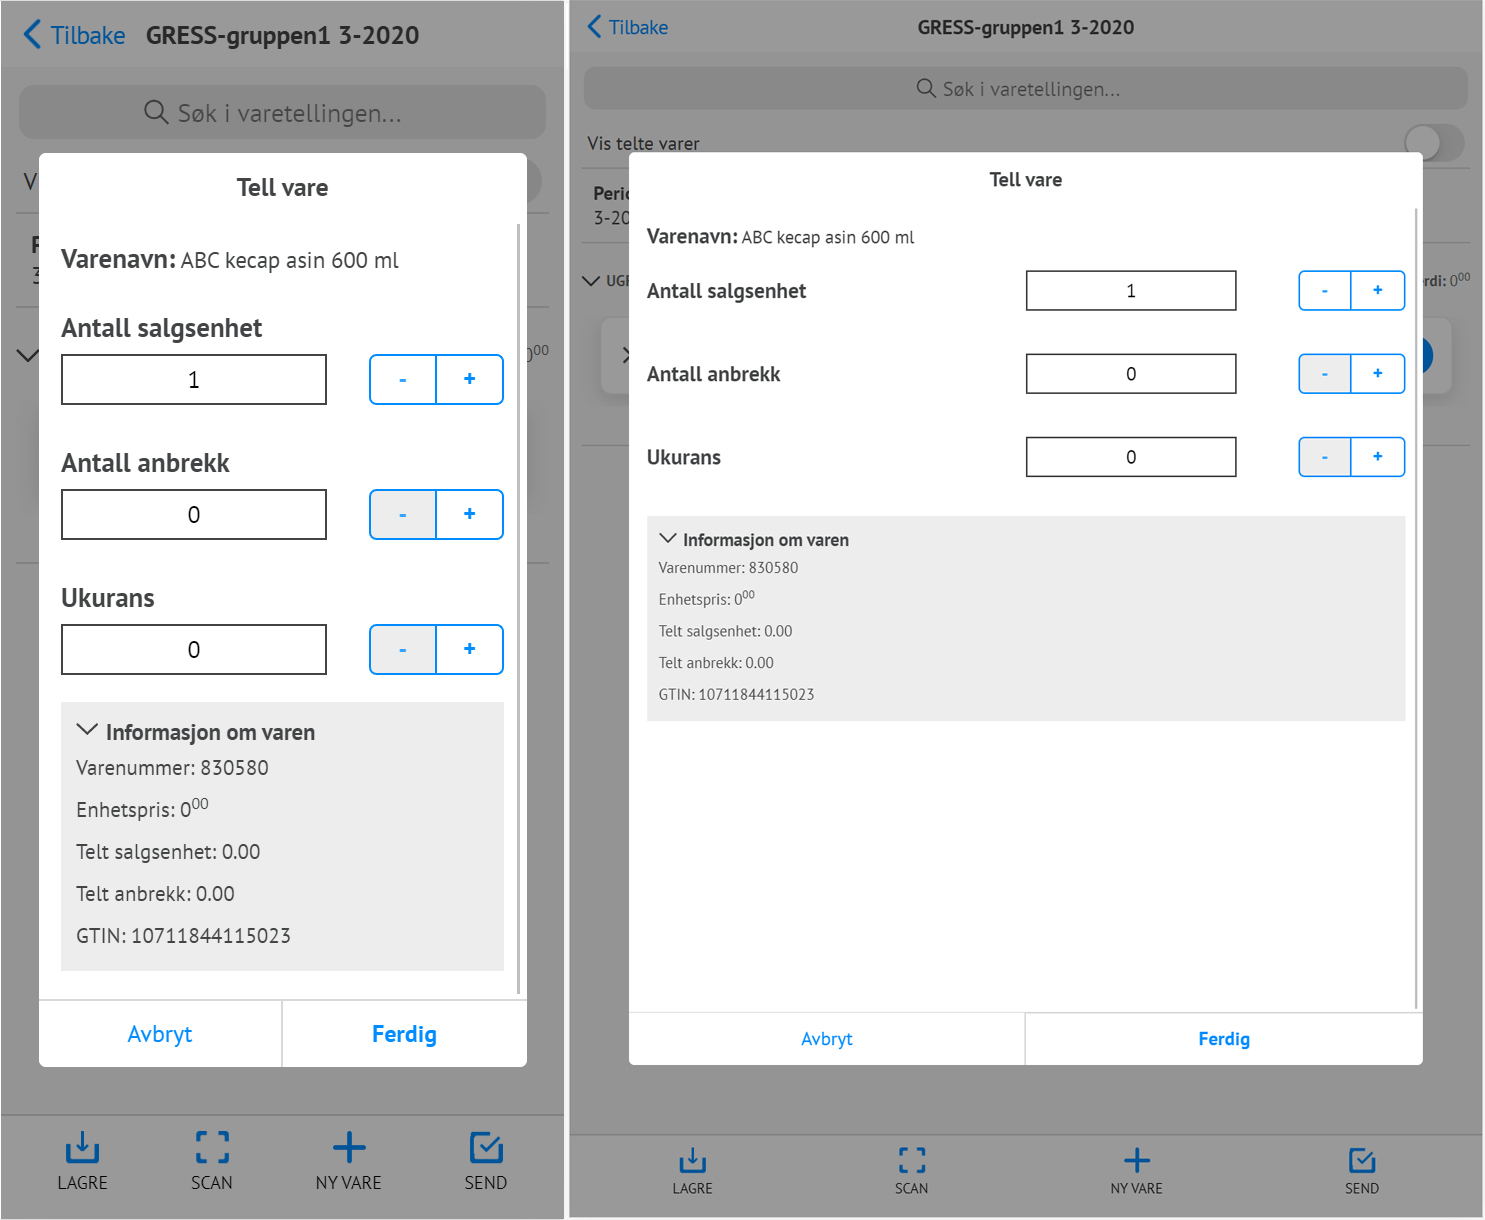
\includegraphics[width=100mm]{figures/Design-utforming/Tablet_vs_mobil.jpg}
    \caption{Mobilvisning av tellemodus (t.v). Nettbrettvisning av tellemodus (t.h).}
    \label{fig:tablet_vs_mobil}
\end{figure}

\section{\textbf{Universell utforming}} \label{Universell_utforming}
Universell utforming handler om å utforme omgivelsene slik at vi tar hensyn til variasjonen i funksjonsevne hos innbyggerne, inkludert personer med nedsatt funksjonsevne.\cite{digiuniversell} Hensikten er å kunne nå alle målgruppene gjennom en og samme løsning. Forskriften om universell utforming av IKT-løsninger stiller krav om at nettsider må oppfylle 35 av 61 suksesskriterier i “Retningslinjer for tilgjengelig webinnhold" \cite{digiwcag}. Mobilapplikasjonen vi har utviklet er omfattet da den må laste ned informasjon fra internett for å fungere.

Universell utforming er mer enn bare å tilrettelegge for mennesker med funksjonsnedsetting, men også eksempelvis mennesker med annet morsmål, lav domenekunnskap, vanskeligheter for å bruke mobiltelefon og så videre. Det har vært viktig for oss å ikke bare tenke på universell utforming, men aktivt inkludere det underveis i prosessen. Vi vet at mange av kundene til Millum har andre morsmål enn norsk og har derfor vært opptatt av å inkludere flere språk, selv om dette ikke var et formelt krav fra oppdragsgiver.

Det kan være vanskelig å følge alle retningslinjene, men det er lettere gjort når man inkluderer det i hele prosessen. Mange av våre designvalg har vært i tråd med artikler og forskning gjort av Nielsen Norman Group, som ansees for å være en av verdens fremste på forskningsbasert universell utforming og brukeropplevelse. Eksempelvis kan vi vise til det som kalles for \textit{input steppers}. Det vil si et inputfelt med tilhørende knapper for pluss og minus. 
\begin{figure}[H] 
    \centering
    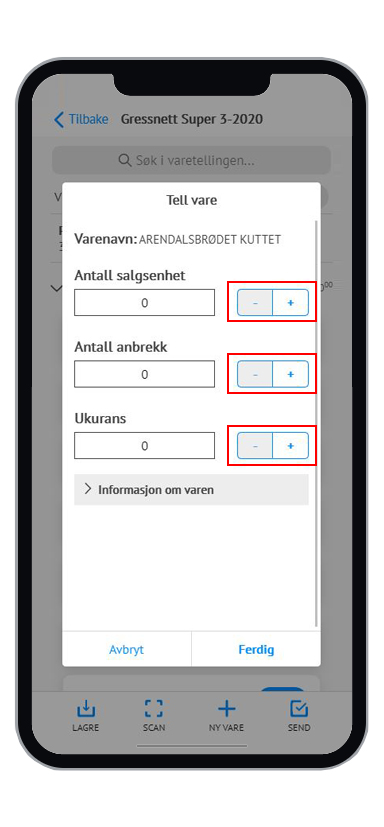
\includegraphics[width=75mm]{figures/Design-utforming/universell-utforming.jpg}
    \caption{Inputfelt (t.v). Input stepper markert i rød boks (t.h).}
    \label{fig:DesignInputStepper}
\end{figure}

En av de sentrale funksjonalitetene i løsningen er å kunne telle antallet man har av en vare. Vi var derfor helt avhengig av en god brukeropplevelse og har gjennom flere iterasjoner og bruk av forskning fra Nielsen Norman Group\cite{nngsteppers} kommet frem til en god måte å telle på. Ved å kunne taste inn store tall på eksempelvis vekt og volum, men samtidig kunne trykke en eller to ganger på en vare det ikke finnes mange av gir vi brukeren to valg og forenkler prosessen (\textbf{\ref{fig:DesignInputStepper}}). Universell utforming handler også om brukervennligheten, som vi kommer tilbake til i neste avsnitt om designprinsipper.

\section{\textbf{Designprinsipper}}
\subsection{\textbf{Bekreftelsesprinsippet}}
\textit{Bekreftelsesprinsippet er en teknikk brukt til kritiske handlinger, input eller kommandoer.}  (Lidwell 2003, s. 44)

Bekreftelse er en to-stegs operasjon som krever en handling fra brukeren i forkant av visning av dialogen. For å unngå at brukeren gjennomfører handlinger med katastrofale konsekvenser, som å gå ut av varetellingen uten å lagre bruker vi bekreftelsesdialoger for å hjelpe brukeren med å forstå konsekvensen av handlingen og gir de et valg om å likevel gjennomføre handlingen (som vist i \textbf{\ref{Bekreftelsesdialog}}).

\begin{figure}[H] 
    \centering
    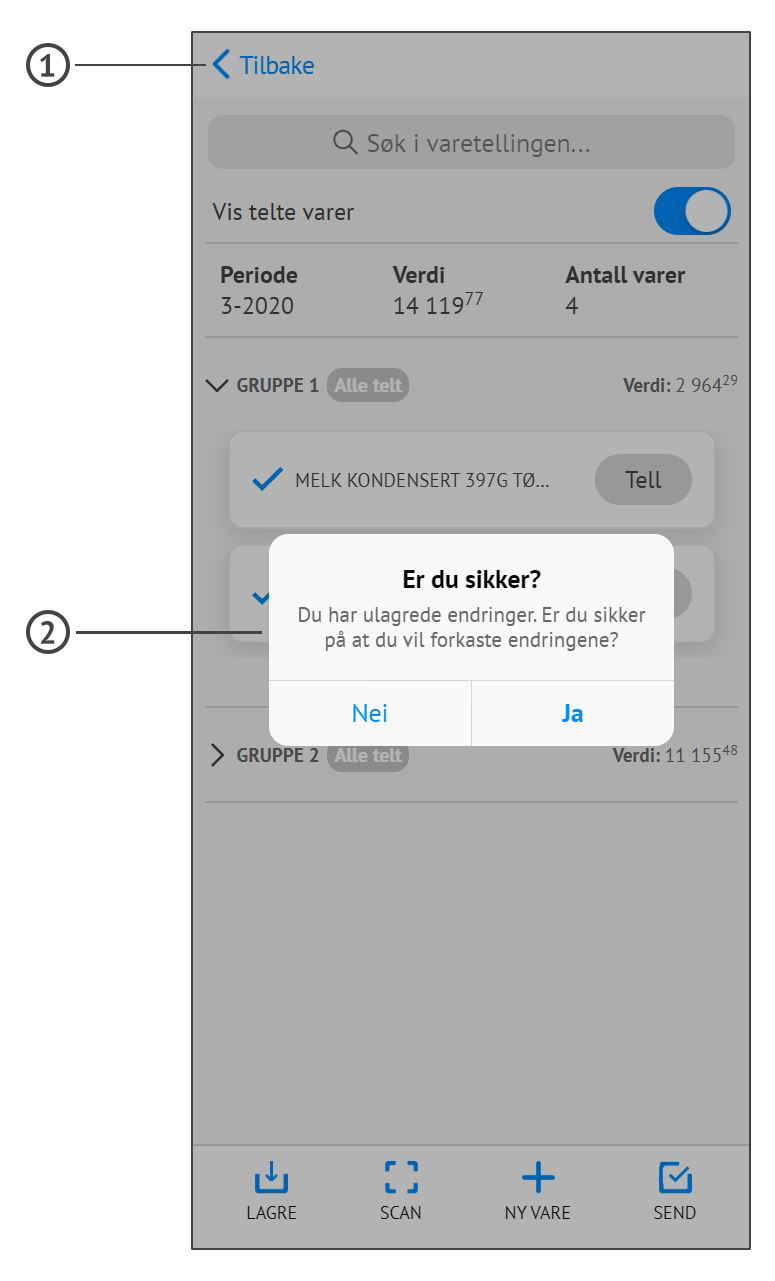
\includegraphics[width=75mm]{figures/Design-utforming/principle_confirmation.JPG}
    \caption{Bekreftelsesdialog (2) etter å ha trykket på tilbakeknapp (1) mens det foreligger ulagrede endringer}
    \label{Bekreftelsesdialog}
\end{figure}

\subsection{\textbf{Konsekvent design}}
William Lidwell skriver at brukervennligheten til et system forbedres når lignende deler uttrykkes på like måter. (Lidwell 2003, s. 46)

Ved å være konsekvent i design, tilbakemeldinger til brukeren, fargevalg, font o.l. Her økes ikke bare brukervennligheten i mobilapplikasjonen, men bygger også på helheten i produktporteføljen ettersom brukeren allerede kjenner til grensesnittet i handelsportalen Millum Procurement som vist i (\textbf{\ref{Konsekventdesign}}). 

\begin{figure}[H] 
    \centering
    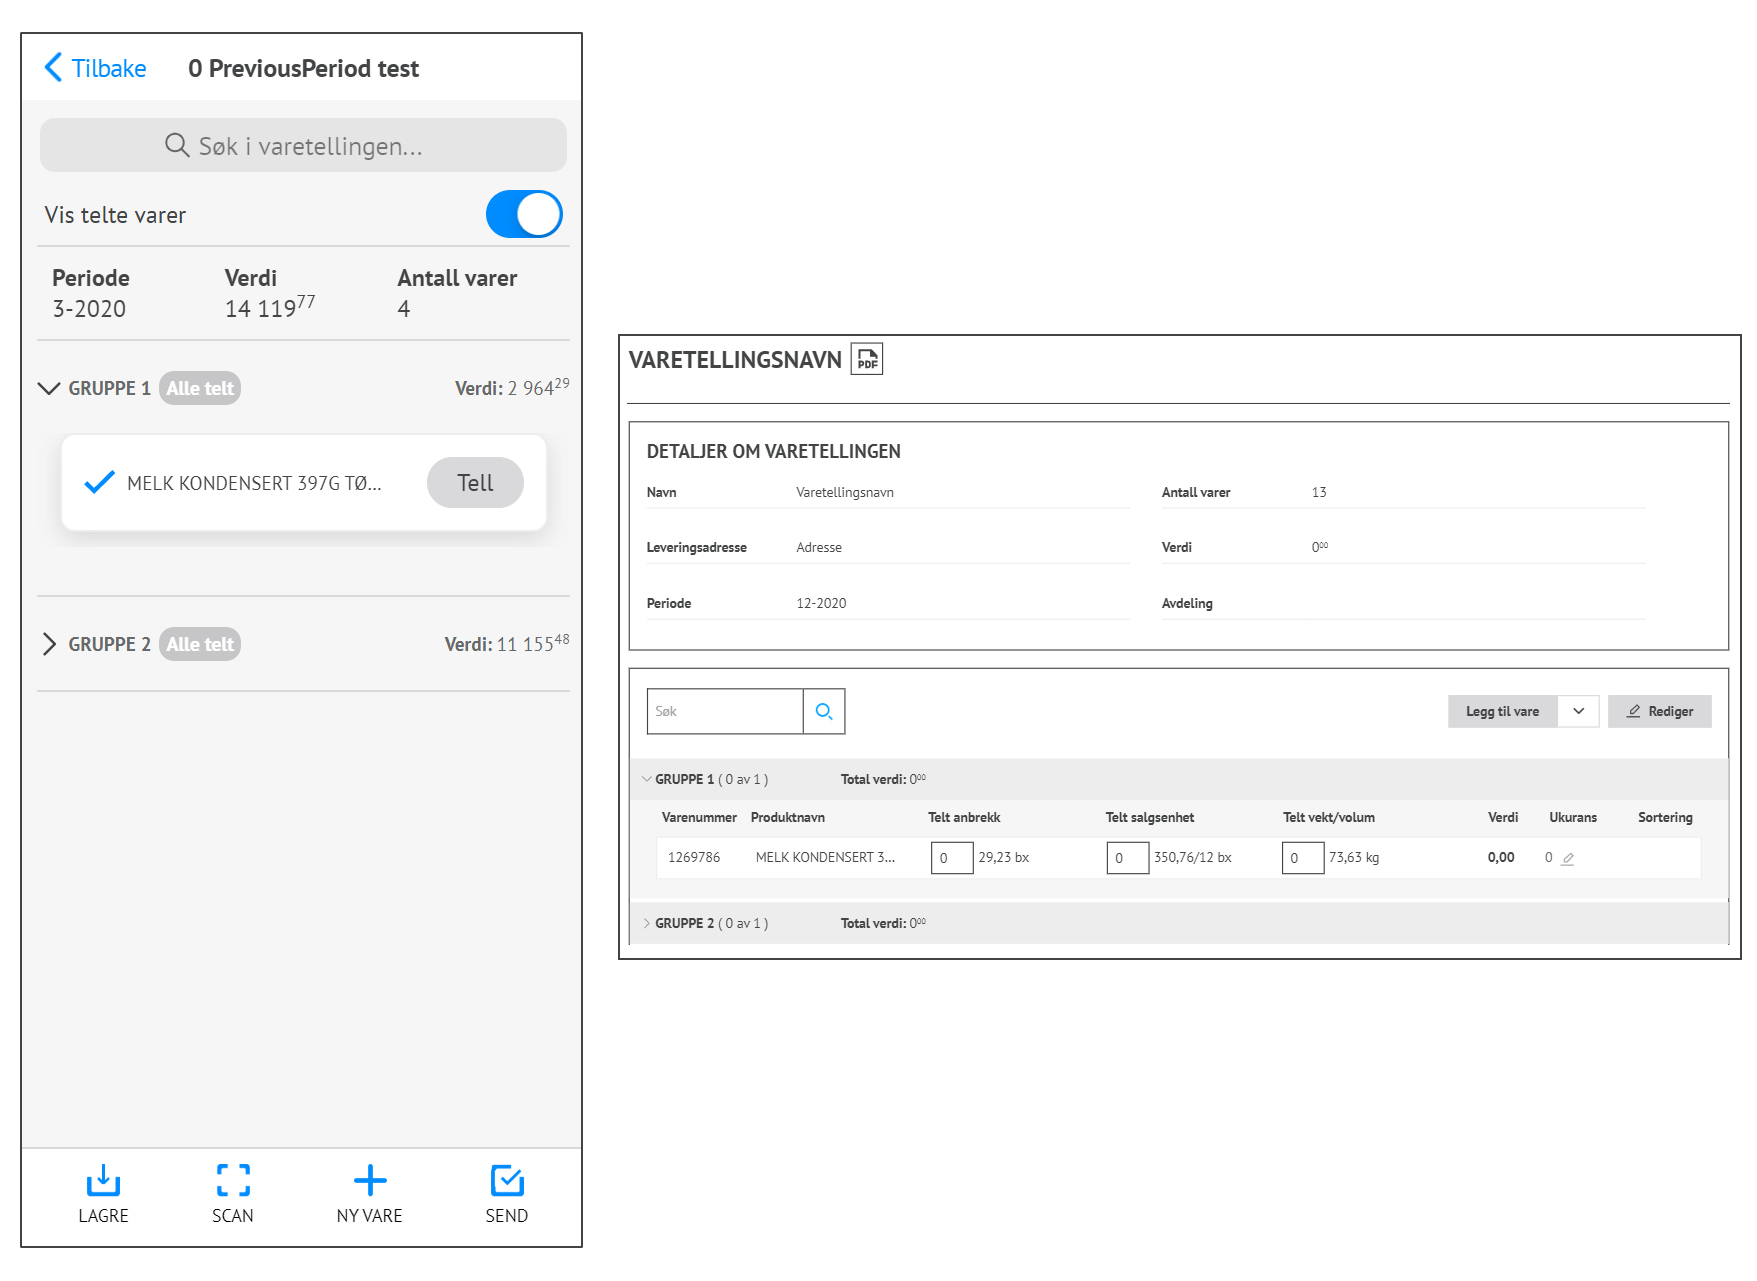
\includegraphics[width=150mm]{figures/Design-utforming/principle_consistency.jpg}
    \caption{Designuttrykk i mobilapplikasjonen (t.v) mot designuttrykket i webløsningen (t.h)}
    \label{Konsekventdesign}
\end{figure}

%%Avsnitt om flyt i applikasjonen med tanke på at vi konsekvent har valgt "3 sideer" slik at bruker kan effektivt navigere seg raskt igjennom arbeidet med å gjennomføre en varetelling
\subsection{\textbf{Proximity}}
\textit{Elements that are close together are perceived to be more related than elements that are farthel- apart.}(Lidwell 2003, s. 160).

Dette er et viktig prinsipp, siden feilvalg kan føre til frustrasjon for brukeren. Å gruppere elementer som hører sammen gjør det lettere for brukeren å forstå sammenhengen. Dette fører også tilbake til forrige punkt om konsekvent design. Dette ser vi flere ganger gjennom applikasjonen, eksempelvis i tellemodusen hvor et inntastingsfelt har tilhørende pluss- og minusknapper, eller i bunnmenyen hvor knappene har tilhørende tekst.

\subsection{\textbf{Chunking}}
Chunking er et prinsipp hvor formålet er å øke hukommelsen til brukeren i løsningen. Ofte blir en bruker overveldet av all informasjon man har tilgjengelig og prinsippet sier derfor at man bør bryte opp informasjon i mindre deler og konkretisere innholdet. Man må være sikker på at innholdet man lager er nødvendig og enkelt nok til å forstå slik at brukeren ikke bare oppfatter budskapet, men husker formålet med innholdet. Eksempler på hvordan vi har benyttet oss av dette prinsippet i løsningen vår er så enkle grep som å lukke seksjoner med informasjon som ikke er helt nødvendig å presentere for brukeren til enhver tid, som vist i figur \textbf{\ref{Informasjon_lukket}}

\begin{figure}[H] 
    \centering
    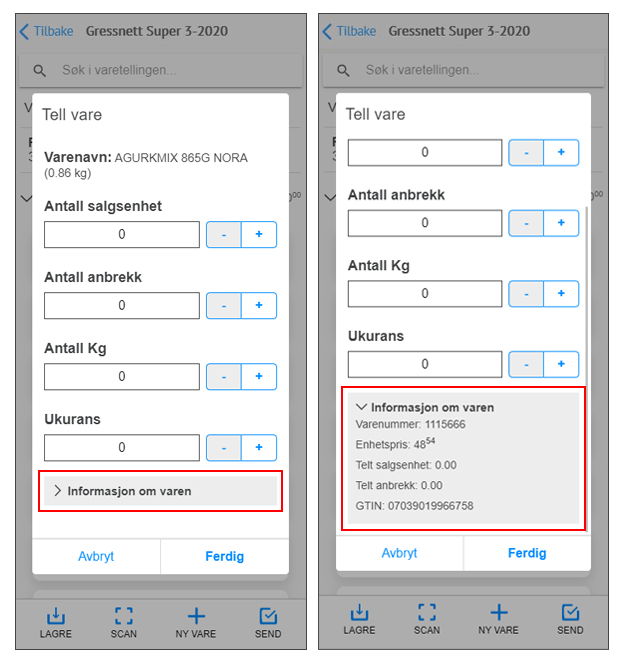
\includegraphics[width=100mm]{figures/Design-utforming/information_collapsed.jpg}
    \caption{Informasjon om varen lukket (t.v). Informasjon utvidet (t.h)}
    \label{Informasjon_lukket}
\end{figure}

\subsection{\textbf{Mapping}}
I denne konteksten betyr \textit{mapping} relasjonen mellom funksjonalitet og utseende. Trykker du på lysbryteren på veggen forventer du at lyset skrus av eller på, og ikke at du skrur på radioen. Dette gjelder også i design av produkter, og vi har vært bevisste på dette.

%Trykker du på en knapp forventer du kanskje en hvis form for funksjonalitet fra trykket i forhold til hvilket ikon eller tekst knappen er utsmykket med. For eksempel kan det tenkes at en knapp med et profil ikon åpner en profil side, med informasjon som: brukernavn, passord, gatenavn, innstillinger osv. Vi har brukt logisk Mapping ved å gi knapper ikoner og tekster (noe om logisk ikon bruk..). Et eksempel på dette... (sett in screen)

\section{\textbf{Brukervennlighet}}
 
 Brukervennlighet, eller \textit{Usability} på engelsk handler om hvor enkel løsningen er å forstå og å bruke. Man kan argumentere for at brukervennligheten er summen av de prinsippene vi har fulgt, ved å gjøre konkrete og gjennomtenkte designvalg gjennom hele prosjektet. I den moderne verden har brukervennlighet blitt viktigere enn noen gang, og om brukeren ikke forstår eller misliker innholdet så vil ofte brukeren slutte å bruke løsningen. Vi ønsker at brukeren skal oppleve verktøyet som intuitivt, og at arbeidsprosessen forbedres ved bruk av løsningen.
     
     %I den moderne verden har brukervennlighet blitt mer viktig enn noen gang. Om bruker ikke forstår eller misliker funksjonalitet til en applikasjon er det lett at bruker ikke vil fortsette å bruke applikasjonen. Vi leser ikke lenger manualer eller håndbøker ved bruk av applikasjoner.  I en studie medgir Google at hele 53\% av brukere forlater mobilapplikasjonen om siden tar over 3 sekunder å lastes inn(). I forhold til vår applikasjon er dette mindre relevant ettersom vår applikasjon er et arbeidsverktøy. Det viktigste er at arbeids prosessen utføres raskt og effektivt. Det er så klart også viktig at bruker liker arbeids verktøyet, spesielt ettersom vår applikasjon er et alternative, ikke en nødvendighet. %
     
     \textit{For intranets, usability is a matter of employee productivity. Time users waste being lost on your intranet or pondering difficult instructions is money you waste by paying them to be at work without getting work done.}(Jakob Nilsen, 3 Januar. 2012, NNGroup)
     
     
     
     
    
 

\chapter{\textbf{Bruker og marked}}
\section{\textbf{Brukerundersøkelse}}
Det ble i andre sprintsyklus av prosjektet utarbeidet og sendt ut en spørreundersøkelse til administratorer hos Millums kunder. Formålet med undersøkelsen var å kartlegge hva slags enheter organisasjonene innehar, hva slags og hvilken versjon av operativsystem som brukes, hvor mange som deler på hver enkelt enhet og hvordan de ansatte gjennomfører varetellinger.

\subsection{\textbf{Forberedelser}}
Vi hadde en del antagelser i forkant av undersøkelsen som dannet grunnlaget for hva vi ønsket å spørre om. Det ville for eksempel være interessant å vite om hvor mange som deler én enhet med tanke på innloggingsystemet vårt. Det kunne være forvirrende for bruker om de alltid skulle måtte logge ut av enheten når de tar den i bruk. Bruk av operativsystem og versjon var av betydning for oss fordi vi måtte tilrettelegge for dette siden enkelte kritiske funksjonaliteter ikke er tilgjengelig på eldre enheter samt at applikasjonen kan skalere forskjellig på ulike enheter. Vi ville også vite hvor ofte og hvordan bedriften utfører en varetelling. Denne innsikten er viktig i forbindelse med flyt i applikasjonen. Avslutsningsvis fant vi ut at det kunne være fint for deltager å kunne legge inn egne kommentarer til oss dersom det var annen informasjon de mente var relevant for oss.

For å kartlegge tidsbruk og avdekke feil/mangler ba vi ansatte internt i Millum ta undersøkelsen, noe som resulterte i flere konkretiseringer og endringer i undersøkelsen.

\subsection{\textbf{Gjennomføring}}
I forkant av spørreundersøkelsen tok vi kontakt med markedsavdelingen til Millum for å få en liste over kontaktpersoner som var interessante å sende undersøkelsen til. Dette resultere i en liste over de 22 administratorene vi leverte undersøkelsen til. Mange av kundene ønsker å bidra til utvikling av arbeidsverktøyene deres og vi valgte derfor å sende ut én e-post til hver organisasjon med informasjon om undersøkelsen, tidsbruk og hva undersøkelsen innebar.

\subsection{\textbf{Resultat}}
Vi lot undersøkelsen stå åpen i to uker så organisasjonene hadde mulighet til å videresende undersøkelsen internt til de ulike brukerstedene. Vi fikk derfor 64 svar fra de 22 organisasjonene vi kontaktet.

De viktigste innsiktene vi fikk i denne fasen gikk på andelen iOS/Apple-brukere og Android-brukere og hvordan de i dag gjennomfører varetellinger. Mange av tilbakemeldingene vi fikk dreide seg om muligheten til å kunne lese av strekkoden på varene på lageret og telle disse. Vi kunne derfor vite at vi traff bra med de tekniske valgene vi har gjort, siden vi utviklet samtlige ønsker som ble spilt inn. 


\section{\textbf{Konkurrenter}}
Det finnes flere direkte konkurrenter til en varetellingsapplikasjon, men siden applikasjonen er integrert i en handelsløsning som Millums eksisterende kunder bruker kan man anta at de færreste av disse er direkte konkurranse for Millum. 

Grossisten ASKO leverer ikke bare mat i kongeriket, men også handelsportaler og en varetellingsapplikasjon knyttet til denne. Applikasjonen deres tilbyr mye av den samme funksjonaliteten, men mangler et brukerrettet design og helhet som vi tilbyr i løsningen vår. En av funksjonalitetene som er sterkt etterspurt av Millum sine kunder er muligheten til å håndtere avvik i varetellingen. Det vil si varer som enten ikke er lagt inn i varetellingen på forhånd, varer man ikke får treff på via strekkode eller lignende. ASKO sin løsning tilbyr bare brukerne mulighet til å opprette nye varer, mens vi gir brukerne mulighet til å knytte strekkoden mot en eksisterende vare, søke i varekatalog og legge disse direkte inn i applikasjonen i tillegg til å opprette nye varer. Dette er et klart konkurransefortrinn for Millum.
\include{chapters/Løsning}
\chapter{\textbf{Utfordringer}}
\newthought {Alle utviklingsprosjekter byr på utfordringer.} I dette kapittelet skal vi dykke litt dypere i de tekniske og menneskelige utfordringene vi hadde underveis i prosjeket.

I sammenheng med virusutbruddet av Covid-19 gikk oppdragsgiver den 19. Mars ut med permitteringsvarsler for samtlige ansatte i organisasjonen. Avdelingslederen var rask på banen til å følge opp oss for å sørge for at vi fortsatt kunne gjennomføre hovedoppgaven vår i så høy grad det var mulig. Dessverre hadde dette uventede konsekvenser for oss. Vi hadde blant annet ikke lenger mulighet til å gjennomføre planlagte brukertester med kunder, og vi ble nødt til å skrinlegge noe planlagt funksjonalitet. Siden utviklingsmiljøet til oppdragsgiveren var lukket var vi nødt til å få på plass VPN (Virtual Private Network. Brukes til å koble seg på lukket nett utenifra). Dessverre var det ikke mulig å koble seg på VPN på mobiltelefon som ga oss utfordringer med å jobbe hjemmefra. Til tross for dette hadde vi allerede kommet langt på løsningen og var tilpasningsdyktige i denne turbulente tiden. Det er i slike situasjoner man reflekterer over hvor viktig en god prosess er, så man alltid har mulighet til å tilpasse seg nye situasjoner.

Som en følge av permitteringssituasjonen hos oppdragsgiver hadde vi heller ikke mulighet til å teste applikasjonen i produksjonsmiljøer, og vi måtte derfor definere leveransekravet på nytt ettersom vi ikke kan lansere en applikasjon som ikke er testet med reel data. Selv om dette ikke var problematisk for vår del skulle vi gjerne ha fulgt hele løpet fra innsiktfasen til produksjonssetting som vi opprinnelig hadde planlagt. Vi kommer tilbake til vurdering av situasjonen i kapittel 9 (LINK HER)
\chapter{Vurdering}
I dette avsluttende kapittelet skal vi drøfte og vurdere vår innsats

\section{\textbf{Vurdering av arbeidsmetodikk}}
\newthought{Å bruke en variant av SCRUM} som arbeidsmetodikk har vært til stor hjelp for oss underveis i prosjektet. Siden man kan bruke SCRUM som et rammeverk og velge eller luke bort deler av metodikken kan man skreddersy arbeidsmetodikk som passer teamet. I vårt tilfelle har det å kunne inkludere oppdragsgiver underveis i prosessen via sprintpresentasjoner vært svært viktig, mens daglig standup kanskje ikke alltid har vært like viktig siden vi har jobbet så tett store deler av prosjektet. Muligheten til å raskt omstille seg til nye situasjoner er kanskje bærebjelken til smidig metodikk og som vi nevnte i (KAP 8 REFERANSE) fikk vi smake dette på alvor i den dramatiske situasjonen som utspilte seg i forbindelse med virusutbruddet av Covid-19. 

Samtidig medfører en slik arbeidsmetodikk ekstra møter og tid i forbindelse med planlegging, presentasjoner og lignende. En utfordring med dette er kanskje motivasjonen til å være forberedt og gjennomføre disse møtene. Det har derfor vært viktig for gruppen å kommunisere på en god måte slik at arbeidsmoralen forblir høy. 



%\chapter{Målgruppe og persona}

\section{\textbf{Målgruppe}}
\newthought{For å kartlegge} hvem Middagsassistenten skal utvikles for lagde vi to målgrupper, en primærmålgruppe og en sekundærmålgruppe. Målgruppene består av ulike segmenter og kriterier som for eksempel aldersgruppe, interesser, sivilstatus og familieliv. Ut ifra disse har vi laget en persona som tilhører hver av målgruppene. En persona er en fiktiv representant av målgruppen, som hjelper bedriften å forstå brukere og deres behov. Det er lettere å lage tilpassede markedsaktiviteter, hvis man vet hvem man lager det for (Markedspartner).

\subsection{\textbf{Primærmålgruppe: <<Fremtidens familier>>}}
\newthought{Personer som er ferdig utdannet} for 1-5 år siden, i etableringsfasen. Har gjerne samboer/stabilt forhold, og tanker om å stifte familie/ha et livslangt partnerskap. De er typisk i aldersgruppen 25 til 35 år, og er middels til veldig opptatt av miljø.

\textbf{Hvorfor:} De er teknisk anlagte, da de tilhører generasjonen Millennials og oppvokst med teknologi, og lærer raskt (Serafino 2018). De bruker og har brukt apper i stor grad. Det er lettere å få nye vaner i yngre alder, da med tanke på å benytte Middagsassistenten som et verktøy i hverdagen. Når vanen er lagt til vil det være større sannsynlighet for at de bevarer denne når de eventuelt får barn, og havner i sekundærmålgruppen. De er kjøpesterke, men miljøbevisste, og vil derfor ta seg tid til å lære en app som støtter deres hjertesak, med tanke på matsvinn og miljøpositive tiltak. 

\textbf{Antall:} Det er ca 70.000 som fullfører utdanning i året (NSD). 39\% av personer i aldersgruppen 25-29 år og 37\% av personer i aldersgruppen 30-34 år lever i en eller annen form for samboerskap (SSB 2018). Vi antar dermed at det vil være en potensiell målgruppebase på omlag 60.000 personer i året, dersom vi tar høyde for at 10.000 (14\%) av de med fullført utdanning ikke faller innenfor målgruppen. 

\subsection{\textbf{Sekundærmålgruppe: <<Barnefamilier>>}}
\newthought{Personer med barn, gift/samboer/aleneforeldre.} Litt opptatt av miljø, men mer fokus på å spare tid og penger. Typisk i aldersgruppen 30 til 40 år.

\textbf{Hvorfor:} Det er ofte fritidsaktiviteter og lignende som foregår i disse hjemmene, som gjør at prosessen med matlaging må gå fort (både innkjøp og matlagingen). De vil spare tid på å få maten direkte på døren. De vil også kunne planlegge på forhånd i eget hjem, og bruke opp varer de har for å spare penger (unngår å kaste mat/penger).  

\textbf{Antall:} Det er 634.000 familier med barn i alderen 0-17 år i Norge (SSB 2018). Dette er en veldig stor masse å ta av, og tallet vil ikke gjenspeile faktiske brukere, men viser potensialet med tanke på hvor mange familier det i Norge i dag. 

\subsection{\textbf{Persona 1}}
\textbf{Fokus:} Vil spare miljøet

\begin{figure}[!h] 
    \centering
    \includegraphics[width=\textwidth]{figures/persona/persona-bilde1}
    \caption[Persona 1]{Visuell representasjon av persona 1
    \label{fig:persona1}}
\end{figure}

\textbf{Hvorfor vil Georg bruke Kolonial.no, og da spesifikt den nye løsningen?} 
\\Ved å bruke appen har Georg full oversikt over hva han har av varer, for å unngå å kaste unødig med mat. Han kan på forhånd bestemme seg for oppskrifter han ønsker å bestille, i tillegg til å kjøpe andre varer, og får oppskrifter basert på beholdningen sin slik at han får brukt opp det som er i ferd med å gå ut på dato. På denne måten redder Georg miljøet, litt etter litt.

\textbf{Budskap og tone of voice:}
\\Tone of voice er på mange måter merkevarens personlighet. Det er måten de kommuniserer på, og hvordan de vil fremstilles (Nausthaug 2013). Primærmålgruppen skal oppfatte Kolonial.no og Middagsassistenten som en nytenkende og innovativ butikk og løsning. I dialog med brukere skal de være behjelpelige og forståelsesfulle, men også uformelle og gi inntrykk av at det skal være lavterskel å ta kontakt med dem, og at Kolonial.no er det beste valget for dem. Siden de er miljøengasjerte skal de holde en seriøs tone når de kommuniserer dette, uten å virke belærende. De skal vise at de er <<på hugget>> for bruker.


\subsection{\textbf{Persona 2}}
\textbf{Fokus:} Vil spare penger og tid

\begin{figure}[!h] 
    \centering
    \includegraphics[width=\textwidth]{figures/persona/persona-bilde2}
    \caption[Persona 2]{Visuell representasjon av persona 2
    \label{fig:persona2}}
\end{figure}

\textbf{Hvorfor vil Anne bruke Kolonial.no, og da spesifikt den nye løsningen?}\newline
Ved å bruke denne appen vil Anne få oversikt over hva hun har i beholdningen, og dermed unngå bomkjøp. Hun vil også få ideer til middager basert på beholdningen, som gjør at hun sparer tid på planlegging. Alt kommer levert direkte på døra. Trenger ikke ha barn med i butikken. 

\textbf{Budskap og tone of voice:}
\\Sekundærmålgruppen skal oppfatte Kolonial.no og Middagsassistenten som en innovativ og lettvint løsning i hverdagen. I dialogen med bruker skal de være behjelpelige og forståelsesfulle, men også uformelle og gi inntrykk av at det skal være lavterskel å ta kontakt med dem for å få hjelp, og at Kolonial.no er det beste valget for dem. De skal vise at de er <<på hugget>> for bruker, og at de vil gjøre livet deres enklest mulig. 
%\chapter{Mål}

\section{\textbf{Kortsiktige mål}}
\newthought{Med kortsiktige mål} mener vi mål som skal nås innen en periode på 1 år. Vi har tatt utgangspunkt i tre hovedområder vi skal fokusere på for de kortsiktige målene for Kolonial.no.

\textbf{Miljø og matsvinn:}
Matsvinn er en av de største miljøutfordringene vi har i Norge per dags dato, og miljøet er noe forbrukerne også fokuserer på i større grad med miljøfokuserte tv-programmer som for eksempel Planet Plast fra NRK med Line Elvsåshagen, hvor hun viser seerne hvilken innvirkning plast har på verden. Ifølge nettstedet Matvett.no kaster vi i Norge over 350 000 tonn mat hvert år, og det meste av dette kommer direkte fra forbruker (Matvett.no) Kolonial.nos kortsiktige mål i forbindelse med dette er å melde seg inn i NHOs avtale med myndighetene om reduksjon av matsvinn.

Avtalen går ut på at avtalepartene skal jobbe sammen for å få en bedre utnyttelse av råstoffer og ressurser gjennom å forebygge og redusere matsvinnet i hele matkjeden. Eksempler på bedrifter som har signert er blant annet Norgesgruppen, Reitangruppen og Nortura (NHO). Dette vil være en godt steg både for å få bistand til hvordan man skal løse dette på best mulig måte, men også for å vise forbruker at dette er noe Kolonial.no tar på alvor.

Kolonial.no har uttalt at deres mål er å ha det laveste matsvinnet i norsk dagligvarebransje, og de sikter på godt under 1 \%. De har også uttalt at de ikke er langt unna, \textbf{og det kortsiktige målet blir dermed å komme seg til 1 \% matsvinn}. 

\textbf{Omdømme:}
Fra intervjuene vi gjorde i sprintene før jul fikk vi inntrykk av at Kolonial.no er en relativt nøytral merkevare (se vedlegg \ref{vedlegg:3}, sprint 1). En del visste hvem de var og hva de gjorde, uten å egentlig ha noe spesifikt bilde av dem. Ved å jobbe med omdømme skal befolkningen få et inntrykk av hvem Kolonial.no er som merkevare, at de er miljøengasjerte og et godt valg innen dagligvare. Kolonial.no skal være det grønne valget, og primærmålgruppen skal være klar over hvilket miljøansvar Kolonial.no tar.

Det kortsiktige målet skal være at målgruppen skal ha Kolonial.no på topp 5 i sin <<Top of Mind>>-liste. Top of Mind går ut på at bruker skal ha den spesifikke merkevaren i bevisstheten sin. Hvis noen spør målgruppa om hvilke dagligvarekjeder de vet om, vil vi at Kolonial.no skal være en av de som dukker opp i bevisstheten først.

\textbf{Trafikk på nett og sosiale medier:}
De kortsiktige målene på sosiale medier omhandler det å bygge kjennskap, og det skal bistå det kortsiktige målet om et grønt omdømme. I tillegg til dette skal engasjement, i form at både reaksjoner, kommentarer og delinger øke med 20 \%. Ifølge Janniche Adolfsen fra Idium vil et innlegg med mer likes, kommentarer og delinger veie tyngre enn innlegg uten i nyhetsfeeden på Facebook (Adolfsen 2015). Dette er også en god grunn til at vi vil øke engasjementet.

\textbf{Clickraten skal øke med 10 \% fra sosiale medier til hjemmesiden.}
\\Vi har dessverre ikke tall på hva den ligger på nå, men vi ser at den mest sannsynlig kan økes ved å bruke flere <<Call-To-Actions>> i teksten på innlegget. En Call-To-Action er et klikkbart element, som for eksempel en link eller et bilde, som oppfordrer leseren til å gjøre en handling. I dette tilfellet vil handlingen være å få dem inn på hjemmesiden/nettbutikken. Dette er for å lede bruker inn i butikken, enten for å gi mer informasjon, eller for å selge. 

Eksempel: Hvis man har postet en oppskrift på Facebook, kan man med en Call-To-Action skrive <<Les oppskriften her>> - og vil dermed ha som formål at leseren skal være interessert nok til å trykke. 


Målet for engasjement skal være å øke det med 20 \%, dette gjelder både likes/reaksjoner og kommentarer. Vi ser at engasjementet er mye høyere på postene som inneholder spørsmål til følgerne. I eksempelet under har posten med spørsmål omtrent 1,3 tusen reaksjoner, mens posten uten har 23. Ved å bruke spørsmål oftere vil engasjementet økes. 

\begin{figure}[!htbp] 
    \centering
    \includegraphics[width=\textwidth]{figures/mal/facebook}
    \caption[Mål - likes]{Facebook - likes/reaksjoner og kommentarer
    \label{fig:facebook}}
\end{figure}

\section{\textbf{Langsiktige mål}}
\newthought{Med langsiktige mål} menes det mål som skal nås innen en periode på 10 år. De langsiktige målene har de samme fokusområdene som de kortsiktige målene. 

\textbf{Miljø og matsvinn:}
Målet om å bli en grønn miljøengasjert merkevare er langsiktig og kontinuerlig. Regjeringen og den norske matbransjen har en avtale om at de skal redusere matsvinnet i Norge med 50 \% innen år 2030. Dette skal Kolonial.no være med på. Det langsiktige målet på matsvinn vil for Kolonial.no være å ha så lite som 0,1 \%.

\textbf{Omdømme:}
Det kortsiktige målet baserte seg på å nå Top of Mind - \textbf{det langsiktige målet er å nå Friend of Mine}. Denne formen for markedsføring baserer seg på at brukerne skal henvende nettverket sitt til din merkevare, hvis nettverket skulle trenge hjelp (Eskedal 2014). Denne markedsføringsformen kan minne om Word of Mouth, som også baserer seg på <<muntlig personlig reklame>> fra person til person (Pihl 2018). Det skal det fokuseres på å bygge lojalitet og kunnskap. Forbrukere stoler mer på nettverket sitt, og det er derfor dette spiller en høy faktor når forbrukere skal få et personlig forhold til merkevarer. 

\textbf{Bruke hashtaggen \#kolonialno.}
\\Da forbrukerne stoler mer på venner enn reklameplakater vil Kolonial.no i større grad enn tidligere bruke hashtaggen \#kolonialno på Instagram, i tillegg til å oppfordre brukerne til å gjøre det samme. Kolonial.no vil også i blant reposte forbrukernes bilder, som vil gjøre at forbrukerne har lyst til å bruke hashtaggen. Dette er en god måte å spre Kolonial.no på Instagram.

\textbf{Et av målene er også at Kolonial.no skal ligge på topp 3 på Top of Mind.}


\textbf{Kolonial.no skal bli oppfattet som den grønneste matvarehandelen.} De skal fremstå som engasjerte, personlige, jordnære og miljøinteresserte. 

\textbf{Middagsassistenten skal sees på som et naturlig og godt hjelpemiddel i kampen mot matsvinn, og skal benyttes (i ulik grad) av 90 \% av Kolonial.nos bruker.}

\textbf{Trafikk på nett og i sosiale medier:}
I dag bruker 40 \% av Kolonial.nos brukere appen når de bestiller varer, mens 60 \% benytter seg av nettsiden. Ved å lansere den nye løsningen til Middagsassistenten er målet at 70 \% skal bruke app, og de resterende bruke nettsiden.




%\chapter{Løsning}

\section{\textbf{Om løsningen}}
\newthought{Middagsassistenten er en videreutvikling} av den eksisterende mobilapplikasjonen til Kolonial.no. Løsningen vi har laget er en separat applikasjon, men skal fungere som en implementasjon og videreutvikling i den eksisterende løsningen.

\section{\textbf{Plattform}}
\newthought{Vi valgte i utgangspunktet} å lage en Android-applikasjon i Java. Vi ønsket å nå en mindre målgruppe for å ha mer kontroll over tilbakemeldingene som vi fikk for endringene, så vi hyppig kunne levere nye endringer eller rulle de tilbake. Etter jul gikk vi bort i fra Android til fordel for Ionic, et rammeverk for kryssplattformutvikling som gir støtte for både iOS og Android. Fordelen med å bytte til Ionic er at vi kunne utnytte ressursene i teamet bedre, siden flere kunne bidra med HTML/CSS. I tillegg gjør Ionic det mulig å levere en løsning for flere plattformer med kun én kodebase. Vi har valgt å ikke gi støtte for Windows Phone siden brukermassen er såpass liten, og designendringer ville bundet opp mye ressurser i teamet.

\section{\textbf{Database}}
\newthought{Vi bestemte at vi skulle} bruke Parse som backend for database i starten av prosjektet, men da vi byttet fra Android til kryssplattform, endret vi også løsning for databasen. Vi har valgt å bruke Firebase, av flere grunner. Blant annet er både Parse og Firebase flate databaser som bygger på NoSQL, som gjør at overgangen er liten. NoSQL er en type database som ikke har relasjoner mellom data som er lagret. Dette gir oss da full frihet på å strukturere data slik vi vil, uten å måtte tenke på hvordan de henger sammen med hverandre. I tillegg, og kanskje den viktigste grunnen er at siden Ionic er basert på Angular, har rammeverket <<out-of-box>>-støtte for Firebase som gjør at det er lett å ta i bruk. Vi beskriver strukturen på databasen senere i dokumentet.

\section{\textbf{Kolonial.no sitt API}}
\newthought{Vi har valgt} å bruke Kolonial.no sitt API i den grad det har vært mulig. API er et programmeringsgrensesnitt som lar oss aktivere deler av en programvare fra en annen program. Denne delen blir aktivert ved hjelp av en endpoint, som er en modul som blir utsatt i dette grensesnittet. Dette gjorde at vi hadde tilgang til deres egne produkter, produktinformasjon, søkefunksjonalitet m.m. ved hjelp av endpoints Kolonial.no har definert. I tillegg vil det gjøre det lettere for Kolonial.no å implementere vår løsning i sin egen eksisterende app. Som en effekt av at vi tok i bruk API-et deres har vi sluppet å lagre mye informasjon i egen database.

\section{\textbf{Beskrivelse av løsningen}}
\newthought{Vi vil her} gå gjennom den tekniske løsningen.
Det vil vises en figur som viser den aktuelle siden, og paragrafer som beskriver siden funksjonelt og visuelt.

\subsection{\textbf{Overordnet om det visuelle}}
Appen er en utvidelse av Kolonial.no sin eksisterende app og vi har derfor valgt å fortsette med Kolonial.no sitt tema/layout for å holde et konsistent design gjennom hele løsningen (\url{http://brand.kolonial.no/d/EnPDNkuST9re/merkevare#/elementer/farger}). Vi har også utviklet vårt eget basert på Kolonial.no sine farger og former, hvor vi har egne sider og unikt innhold. 

Vi har utover dette fulgt retningslinjer om universell utforming ved å ha sterke kontrastfarger, og bruke farger som fungerer for fargeblinde. Mer om det visuelle vil stå som eget punkt under beskrivelse av sidene. Når vi beskriver det visuelle vil vi ta utgangspunkt i fargepaletten og benytte fargenavn.

\begin{figure}[H]
    \includegraphics[width=\textwidth]{figures/teknisk/farger}
    \caption[Fargepalett]{Fargepalett
    \label{fig:color_palette}}
\end{figure}

Kolonial.no har et lite antall knapper med oransje/gul bakgrunn og hvit skrift. For å holde designet konsistent med resten har vi valgt å beholde dem, selv om oppfatningen vår egentlig er at disse har dårlig kontrast og dermed synlighet - da spesielt for svaksynte. Vi har sett på muligheten for å skyggelegge dem, men knappene er av liten størrelse og de har en kant på teksten, og dette kan for noen gjøre at teksten er mindre synlig. Hvis teksten hadde vært større ville vi ha løst problemet med skyggelegging eller kant, som vist i eksempelet under.

\begin{figure}[H]
    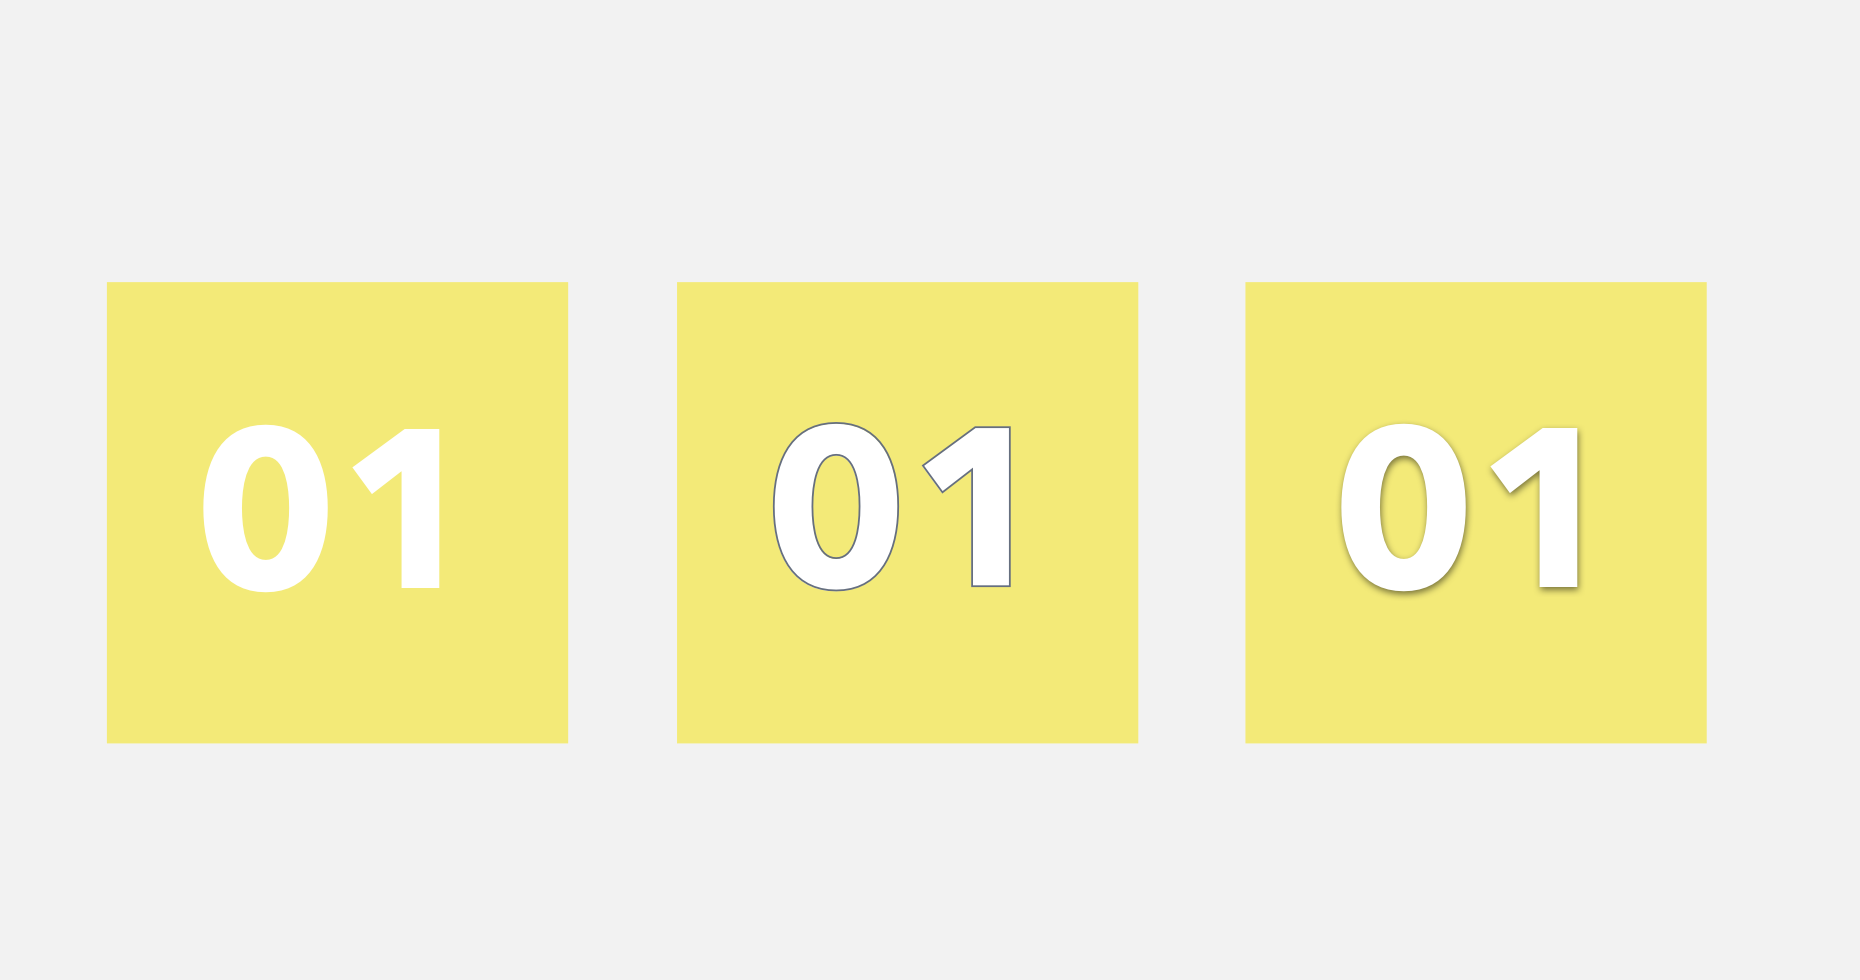
\includegraphics[width=\textwidth]{figures/something}
    \caption[Fargekontrast]{Eksempel på tiltak til hvordan synliggjøre hvit tekst på gul/oransje bakgrunn
    \label{fig:color_contrast}}
\end{figure}

Selve layouten har vi forholdt oss til en utforming som er godt kjent for de fleste med et konsistent design hvor vi følger normen for hvordan apper ser ut i dag og hvordan verktøyene allerede har predefinerte maler for hvordan layoutet skal se ut. For eksempel er hovedmenyen i bunn og hamburgermeny på topp. Vi har forholdt oss til hvordan appen til Kolonial ser ut i dag, men har byttet ut noen valg for å få tilpasset appen til å passe inn med vårt konsept.

Tilbakemeldinger til brukeren på utførte handlinger kommer ofte i en “Toast”. Denne dukker opp som en boks nederst på siden og er slik som det er på veldig mange apper. Vi skulle ønske at noen av disse kom bedre innenfor synsfeltet hvor brukeren har oppmerksomheten, men siden dette er en standard, og den har farger og bevegelser så har vi ikke gjort noe med dette. Det ville også føre til betydelig ekstraarbeid som vi ikke ville ha hatt tid til i disse iterasjonene.

%%%%%%%%%%%%%%%%%%%%%%%% LOGIN %%%%%%%%%%%%%%%%%%%%%%%% 
\subsection{\textbf{Innlogging}}
\begin{figure}[H]
    \includegraphics[width=\textwidth]{figures/teknisk/login/login}
    \caption[Innlogging 1]{Innloggingsside
    \label{fig:login}}
\end{figure}

\subsubsection{\textbf{Funksjonelt}}
Innloggingssiden brukes for å enten logge inn i appen, eller for å registrere seg. For å logge inn må brukeren ha en eksisterende konto hos Kolonial.no. Hvis brukeren ikke har det, så kan en ny bruker registreres ved å trykke på <<... Registrer deg her!>>. Grunnet mangel på endpoint for registrering hos Kolonial.no blir brukeren videresendt til deres egen registreringsside i en intern nettleser. 

Når bruker logger inn med sin påloggingsinformasjon fra Kolonial.no, sendes det en forespørsel til vår Firebase database for å se om vi har en lokal kopi av brukeren. Hvis vi ikke har en kopi av brukeren, så blir det opprettet en forespørsel til Kolonial.no sitt API for å autentisere bruker og få tilbake noe data om brukeren. Informasjonen vi får tilbake blir lagret i en Firebase kolleksjon. Neste gang bruker logger inn, så eksisterer det en lokal kopi i vår database og vi slipper å gjøre en forespørsel mot Kolonial.no sitt API. Vi mellomlagrer brukerdata for å kunne lagre favorittoppskrifter og beholdning til brukeren. Vi har ikke tatt hensyn til personvernforordningen GDPR (General Data Protection Regulation) siden appen skal fungere som en videreutvikling av deres eksisterende løsning. Vi forutsetter derfor at Kolonial.no følger de nye personvernsreglene.

\begin{figure}[H]
    \includegraphics[width=\textwidth]{figures/teknisk/login/users}
    \caption[Innlogging 2]{Dette er hvordan brukerinformasjon lagres hos oss. Vi lagrer det som returneres av API-et.
    \label{fig:userdb}}
\end{figure}

\subsubsection{\textbf{Visuelt}}
På siden for innlogging hadde vi opprinnelig en oransje farge som bakgrunnsfarge på prototypene. Vi valgte denne da dette var en farge vi hadde sett i Kolonial.nos opprinnelige løsning, og vi tenkte at konsistent design var å foretrekke. Dette gjorde vi selv om vi var under oppfatningen av at det strider med prinsipp for universell utforming, kontrast, og fargebruk. Oransje med hvit tekst gir ikke ideell synlighet. Dette endret vi på etter vi hadde hatt veiledning med produkteier. Vi endret til mer nøytrale og stilrene farger. Vi gikk for en grønnfarge vi tidligere hadde sett i Kolonial.nos løsning. 

Før du logger inn og trykker på feltene er feltene hvite med en grå understrek. Når du har fylt ut en gyldig epostadresse blir streken grønn samtidig som streken til feltet for passord blir oransje for å hinte til neste steg for brukeren. Ved feil inntasting blir streken rød under det feltet det gjelder. Vi har brukt farger som fungerer for de fleste, selv om man er fargeblind.

Knappen for å logge inn er satt filter på for å få ned kontrasten slik at når brukernavn og passord er fylt ut så blir knappen tydeliggjort med sterk kontrast, og viser at du er klar til å logge inn. Dette hjelper brukeren til å ikke gjøre feil, forstå og få tilbakemelding hva som skjer og hva brukeren har gjort.


%%%%%%%%%%%%%%%%%%%%%%%% HJEM %%%%%%%%%%%%%%%%%%%%%%%% 
\subsection{\textbf{Hjem og strekkodeleser}}
\begin{figure}[H]
    \includegraphics[width=\textwidth]{figures/teknisk/login/hjem}
    \caption[Hjem]{Hjemside [t.v] og strekkodeleser [t.h]
    \label{fig:hjem}}
\end{figure}

\subsubsection{\textbf{Funksjonelt}}
Hjemsiden er statisk og bare en visuell representasjon av deres eksisterende løsning.
I toppmenyen, øverst til venstre har vi strekkodeleser slik at man raskt og lett kan finne et produkt. Øverst til høyre har vi en hamburgermeny for å få aksessert brukerinnstillinger og logg ut-knapp.

\subsubsection{\textbf{Visuelt}}
Forsiden er bare et eksempel på layout, og ikke lagt mye vekt på da dagens kolonial.nos hjemmeside skal brukes ved en implementering. Med tanke på at oppskrifter er en stor del av vår idé så har vi valgt å ta med det på forsiden, som en ukemeny.

\subsection{\textbf{Strekkodeleser}}
\subsubsection{\textbf{Funksjonelt}}
Når man klikker seg inn på barcode scanneren øverst i venstre hjørne på hjem siden, kommer opp bilde 1. Her plasserer man bare strekkoden slik at den er på linje med den røde linjen på kameraet. Når man har scannet varen kommer man rett inn på produktsiden for produktet. 

En av plussidene med at vi byttet til Ionic er at vi har tilgang til et større bibliotek med moduler. Strekkodeleser er en modul som allerede eksisterer for Cordova, noe som betydde at vi slapp å implementere dette selv og dermed sparte mye tid på det. Cordova er mellomlaget mellom Ionic og telefonen, som lar oss ta i bruk funksjoner vi ellers ikke hadde hatt tilgang til (eks: kamera). Når bruker trykker på strekkoden på bilde 1, så blir det sendt en forespørsel til denne modulen som da starter opp kamera. Når en strekkode har blitt lest, så blir verdien på strekkoden returnert tilbake. Denne verdien bruker vi for å gjøre et søk i produktdatabasen til Kolonial.no, ved hjelp av deres API. Hvis produktet finnes i databasen deres, blir brukeren sendt videre til produktet. Hvis produktet ikke finnes, får bruker en melding om at dette er en vare som ikke er tilgjengelig.

\subsection{\textbf{Visuelt}}
På figuren ~\ref{fig:hjem} til høyre har vi strekkodeleser. Vi har prøvd å lage et ikon som passer overrens med resten av utforming på siden, samtidig som vi ønsker at brukeren skal gjenkjenne ikonet. Se produktside (\ref{sec:produkt}) for mer.

%%%%%%%%%%%%%%%%%%%%%%%% SØK %%%%%%%%%%%%%%%%%%%%%%%% 
\subsection{\textbf{Søk}}
\begin{figure}[H]
    \includegraphics[width=\textwidth]{figures/teknisk/sok/sok}
    \caption[Søkside]{Søkside
    \label{fig:sok}}
\end{figure}

\subsubsection{\textbf{Funksjonelt}}
Siden lar bruker søke gjennom varer i produktdatabasen til Kolonial.no. 
For hver endring i søkelinjen, blir det gjort en forespørsel mot Kolonial.no sitt API som returnerer en liste over produktene den finner med gitte søkekriterier. Vi begrenser antall resultater til 15, for å ta hensyn til databruk. Disse resultatene vil så bli presentert til brukeren (se figur \ref{fig:sok}).

\subsubsection{\textbf{Visuelt}}
Her har vi valgt å bruke sterke kontraster, ved å ha <<mørk>> som tekstfarge, mot hvit bakgrunn, samt utheve produktnavnet, og minske prisen. Da får vi størst blikkfang på produktbilde- og navn. 

%%%%%%%%%%%%%%%%%%%%%%%% PRODUKT %%%%%%%%%%%%%%%%%%%%%%%% 
\subsection{\textbf{Produkt}}
\label{sec:produkt}
\begin{figure}[H]
    \includegraphics[width=\textwidth]{figures/teknisk/produkt/produkt}
    \caption[Produkt]{Produktside
    \label{fig:produkt}}
\end{figure}

\textbf{Funksjonelt:}
Her kan du flytte produktet mellom kategorier i din beholdning, ved å klikke på - og +. Når bruker har gjort endringene sine og navigerer ut av siden, blir det gjort en forespørsel mot Firebase databasen om å lagre endringene bruker har gjort. Mer om hvordan databasen for total i beholdning og enkeltkategorier er satt opp kan leses om i \ref{sec:beholdning}

\textbf{Visuelt:}
Vi støtter på en logisk brist i visning av varer. Vi kom fram til at vi hadde tre forskjellige visninger av varer:\newline
1. Når man scanner en vare.\newline
2. Når man skal se på varen.\newline
3. Når man skal flytte og kjøpe varen.\newline 

Dette så vi først når vi begynte å bygge applikasjonen, selv etter tre prototyper og brukertesting.

Grunnen til at vi ikke så denne logiske bristen kan ha hatt en sammenheng med at vi har tenkt at Kolonial.no allerede har disse løsningene og at vi dermed ikke trengte å tenke på det. Vi ble klar over at vi ikke kunne vise en vare uten at kjøpknappen er til stede.

Med bakgrunn i dette tok vi en runde på tavlen og fikk tegnet opp alle varianter av mulige visninger av en vare og hvordan man navigerer dit. Med denne prosessen så vi at dette kunne være en visning som kunne være overalt uavhengig om man går inn på en vare i beholdning eller scanner en vare. 

Dette gir fordeler for brukeren ved at de kun trenger å forholde seg til en type side. 

Vi så fort at det kom til å bli mye informasjon på visningen av en vare og måtte kutte eller sørge for at bruker ikke ble presentert med all informasjon om en vare på en gang. Løsningen vi kom frem til var en liste med informasjon om varen og beholdning.

%%%%%%%%%%%%%%%%%%%%%%%% OPPSKRIFTER %%%%%%%%%%%%%%%%%%%%%%%% 
\subsection{\textbf{Oppskrifter}}
\begin{figure}[H]
    \includegraphics[width=\textwidth]{figures/teknisk/oppskrifter/oppskrifter}
    \caption[Oppskrifter]{Oppskrifterside
    \label{fig:oppskrifter}}
\end{figure}

\subsubsection{\textbf{Funksjonelt}}
Oppskrift siden er bygd opp slik at man kan få forslag til hva man skal ha til middag. Øverst har man fire forskjellige kategorier man kan velge mellom.

\textbf{Populære:}
\\Inne på denne kategorien ligger de oppskriftene som har fått flest favoritter fra brukere. Hvor populær en vare er blir sporet ved å ha ett <<integer>-felt i oppskriften, som økes og reduseres når en bruker legger til eller fjerner oppskriften fra sine favoritter.

\textbf{Favoritter:}
\\Når man er inne på en oppskrift har man mulighet til å legge oppskriften inn i favoritter, som best passer din beholdning, og legges da inn her. Hvilke oppskrifter en bruker har favorisert blir lagret i en kolleksjon <<favorites>>, som er en subkolleksjon av bruker-dokumentet (se figur \ref{fig:userdb}).

\textbf{Dine varer:}
\\Dine varer er basert på varene man har lagt inn i sin beholdning. Øverst i venstre hjørnet står det hvor stor andel av varene man har i beholdningen. Dette tallet regnes ut ved å sammenligne varene som bruker har i beholdning, med varer som oppskriften trenger. Basisvarer blir ikke tatt med når match blir regnet ut.

\textbf{Pris:}
\\Er sortert etter hvilke retter som er billigst. Pris blir regnet ut ved å ta i betraktning hva bruker allerede har, slik at kun varene bruker mangler blir summert i pris.

\begin{figure}[!h]
    \includegraphics[width=\textwidth]{figures/teknisk/oppskrifter/oppskrifterdb}
    \caption[Oppskrifter - Databasestruktur]{Databasestruktur for oppskrifter
    \label{fig:oppskrifterdb}}
\end{figure}

\newpage
\textbf{Visuelt:}
Denne siden finnes allerede hos Kolonial.no. På den eksisterende er det to oppskrifter i bredden, mens vi har valgt å ha én oppskrift i bredden. Dette for å ha fokus på én oppskrift av gangen. Dette gir større plass til bilde slik at brukeren skal se retten/oppskriften bedre og bli fristet. Vi har også lagt til en knapp for å gjøre det mer intuitivt å klikke på oppskriften.

På bildet av oppskrifter basert på beholdning har vi en visuell fremstilling av hvor stor prosentdel av oppskriften bruker har i beholdning. I prototypen kan denne bytte farge med andelen av prosentsats. Dette vil si at om man har alle ingrediensene til en oppskrift, eller mer, så er dette feltet grønt med 100 \%.

Vi har brukt <<primær>> som farge for en aktiv kategori og knapp for å
skape blikkfang. I tillegg bruker vi <<mørk>> som farge på tekst mot hvit bakgrunn
for å ta hensyn til universell utforming.


%%%%%%%%%%%%%%%%%%%%%%%% ENKELTOPPSKRIFT %%%%%%%%%%%%%%%%%%%%%%%% 
\subsection{\textbf{Enkeltoppskrift}}
\begin{figure}[H]
    \includegraphics[width=\textwidth]{figures/teknisk/oppskrifter/oppskrift}
    \caption[Oppskrift]{Side for oppskrift
    \label{fig:oppskrift}}
\end{figure}

\textbf{Funksjonelt:}
I oppskriften ser man en liste over ingredienser, og hvor mange man trenger av hver. Her kan man justere porsjoner med pluss- og minus-tegnene. Når man legger til og trekker fra porsjoner endres også volumet av ingrediensene man trenger. Dersom varen er en basisvare, som f.eks. krydder eller vann vil det stå <<BASIS>> fremfor mengde. Dersom man likevel trenger basisvaren kan man trykke seg inn til produktsiden og kjøpe derifra. I en ferdig løsning ville vi hentet ut oppskrifter fra API-et deres, men grunnet vår ekstrafunksjonalitet som <<Oppskrifter basert på beholdning>> får vi ikke ut all informasjon vi trenger. Vi har derfor valgt å lage noen <<dummy>>-oppskrifter for å vise hvordan det ville fungert i en vanlig løsning.

\subsubsection{\textbf{Bruk Oppskrift:}}
Denne knappen vil trekke fra alle varene som brukes i oppskrifter fra beholdningen din, og regne ut riktig mengde. Dette gjør det mulig å bruke f.eks. 1/3 av en hel ost fremfor at hele produktet fjernes fra beholdning. 

\subsubsection{\textbf{Kjøp: }}
Vi har kuttet hele kjøpsprosessen ettersom den allerede finnes i den eksisterende løsningen. Vi valgte å gjøre det slik at produktene du <<kjøper>>, automatisk blir lagt til usortert i beholdningen.

\subsubsection{\textbf{Favoritt: }}
Øverst i høyre hjørne finner du et hjerteikon som tillatter brukeren å favorisere en oppskrift. Dette vil øke oppskriftens rangering i <<Populære>>-kategorien, samt legge oppskrifter til i <<Favoritter>>-kategorien.

\newpage
\textbf{Visuelt:}
Fargevalgene vi endte opp med var:\newline
<<pris>>: Grå bakgrunn på basisvarer for å ikke ta unødig stor oppmerksomhet.\newline
<<bringebær>>: Dersom brukeren mangler varer ville det være uthevet i en rødfarge for å skape kontrast og få stor oppmerksomhet.\newline
<<grønn>>: Tilsvarende bringebær brukes grønnfargen for å fange oppmerksomhet, og grønn oppleves som en farge for at noe er <<riktig>>. Det representerer at brukeren har nok av en vare.

%%%%%%%%%%%%%%%%%%%%%%%% BEHOLDNING %%%%%%%%%%%%%%%%%%%%%%%% 
\subsection{\textbf{Beholdning}}\label{sec:beholdning}
\begin{figure}[H]
    \includegraphics[width=\textwidth]{figures/teknisk/beholdning/beholdning}
    \caption[Beholdning]{Beholdningsside
    \label{fig:beholdning}}
\end{figure}

\textbf{Funksjonelt:}
På beholdningssiden ser man alle varene man har lagt til i beholdning. Dersom man ikke
manuelt sorterer varer vil det legges til i usortert. Man kan velge hvor mange av en vare man har, og det vil slettes automatisk dersom antallet er 0.

\begin{figure}[H]
    \includegraphics[width=\textwidth]{figures/teknisk/beholdning/beholdningdb}
    \caption[Beholdning - Database]{Referansen til en kategori i databasen ser slik ut: storage/{brukerId}/{kategoriId}.
Tallene 0-4 i kolleksjonen referer til en spesifikk kategori. Innenfor kategorien blir produktet lagret med produkt id som dokument id. Kolleksjonen quantity inneholder et dokument med produkt id som dokument id, og dette dokumentet har et felt ‘total’ som holder telling på totalsummen av produktet brukeren har.
    \label{fig:beholdningdb}}
\end{figure}

\textbf{Visuelt:}
Øverst har vi et søkefelt for å fort finne ønsket produkt.
Under har vi kategorier for å lettere ha oversikt over hvor diverse produkter befinner seg. Så blir produktene brukeren har i beholdningen listet nedover med oversikt over hvor mye av produktet du har igjen.

%%%%%%%%%%%%%%%%%%%% DESCRIPTION %%%%%%%%%%%%%%%%%
\section{\textbf{Installasjon av løsning}}
\subsection{\textbf{Brukerinformasjon}}
1. Brukernavn: gruppe16smidig@gmail.com\\
2. Passord   : Kolonial123\\
$\rightarrow$ Eventuelt egen bruker hos Kolonial.no

\subsection{\textbf{Google Play Store}}
Løsningen er tilgjenglig på Google Play Store for Android-enheter.
\url{https://play.google.com/store/apps/details?id=no.octopod.smidig.kolonial}

\subsection{\textbf{Forkrav for bygging av prosjekt}}
Det forutsettes at Cordova, Ionic og Node er installert for å kunne bygge løsningen selv.

\subsubsection{\textbf{Installering av forkrav}}
\paragraph{\textbf{Node}}
\subparagraph{Windows}
Node for Windows kan lastes ned fra \url{https://nodejs.org/en/download/}.

\subparagraph{MacOS}
Installer Node med cURL:
\begin{minted}[breaklines]{bash}
curl "https://nodejs.org/dist/latest/node-${VERSION:-$(wget -qO- https://nodejs.org/dist/latest/ | sed -nE 's|.>node-(.).pkg.*|\1|p')}.pkg" > "$HOME/Downloads/node-latest.pkg" && sudo installer -store -pkg "$HOME/Downloads/node-latest.pkg" -target "/"
\end{minted}

\subparagraph{Linux}
\begin{minted}[breaklines]{bash}
curl -sL https://deb.nodesource.com/setup_8.x | sudo -E bash - sudo apt-get install -y nodejs
\end{minted}

\paragraph{\textbf{Ionic og Cordova}}
\paragraph{Windows, MacOS og Linux\newline}
Kjør følgende kommando i terminalvinduet:
\begin{minted}[breaklines]{bash}
npm install -g ionic cordova
\end{minted}

\subsection{\textbf{Kjøre løsningen}}
Kildekoden for løsningen kan lastes ned fra \url{https://github.com/Westerdals/PRO200-17-16/archive/master.zip}.

\subsubsection{\textbf{Kjør på Android}}
Android SDK og Java JDK er forkrav for å kunne bygge APK for Android.
Android SDK kan lastes ned fra \url{https://developer.android.com/studio/}.
Java JDK kan lastes ned fra \url{http://www.oracle.com/technetwork/java/javase/downloads}.

Koble til telefonen og kjør følgende kommando i rotmappen til løsningen:
\begin{minted}[breaklines]{bash}
ionic cordova run android
\end{minted}

\textit{Løsningen kan også kjøres i Android Emulator ved å kjøre samme kommando uten å koble til telefon.}

\subsubsection{\textbf{Emulering i nettleser}}
\textit{Å kjøre løsningen i web er ikke anbefalt. Applikasjonen fungerer ikke som tiltenkt, grunnet CORS-restriksjoner i Kolonials API}.

Kjør følgende kommando i rotmappen til løsningen:
\begin{minted}[breaklines]{bash}
ionic serve --lab
\end{minted}
\textbf{NB! CORS må skrus av for å kunne kjøre løsningen i nettleser!}

\paragraph{\textbf{Deaktiver CORS i Google Chrome}}\mbox{}
\subparagraph{{Windows}}\mbox{}\\
1. Lukk alle Chrome-vinduer\\
2. Kjør følgende kommando i mappen chrome er installert i:
\begin{minted}[breaklines]{bash}
chrome.exe --disable-web-security --user-data-dir
\end{minted}

\subparagraph{{MacOS}}\mbox{}\\
1. Lukk alle Chrome-vinduer\\
2. Kjør følgende kommando i terminalvindu:
\begin{minted}[breaklines]{bash}
open -a Google\ Chrome --args --disable-web-security --user-data-dir
\end{minted}

\subparagraph{{Linux}}\mbox{}\\
1. Lukk alle Chrome-vinduer\\
2. Kjør følgende kommando i terminalvindu:
\begin{minted}[breaklines]{bash}
google-chrome --disable-web-security --user-data-dir
\end{minted}

\paragraph{\textbf{Deaktiver CORS i Safari}}\mbox{}\\
1. Aktiver Developer Tools in Safari\\
2. Develop $\rightarrow$ Disable Cross-Origin Restrictions


%\chapter{Kommunikasjonsstrategi}
\section{\textbf{Lojalitetshjul}} 
En grafisk og funksjonell fremstilling av brukers reise fra \textit{kjennskap} (laveste rangering for hvor lojal en bruker kan være til merkevaren) til \textit{disippel} (høyeste rangering for hvor lojal en bruker kan være til merkevaren), på bakgrunn av Digital Involvement Cycle-modellene (se figur \ref{fig:digitalcycle}), for å sikre fremdrift i brukerfasene og økt Customer Lifetime Value (CLV). 

\begin{figure}[H] 
    \centering
    \includegraphics[width=\textwidth]{figures/komstrat/digitalcycle.png}
    \caption[Digital Involvement Cycle-modell]{Digital Involvement Cycle-modell. Til venstre ser man de forskjellige fasene en bruker går gjennom, forklart i mål for bruker for hver fase i inndelingen for mål. På toppen inndeling for hva som skal oppnås gjennom hver fase. Se vedlegg \ref{vedlegg:1} og \ref{vedlegg:2} for ferdig utfylt modell for hver av målgruppene.
    \label{fig:digitalcycle}}
\end{figure}

CLV beskriver hvor mye profitt du kan forvente å få ut av bruker gjennom kundeforholdet (Artun og Levin 2015, 64). Brukere kan i denne sammenheng sees på som aksjer, noen er verdt mer enn andre, og verdien kan endres gjennom kundeforholdet (Artun og Levin, 10). <<Bruker>> refererer til en person som benytter løsningen og handler hos Kolonial.no.

Hjulene (figur \ref{fig:lojalpersona1} og figur \ref{fig:lojalpersona2}) er smidig utformet for å lett tilpasse endringer gjennom brukerfasene, på bakgrunn av kontinuerlige målinger. De er bygget slik at man skal kunne hoppe inn i hvilken som helst fase, og jobbe uten å ha lest gjennom hele strategien.

\paragraph{\textbf{Login til Plandisc hvor hjulene kan sees i detalj:}} \\\url{https://create.plandisc.com/wheel/list}
\\Brukernavn: clesig16@student.westerdals.no 
\\Passord: SigneogEmilie2018

\begin{figure}[H] 
    \centering
    \includegraphics[width=\textwidth]{figures/komstrat/Lojalitetshjul1}
    \caption[Lojalitetshjul - persona 1]{Lojalitethjul for persona 1. Forklart nærmere i kapittel \ref{sec:persona1}.
    \label{fig:lojalpersona1}}
\end{figure}

\begin{figure}[H] 
    \centering
    \includegraphics[width=\textwidth]{figures/komstrat/Lojalitetshjul2}
    \caption[Lojalitetshjul - persona 2]{Lojalitethjul for persona 2. Forklart nærmere i kapittel \ref{sec:persona2}).
    \label{fig:lojalpersona2}}
\end{figure}

Den ytterste ringen er delt i 7, og beskriver fasen aktivitetene er planlagt å målrettes til. Den midterste ringen beskriver aktivitetene som er planlagt, hvor hver aktivitet er fargekodet for å lettere få oversikt over hvor ofte en aktivitet skal gjennomføres. Den innerste ringen er en oversikt over målingene som må gjøres for å aktivt drive optimalisering av innholdet. 

Aktivitetene i hver fase vil naturlig kjøre mer eller mindre parallelt, da brukere alltid vil være på forskjellige steder i involveringssyklusen, og samtidig krever spesialtilpasset innhold. Noen aktiviteter som er satt i en fase vil også kunne sees av brukere i andre faser, enda innholdet er rettet til fasen det er satt i. Fasene er ikke basert på tid i form av måneder og dager, men hvor lenge hver enkel bruker er i hver enkel fase, noe som alltid vil være relativt da tid i hver fase vil variere fra bruker til bruker.

Forbrukere blir mer og mer opptatt av hverandres meninger, og deler disse i stor grad på sosiale medier. Sammen danner de et bilde av produkt eller bedrift, som ofte er svært forskjellig fra slik bedriften mener å fremstå (Kotler, m.fl. 2017, 13). Derfor er er strategien lagt opp slik at Kolonial.no hele tiden viser sin tilstedeværelse, for å møte både nåværende og potensielle brukere, og aktivt være i dialog for å fremstå og skape det bildet de ønsker bruker skal ha.

Brukere blir overøst av kommunikasjon hver dag hele tiden, som ofte oppfattes som svært upersonlig da det går ut til mange brukere samtidig, og det krever derfor en mer personlig tilnærming om bruker skal interagere med kommunikasjonen (Artun og Levin 2015, 3 og 14). Bedrifter må bli synlig i mengden, og kommunisere på en måte som er meningsfull for bruker. For å klare dette bør bedriften kartlegge kundereisen, fra første interaksjon med bedrift/løsning, til konvertering, og videre kundeforhold, for å virkelig forstå de forskjellige stadiene. De bør fokusere på hvem som mottar hvilken kommunikasjon, når (Kotler, m.fl. 2017, 59).

Bruker skal føle seg sett og ivaretatt, og vil med det bruke mer tid og penger på merkevaren. Hvis vi gir verdi, vil vi få verdi tilbake (Artun og Levin, 3). Det er derfor viktig å ta høyde for at det alltid vil være endringer i bruksmønster, og teknologiske løsninger, slik at brukers ønsker, behov og verdier møtes. Hjulet er utformet smidig, nettopp for at man skal kunne gjøre disse justeringene underveis.

Lojalitetshjulene er basert på <<Digital Involvement Cycle>>-analysene. Disse analysene reflekterer hvordan merkevaren interagerer med målgruppene gjennom kundereisen. Brukerne interagerer med forskjellige touch points ettersom de beveger seg gjennom de ulike fasene i hjulene. Brukerne kan starte i hvilken som helst fase, avhengig av hvor godt kjent de er med Kolonial.no og løsningen fra før av (Kaufman og Horton 2015, 118-119).



\subsection{\textbf{Persona 1}}
\label{sec:persona1}
Se figur \ref{fig:persona1}

\subsubsection{\textbf{Fase 1: Opplyst - Kjennskap Top of Mind 5}}
I fase 1 skal vi fokusere på at forbrukeren skal kjenne til Kolonial.no som bedrift. Målet med fasen er at forbrukeren skal ha Kolonial.no på sin <<Top of Mind 5>>-liste av dagligvarehandelforretninger. Bruker skal vite at Kolonial.no eksisterer og at det er en dagligvarehandel på nettet.

\textbf{Facebook ads:} På Facebook vil det publiseres segmenterte annonser som inneholder budskap som omhandler Kolonial.no som bedrift og at de er grønne, som vil engasjere vår persona. I denne aktiviteten er målet  å skape en kjennskap til Kolonial.no. 

\textit{Måling:} For å måle i hvor stor grad dette skaper interesse, og dermed kjennskap, vil vi legge en sporingslenke/Facebook Pixel som en CTA som vil måle clickraten til nettbutikken. En Facebook Pixel er en HTML-kodesnutt som hjelper oss å måle. Den vil i dette tilfelle måle hvor mange som trykker seg inn på linken, og videre til nettbutikken (Faizi 2017). 

\textbf{Instagram ads:} På Instagram vil det publiseres rettede annonser via Facebook Manager (Facebooks eget annonseverktøy), da Manager innehar bedre segmenteringsmuligheter enn Instagram, kontoene må da være linket sammen gjennom Facebook. 

Disse annonsene vil ha samme tema som Facebook: introduksjon til Kolonial.no, med fokus på at de er grønne. 

\textit{Måling:} For å måle i hvor stor grad dette skaper interesse, og dermed kjennskap, vil vi legge en sporingslenke som en CTA som vil måle clickraten til hjemmesiden. 

\textbf{Nettaviser:} På nettavisene vil det være reklame både i form av banner og video, og disse vil veksle: en uke banner - en uke video. Med banner mener vi vanlige reklamebannere man får opp når man scroller på nettaviser, med video så mener vi en kort reklamesnutt foran videoene på for eksempel VGTV eller DBTV. Disse vil jobbe med å introdusere Kolonial.no og øke kjennskapen. 

Handlingen i reklamefilmen skal omhandle miljø, og hvor lett det er å minske matsvinnet i sitt eget hjem. Det kan være at personen i filmen skal til å lage pizza, men får en notification på mobilen om at melken går ut på dato snart. Personen begynner å lage grøt i stedet for. Vi vil vise hvor enkelt løsningen sier i fra. 

\textit{Måling:} For å måle dette vil vi legge en sporingslenke som en CTA som vil måle clickraten til hjemmesiden. 

\textbf{For å måle målet:} For å spesifikt måle <<Top of Mind 5>> vil vi utføre spørreundersøkelser gjennom Norstat/Gallup for å se hvor brukerne måtte befinne seg.

\subsubsection{\textbf{Fase 2: Interesse}}
I fase 2 skal vi fokusere på at forbrukeren skal bli interessert og nysgjerrig på Kolonial.no som merkevare. Målet med fasen er at forbrukeren skal ha Kolonial.no på sin <<Top of Mind 3>>-liste av dagligvarehandel. Vi vil at personaen skal vite at Kolonial.no er en miljøbevisst og grønn matvarehandel, da dette er faktorer som vil appellere til målgruppen. 

\textbf{Facebook organisk:} Her vil vi publisere segmenterte annonser som inneholder budskap som vil engasjere vår persona: matsvinn, miljø og at bedriften er grønn. I denne aktiviteten er det altså fokus på å skape interesse for Kolonial.no. Dette vil postes ut 1 gang i uka. 

For å måle i hvor stor grad dette skaper interesse vil vi legge en sporingslenke/Facebook Pixel som en Call-To-Action som vil måle clickraten til nettbutikken. Vi vil også se på engasjement i form av likes, delinger og kommentarer for å se interessen.

\textit{Måling:} For å måle dette vil vi legge en sporingslenke/Facebook Pixel som en Call-To-Action som vil måle clickraten til nettbutikken. 

\textbf{Instagram organisk:} Det vil legges ut segmenterte annonser på Instagram via Facebook Manager, da Manager innehar bedre segmenteringsmuligheter enn Instagram, kontoene må da være linket sammen via Facebook. Vi vil fokusere på innhold som omhandler matsvinn og at Kolonial.no er en grønn bedrift. Dette vil postes 1 gang i uka. 

\textit{Måling:} For å måle dette vil vi legge en sporingslenke som en CTA som vil måle clickraten til hjemmesiden. 

\textbf{Utendørs:} Vi vil ha reklameplakater på Adshells ved bysykkelstativ, i tillegg til på bysyklene. Disse reklamene skal fremme Kolonial.no som en grønn miljøbevisst matvarehandel på nett. Bysyklene er relevante da det er kollektiv transport og målgruppen vår er miljøbevisst. Miljøvennlige løsninger passer midt i blinken for vår målgruppe. Dette vil pågå hele sesongen. 

\textit{Måling:} For å spesifikt måle <<Top of Mind 3>> vil vi utføre spørreundersøkelser gjennom Norstat/Gallup for å se hvor brukerne måtte befinne seg. 

\textbf{Blogg:} Kolonial.no har allerede en eksisterende blogg som per dags dato ikke er veldig aktiv. En fin måte å spre kunnskap og å skape verdi for brukeren på er å bruke dette som en kanal. Det vil her postes innlegg med grønne tips og triks, oppskrifter, og også hvordan/hvorfor bedriften Kolonial.no er grønne. 

Eksempel: <<Hva gjør vi for å sørge for at bananene våre har en grønn utvikling>>. 

Blogginnleggene vil bli sendt ut på både Facebook og nyhetsbrev. Det vil postes 1 gang i uka. På blogginnleggene vil det også ligge en mulighet for å registrere seg på nyhetsbrev for å få mer informasjon, tips og triks og oppskrifter. 

\textit{Måling:} Når det kommer til måling vil det sees på hvor mange som er inne, hvor lenge, hvor de kommer fra. Vi vil også se på hvor mange som er registrert vs hvor mange som åpner opp nyhetsbrevet. Dette er for å måle interessen. 

\textbf{Nyhetsbrev:} Det er ingen nyhetsbrev spesifikke for denne fasen, men man vil via blogginnlegget kunne registrere seg på nyhetsbrevet.

\subsubsection{\textbf{Fase 3: Involvert}}
I fase 3 er målet at bruker skal laste ned appen, og registrere bruker. Bruker skal vite at appen ikke bare har som hensikt å selge, men også være med på å bekjempe matsvinn i hjemmet ved bruk av <<oppskrift basert på beholdning>>-funksjonen. Kolonial.no bekjemper også matsvinn innad i bedriften, og dette gjør at Kolonial.no er en bedrift som gjør handling ut av ord. 


\textbf{Facebook ads:} Det vil legges ut et innlegg som tilbyr nye bruker et velkomsttilbud på 200 kr avslag på første bestilling. Dette vil være med på å sikre at de som er interesserte laster ned og tester løsningen, og kanskje senere blir faste brukere. 

\textit{Måling:} For å måle dette vil vi legge en sporingslenke som en CTA som vil måle clickraten til nettbutikken. Vi vil også se hvor mange som har lastet ned appen, og brukt tilbudet. 

\textbf{Organisk Facebook:} Her vil vi publisere segmenterte annonser som inneholder budskap som vil engasjere vår persona: matsvinn, miljø og at bedriften er grønn. Vi vil også poste blogginnlegg via poster på Facebook. I denne aktiviteten er det altså fokus på å skape interesse for Kolonial.no. Dette vil postes ut 1 gang i uka. 

\textit{Måling:} For å måle dette vil vi legge en sporingslenke/Facebook Pixel som en CTA som vil måle clickraten til hjemmesiden. Vi vil også se på engasjement i form av likes, delinger og kommentarer for å se interessen.  

\textbf{Organisk Instagram:} Det vil legges ut segmenterte annonser på Instagram via Facebook Manager, da Manager innehar bedre segmenteringsmuligheter enn Instagram, kontoene må da være linket sammen via Facebook. Vi vil fokusere på innhold som omhandler matsvinn og at Kolonial.no er en grønn bedrift. Postes 1 gang i uka. 

\textit{Måling:} For å måle dette vil vi legge en sporingslenke som en CTA som vil måle clickraten til nettbutikken. Vi vil også se på engasjement i form av likes, delinger og kommentarer for å se interessen. 

\textbf{Nyhetsbrev:} Vi sender ut nyhetsbrev som er målrettet til persona 1. Det vil være alt fra inspirasjon til matretter, hvordan du skal bruke opp maten hjemme: <<Hva kan du bruke den utgåtte melka til?>>, oppskrifter basert på den enkeltes beholdning og oppskrifter til dette. Det er også her en del av blogginnleggene vil bli sendt ut. Mailene og blogginnleggene vil også reklamere for appen, og vise frem Middagsassistenten. Det vil bli sendt ut 2 ganger i uka. 

\textit{Måling:} For å måle målet <<Laste ned app og registrere bruker>> ser vi på nedlastningstallene for appen, og sammenligner med hvor mange som faktisk har registrert seg. 

\subsubsection{\textbf{Fase 4: Forpliktelse/konvertering}}
I fase 4 er målet at forbrukeren skal bruke appen av og til - at det skal være noe de vurderer  hver gang de handler. Bruker skal vite at appen ikke bare har som hensikt å selge, men også være med på å bekjempe matsvinn i hjemmet ved bruk av <<oppskrift basert på beholdning>>-funksjonen. Kolonial.no bekjemper også matsvinn innad i bedriften, og dette gjør at Kolonial.no er en bedrift som gjør handling ut av ord. Dette vil gi den miljøbevisste målgruppen en god grunn til å bruke Kolonial.no gjentatte ganger. 

Denne målgruppen vil se postene og blogginnleggene til fasene over, men i denne fasen vil det være fokus på notificationfunksjonen som forteller deg hvis du har en ubrukt vare i beholdning som holder på å gå ut på dato. 

\textbf{Notification:} Forbrukeren får en notification på mobil hvis det er en vare i beholdning som nærmer seg utløpsdato. For eksempel: <<Melken din holder på å gå ut på dato, hva med pannekaker?>>. Brukeren vil få et alternativ som passer til beholdningen, så langt det lar seg gjøre. Dette viser at Kolonial.no faktisk er opptatt av å minske matsvinn, leder til godt omdømme, i tillegg til at dette gagner brukeren. 

\textbf{Nyhetsbrev:} Hvis bruker ikke reagerer på notification og varen ikke er brukt innen 2 dager vil samme beskjed komme på e-post/nyhetsbrev. 

\textit{Måling:} For å måle dette vil det sees på hvor mange som åpner appen gjennom notification/e-post, om de utfører handlinger (bruker varen), eller om det gjøres nye kjøp. 

\subsubsection{\textbf{Fase 5: Lojalitet}}
I fase 5 skal det fokuseres på at forbrukeren skal bruke Kolonial.no og løsningen aktivt. Kolonial skal ligge på første plass på <<Top of Mind>>-listen, og være den foretrukne dagligvarehandleren. Bruker skal bruke middagsassistenten og beholdningsoversikten 7 av 10 ganger. 

\textbf{Facebook organisk:} I denne aktiviteten vil det fokuseres på resteoppskrifter og hvordan unngå matsvinn. Det vil postes innlegg på Facebook som oppfordrer til engasjement i form av likes, kommentarer og delinger. Det vil deles en <<resteoppskrift>>, og deretter oppfordres til at følgerne kan dele sine rester og tips til hva de kan brukes til. Det vil publiseres to innlegg i uka for denne fasen. 

\textit{Måling:} For å måle dette ser vi på engasjementet i form av likes, kommentarer og delinger. Vi vil også se på i hvor stor grad engasjementet i kommentarfeltet er relatert til det som det oppfordres til.

\textbf{Instagram organisk:} Det vil her brukes Instagram Stories for å sette fokus på matsvinn, dele andre brukeres bilder og oppskrifter. Alt vil foregå litt mer muntlig og lett her. Bildene fra brukere trenger ikke ha den beste kvaliteten for å bli delt. I tillegg til aktivitet på Stories vil det også være vanlige innlegg som omhandler matsvinn og resteoppskrifter: <<Se hva Tine gjorde med potetrestene sine!>>. Det vil være to faste dager i uka med Stories (i tillegg til ved behov, det skjer noe spesielt) og ett vanlig innlegg på Instagram i uka. 

\textit{Måling:} Dette vil måles via engasjement i form av likes, kommentarer, delinger og seere på Stories og vanlig innlegg. 

\textbf{Notification:} Forbrukeren får en notification på mobil hvis det er en vare i beholdning som nærmer seg utløpsdato. For eksempel: <<Melken din holder på å gå ut på dato, hva med pannekaker?>>. Brukeren vil få et alternativ som passer til beholdningen, så langt det lar seg gjøre. Dette viser at Kolonial.no faktisk er opptatt av å minske matsvinn, leder til godt omdømme, i tillegg til at dette gagner brukeren. 

\textit{Måling:} Dette måles ved å se på hvor mange åpner appen gjennom notification, og om det utføres handlinger (bruker varen).

\textbf{Nyhetsbrev:} Hvis bruker ikke reagerer på notification og varen ikke er brukt innen 2 dager vil samme beskjed komme på e-post/nyhetsbrev. 

For å måle dette vil det sees på hvor mange som åpner appen gjennom notification/e-post, om de utfører handlinger (bruker varen), eller om det gjøres nye kjøp, 

\textbf{\textit{For å måle målet:}} For å spesifikt måle <<Top of Mind 1>> vil vi utføre spørreundersøkelser gjennom Norstat/Gallup for å se hvor brukerne måtte befinne seg. 


\subsubsection{\textbf{Fase 6: Ambassadør}}
I fase 6 er ønsket at forbrukeren alltid bruker Kolonial.no, og foretrekker det foran alle de andre dagligvarehandlerne. Vi vil at forbrukeren skal bruke middagsassistenten og beholdningsoversikten 9 av 10 ganger. 

\textbf{Facebook organisk:} I denne aktiviteten vil det fokuseres på resteoppskrifter og hvordan unngå matsvinn. Det vil postes innlegg på Facebook som oppfordrer til engasjement i form av likes, kommentarer og delinger. Det vil deles en <<resteoppskrift>>, og deretter oppfordres til at følgerne kan dele sine rester og tips til hva de kan brukes til. Det vil publiseres to innlegg i uka for denne fasen. 

For å måle dette ser vi på engasjementet i form av likes, kommentarer og delinger. Vi vil også se på i hvor stor grad engasjementet i kommentarfeltet er relatert til det som det oppfordres til.

\textbf{Instagram ads:} Det vil, i likhet med Facebook, her fokuseres på resteoppskrifter og hvordan unngå matsvinn. Det vil deles ideer til resteoppskrifter, i tillegg til at man oppfordrer følgerne til å gjøre det samme. Det vil publiseres innlegg 1 gang i uka. 

For å måle dette ser vi på engasjementet i form av likes, kommentarer og delinger. 

\textbf{Notification:} Bruker får en notification på mobil hvis det er en vare i beholdningen som er ubrukt og som nærmer seg utløpstid. 

\textbf{Notification - SoLoMo:} SoLoMo er en forkortelse for Social Local Mobile. Ved bruk av SoLoMo kan vi tracke hvor bruker befinner seg. (Kaufman og Horton 2015, 53-55) Hvis bruker befinner seg i nærheten av et pick-up point, på samme tid som pick-up pointet har varer som snart går ut på dato, vil bruker få en notification på mobilen som gir den muligheten til å komme å kjøpe varer som snart utgår for en billigere penge. 

\textit{Måling:} For å måle dette vil vi se hvor mange som kom innom pick up-pointet i forhold til hvor mange som mottok notifications. 

\textbf{Nyhetsbrev:} Vi sender ut nyhetsbrev som er målrettet til persona 1. Det vil være alt fra inspirasjon til matretter, hvordan du skal bruke op maten hjemme: <<Hva kan du bruke den utgåtte melka til?>>, oppskrifter basert på den enkeltes beholdning og oppskrifter til dette. Det er også her en del av blogginnleggene vil bli sendt ut. 

\textit{Måling:} Hvis bruker ikke reagerer på notification og varen ikke er brukt innen 2 dager vil samme beskjed komme på e-post/nyhetsbrev. 

\subsubsection{\textbf{Fase 7: Disippel}}
I denne fasen er målet at brukeren skal føle en form for eierskap til løsningen. Brukeren skal være med på å spre budskapet, gjennom markedsføring som <<Friend of Mine>> og <<Word of Mouth>>. 


\textbf{Facebook ads:} På Facebook skal vi i denne fasen begynne å se etter engasjement og lojalitet. For å appellere mer til engasjementet om matsvinn vil det postes ideer til resteoppskrifter, og i tillegg legges ved en form for <<CTA>> som oppfordrer til aktivitet i kommentarfeltet: <<Hvilke rester må du bli kvitt i dag? Hva skal du lage med dine rester?>>. 

\textit{Måling:} For å måle dette ser vi på engasjementet i form av likes, kommentarer og delinger. Vi vil også se på i hvor stor grad engasjementet i kommentarfeltet er relatert til det som oppfordres. 

\textbf{Notification:} Bruker får en notification på mobil hvis det er en vare i beholdningen som er ubrukt og som nærmer seg utløpstid. 

\textit{Måling:} For å måle dette ser vi på hvor mange som åpnet appen via notification, og om du gjorde noen handlinger (bruker varen). 

\textbf{Notification - SoLoMo:} Ved bruk av SoLoMo kan vi tracke hvor bruker befinner seg (Kaufman og Horton 2015, 53-55). Hvis bruker befinner seg i nærheten av et pick-up point, på samme tid som pick-up pointet har varer som snart går ut på dato, vil bruker få en notification på mobilen som gir den muligheten til å komme å kjøpe varer som snart utgår for en billigere penge. 

\textit{Måling:} For å måle dette vil vi se hvor mange som kom innom pick up-pointet i forhold til hvor mange som mottok notificationen. 

\textbf{Nyhetsbrev:} Vi sender ut nyhetsbrev som er målrettet til persona 1. Det vil være alt fra inspirasjon til matretter, hvordan du skal bruke opp maten hjemme: <<Hva kan du bruke den utgåtte melka til?>>, oppskrifter basert på den enkeltes beholdning og oppskrifter til dette. Det er også her en del av nyhetsbrevene vil bli sendt ut. 

For å måle dette vil det sees på hvor mange som åpner appen gjennom e-post, om de utfører handlinger, eller om det gjøres nye kjøp.

\textbf{For brukerne som aktivt bruker Kolonial.no} og løsningen vil det iblant dukke opp en vervelink, som gir både deg og den nye brukeren du verver rabatt.

\textit{Måling:} Dette vil måles ved å se hvor mange brukerne verver, og om de fortsetter å bruke Kolonial.no etter første kjøp.


\subsection{\textbf{Persona 2}}
\label{sec:persona2}
Se figur \ref{fig:persona2}

\subsubsection{\textbf{Fase 1: Opplyst - kjennskap top of mind 5 }}
I fase 1 ligger fokus på å skape kjennskap til Kolonial.no som bedrift, og drive trafikk inn på nettsiden. Målet er å havne på topp 5 i brukers Top of Mind, dette kan gjøres ved spørreundersøkelser gjort av f.eks. Gallup eller Norstat. Innhold målrettes til personer som har ingen til lite digitale spor knyttet til Kolonial.no


\textbf{Nettaviser:} 
\texit{Bannerannonser} bruker logo og slogan <<Gjør ukeshandelen billig i din matbutikk på nett!>>, sammen med bilder av matretter, handleposer fulle av mat, og bilen ute på levering. Veksler med videoannonser hver andre uke. 
\textit{Videoannonser} med budskap om hvor enkelt og tidsbesparende det er å benytte Kolonial.no, kortversjon av TV-reklame. Veksler med bannerannonser hver andre uke. 

\textit{Måling:}
Clickrate på bannere og videoer, sporingslenke fra disse til nettsiden. Hente ut statistikk på hvor lenge bruker er på nettsiden, hvor på nettsiden bruker går, og om det registreres bruker og påbegynnes/fullføres bestilling. 

\textbf{TV:} Reklame med budskap om hvor enkelt og tidsbesparende det er å benytte Kolonial.no, og hvordan Kolonial.no er til hjelp i hverdagen, langversjon. Sendes i primetime på for persona 2, på kveldstid. 

\textit{Måling:} Målinger gjøres gjennom spørreundersøkelser, og kan også gjøres via tracking av IP-adresse på brukere som har smart TV, og samtykker til registrering av trafikk for å tilpasse innhold. Her vil man få innsikt i hvordan brukers mønster er når reklamepausen kommer, om andre enheter brukes i stedet for å se på TVen og få med seg Kolonial.nos reklame (Marvin 2017). 

\subsubsection{\textbf{Fase 2: Interesse - kunnskap top of mind 3}}
I fase 2 ligger fokus på å snu kjennskap til kunnskap om Kolonial.no. Bruker skal vite at Kolonial.no er en dagligvarehandel på nett, som bidrar til å effektivisere matvarehandlingen og spare tid i hverdagen, samtidig som de er en miljøfokusert bedrift. Målet er å havne på topp 3 i brukers Top of Mind, dette kan gjøres ved spørreundersøkelser gjort av f.eks. Gallup eller Norstat. Innhold målrettes til personer som har lite til noen digitale spor knyttet til Kolonial.no 

\textbf{Facebook:} Målretter annonser i FB Business Manager med budskap om hvor enkelt og tidsbesparende det er å benytte Kolonial.no. Veksler med Insta-ads. 

\textit{Måling:} Annonser inneholder CTA med <<bestill i dag>>, her hentes clickrate og statistikk på hvor lenge bruker er på nettsiden, hvor på nettsiden bruker går, og om det registreres bruker og påbegynnes/fullføres bestilling. 

\textbf{Instagram:} Målretter annonser i FB Business Manager, da det er bedre segmenteringsmuligheter enn direkte på Instagram, med budskap om hvor enkelt og tidsbesparende det er å benytte Kolonial.no. Veksler med FB-ads. 

\textit{Måling:} Annonser inneholder CTA med <<bestill i dag>>, her hentes clickrate og statistikk på hvor lenge bruker er på nettsiden, hvor på nettsiden bruker går, og om det registreres bruker og påbegynnes/fullføres bestilling. 

\textbf{Nettaviser:} Kjøpe annonsørplasser i artikkelseksjonen. Noe fokus på matsvinn, bruke opp rester, men hovedfokus er enkle, raske oppskrifter for å vise hvor raskt og effektivt det kan være å bruke Kolonial.no når man har familie. CTA til blogg for flere tips og triks for å forenkle hverdagen.  

\textit{Måling:} Clickrate annonsørinnhold, sporingslenke til nettsiden. Hente ut statistikk på hvor lenge bruker er på nettsiden, hvor på nettsiden bruker går, og om det registreres bruker og påbegynnes/fullføres bestilling. Subscribers til blogginnlegg målrettet til fase 3. 

\textbf{Utendørs:} Adshells 1 uke av 1 uke på, for å unngå å virke for aggressive. 
Leveringsbiler med logo kjører rundt, skaper en følelse av tilstedeværelse hos bruker.

\textit{Måling:} Gjøres via spørreundersøkelser.  

\subsubsection{\textbf{Fase 3: Involvert - laste ned appen og registrere bruker}}
I fase 3 ligger fokus på å konvertere til nedlastning av app og registrering av bruker. Målet er at bruker skal laste ned appen og registrere seg, og begynne å tenke at Middagsassistenten og appen til Kolonial.no gjør hverdagen litt enklere. Innhold målrettes til personer som har noen digitale spor knyttet til Kolonial.no. 

\textbf{Nettaviser:} Kjøpe \texit{annonsørplasser} i artikkelseksjonen. Fokus på enkle, raske oppskrifter for å vise hvor raskt og effektivt det kan være å bruke Kolonial.no når man har familie, samarbeid med Godt.no med oppskrifter for familien, barnebursdager, og tilsvarende, CTA til blogginnlegg. Veksler med videoannonse hver andre uke. 

\texit{Videoannonser} med budskap om hvor enkelt og tidsbesparende det er å benytte Kolonial.no, kortversjon av TV-reklame. Veksler med annonsørplasser hver andre uke. 

\textit{Måling:} Clickrate annonsørinnhold, sporingslenke til nettsiden. Hente ut statistikk på hvor lenge bruker er på nettsiden, hvor på nettsiden bruker går, og om det registreres bruker og påbegynnes/fullføres bestilling. 

\textbf{Nyhetsbrev/e-post:} Nyhetsbrev med målrettet innhold av formen <<trenger du hjelp til å komme i gang>> + <<mest populære oppskrifter akkurat nå>> + <<introtilbud>>, sendes ut 2-3 ganger i uken. 
Når blogginnlegg er skrevet sendes det ut i nyhetsbrev

\textit{Måling:} Hvor mange klikk inn på lenker i nyhetsbrev, hvor lenge på nyhetsbrev, hvor mange fører til påbegynt/fullført bestilling. 

\textbf{Blogg:} Blogg 1 gang i uken med tips og triks til mer effektiv hverdag, med enkle <<Gjør-det-selv>>-guider som viser hvordan man lage ulike oppskrifter steg-for-steg. Call-To-Action til å subscribe nyhetsbrev.

\textit{Måling:} Antall klikk, hvor de kommer fra. Hvordan er lesemønsteret på innlegget, hvor lenge er bruker hvor i innlegget. 

\subsubsection{\textbf{Fase 4: Forpliktelse/konvertering - bruker innimellom}}
I fase 4 ligger fokus på å konvertere nesten-bestillinger og passive brukere til bekreftede bestillinger og gjennomført et kjøp. Målet er at bruker skal bruke Kolonial.no og Middagsassistenten innimellom. Innhold målrettes til personer som har noen digitale spor knyttet til Kolonial.no. 

\textbf{Facebook:} Målretter annonser i FB Business Manager med budskap om raske, enkle og sunne oppskrifter. Veksler med Insta-ads. 

\textit{Måling:} Annonser inneholder CTA med <<bestill/bruk i dag>>, her hentes clickrate og statistikk på hvor lenge bruker er på nettsiden/appen, hvor på nettsiden/appen bruker går, og om det registreres bruker og påbegynnes/fullføres bestilling. Henter også informasjon på hvor mange oppskrifter som vises, og brukes, om beholdning reduseres.  

\textbf{Instagram:} Målretter annonser i FB Business Manager, da det er bedre segmenteringsmuligheter enn direkte på Instagram, med budskap om raske, enkle og sunne oppskrifter. Veksler med Insta-ads. 

\textit{Måling:} Annonser inneholder CTA med <<bestill/bruk i dag>>, her hentes clickrate og statistikk på hvor lenge bruker er på nettsiden/appen, hvor på nettsiden/appen bruker går, og om det registreres bruker og påbegynnes/fullføres bestilling. Henter også informasjon på hvor mange oppskrifter som vises, og brukes, om beholdning reduseres.  

\textbf{Nettaviser:} \texit{Bannerannonser} oppfordrer til <<bestill i dag>>. Veksler med annonsørinnhold hver andre uke. 

\texit{Annonsørinnhold} fokuserer på enkle, raske oppskrifter for å vise hvor raskt og effektivt det kan være å bruke Kolonial.no når man har familie, samarbeid med Godt.no med oppskrifter for familien, barnebursdager, og tilsvarende, CTA til blogginnlegg fra fase 3 og 5. Veksler med bannerannonser hver andre uke. 

\textit{Måling:} Clickrate annonsørinnhold, sporingslenke til nettsiden. Hente ut statistikk på hvor lenge bruker er på nettsiden, hvor på nettsiden bruker går, og om det registreres bruker og påbegynnes/fullføres bestilling. 

\textbf{Nyhetsbrev/e-post:} Om bruker ikke reagerer på notifications sendes samme info på e-post 2 dager senere. 

\textit{Måling:} Antall uåpnede notifications sender e-post, leder til bestillinger. Benyttes rabatt på bestilling eller levering oftest. 

\textbf{Notifications:} Sender ut notifications med budskap som <<mangler du det lille ekstra? Vi har ledig levering 14:00 i morgen>> + <<vi tror du trenger>> & rabatt om man bestiller til en gitt dag. Her fyller man opp tomme plasser på bilen til gitte dager og tider, for å utnytte kapasiteten på miljøbevisst måte. Man driver også mersalg for å trigge ny bestilling. Dersom bruker ikke reagerer på notifications sendes det ut e-post med samme budskap 2 dager senere. Veksler mellom rabatt på bestilling og levering. 
\textit{Måling:} Antall åpnet notifications, leder til bestillinger. Benyttes rabatt på bestilling eller levering oftest. 

\subsubsection{\textbf{Fase 5: Lojalitet}}
I fase 5 ligger fokus på å få bruker til å benytte Kolonial.no og Middagsassistenten 7 av 10 ganger. Målet er å havne på topp 1 i brukers Top of Mind, dette kan gjøres ved spørreundersøkelser gjort av f.eks. Gallup eller Norstat. Innhold målrettes til personer som har registrert bruker, og bruker Kolonial.no, innimellom. 

\textbf{Facebook:} Organiske innlegg postes 2 ganger i uken, hvor ett av disse sponses. Budskap er nye oppskrifter på Kolonial.no og nye produkter. 

\textit{Måling:} Engasjement på innlegg, bruk i app directed fra FB, bruker/lagrer oppskrifter og sletter varer fra beholdning. 

\textbf{Blogg:} Blogg 1-2 gang i uken med nye oppskrifter. CTA til registrere seg på nyhetsbrev. 

\textit{Måling:} Antall klikk, directed from. Hvordan er lesemønsteret på innlegget, hvor lenge er bruker hvor i innlegget. Brukte/lagrede oppskrifter. 

\textbf{Nyhetsbrev/e-post:} Om bruker ikke reagerer på notifications sendes samme info på e-post 2 dager senere. 

\textit{Måling:} Antall uåpnede notifications sender e-post, leder til bestillinger. Benyttes rabatt på bestilling eller levering oftest. 

\textbf{Notifications:} Sender ut notifications med budskap som <<mangler du det lille ekstra? Vi har ledig levering 14:00 i morgen>> + <<vi tror du trenger>> & rabatt om man bestiller til en gitt dag. Her fyller man opp tomme plasser på bilen til gitte dager og tider, for å utnytte kapasiteten på miljøbevisst måte. Man driver også mersalg for å trigge ny bestilling. Dersom bruker ikke reagerer på notifications sendes det ut e-post med samme budskap 2 dager senere. Veksler mellom rabatt på bestilling og levering. 
\textit{Måling:} Antall åpnet notifications, leder til bestillinger. Benyttes rabatt på bestilling eller levering oftest. 

\subsubsection{\textbf{Fase 6: Ambassadør}}
I fase 6 ligger fokus på å få bruker til å benytte Kolonial.no og Middagsassistenten som dagligvarehandel og inspirasjonskilde. Målet er at Kolonial.no brukes 9 av 10 ganger. Innhold målrettes til personer som har registrert bruker, og bruker Kolonial.no, ofte. 

\textbf{Facebook:} Organiske innlegg postes 1-2 ganger i uken, hvor ett av disse sponses. Her skal bruker oppfordres til å dele sine oppskrifter innenfor et tema, f.eks. <<hva er din go to oppskrift i en hektisk hverdag?>>. Sesongbaserte oppskrifter med inspirasjon postes også her.  

\texit{Måling:} Engasjement på innlegg, bruk i app directed fra FB, bruker/lagrer oppskrifter og sletter varer fra beholdning. Antall delte oppskrifter på innlegg som oppfordrer til det. 

\textbf{Nyhetsbrev/e-post:} Om bruker ikke reagerer på notifications sendes samme info på e-post 2 dager senere. 

\textit{Måling:} Antall uåpnede notifications sender e-post, leder til bestillinger. Benyttes rabatt på bestilling eller levering oftest. 

\textbf{Notifications:} Sender ut notifications med budskap som <<mangler du det lille ekstra? Vi har ledig levering 14 i morgen>> + <<vi tror du trenger>> + oppskrift basert på beholdning, & rabatt om man bestiller til en gitt dag. Her fyller man opp tomme plasser på bilen til gitte dager og tider, for å utnytte kapasiteten på miljøbevisst måte. Man driver også mersalg for å trigge ny bestilling. Dersom bruker ikke reagerer på notifications sendes det ut e-post med samme budskap 2 dager senere. Veksler mellom rabatt på bestilling og levering. 

\texit{Måling:} Antall åpnet notifications, leder til bestillinger. Benyttes rabatt på bestilling eller levering oftest. 

\subsubsection{\textbf{Fase 7: Disippel}}
I fase 7 ligger fokus på å groome ambassadørene til å fortsette å bruke Kolonial.no og Middagsassistenten fast. Målet er at bruker skal snakke varmt om Kolonial.no på eget initiativ. Innhold målrettes til personer som alltid bruker Kolonial.no og Middagsassistenten, og er aktive på Kolonial.nos sosiale medier. 

\textbf{Facebook:} Organiske innlegg postes 1-2 ganger i uken, hvor ett av disse sponses. Her skal bruker oppfordres til å dele sine oppskrifter innenfor et tema, f.eks. <<hva er din go to oppskrift i en hektisk hverdag?>>. Sesongbaserte oppskrifter med inspirasjon postes også her. Veksler med instagram. 
\texit{Måling:} Engasjement på innlegg, bruk i app directed fra FB, bruker/lagrer oppskrifter og sletter varer fra beholdning. Antall delte oppskrifter på innlegg som oppfordrer til det. 

\textbf{Instagram:} 1-2 poster i uka for å oppfordre til deling av oppskrifter: favoritter/restemat. 1-2 stories - deling av brukers bilder og oppskrifter/tips
Målinger: Engasjement på innlegg, bruk i app directed fra FB, bruker/lagrer oppskrifter og sletter varer fra beholdning. Antall delte oppskrifter på innlegg som oppfordrer til det. 

\textbf{Nyhetsbrev/e-post:} 1 gang i uken: forrige ukes mest populære oppskrifter + rabattkode for å verve venner <<gi en enkel hverdag i gave>>
1 gang i uken: nye oppskrifter + rabattkode for å verve venner <<gi en enkel hverdag i gave>>.

\texit{Måling:} Hvor mange klikk inn på lenker i nyhetsbrev, hvor lenge på nyhetsbrev, hvor mange fører til påbegynt/fullført bestilling. Antall lagrede oppskrifter, fjerner fra beholdning. Antall rabatter videresendt/brukt. 
%\chapter{\textbf{Designundersøkelser og brukertester}}
\textbf{Brukertester ligger i sin helhet som vedlegg: \ref{vedlegg:3}}

\newthought{Vi valgte å utføre} både kvalitative og kvantitative undersøkelser. Kvantitative undersøkelser samler data i form av tall og mengde, mens kvalitative gir oss svar på <<hva, hvordan og hvorfor>>-spørsmål. Slik får vi gått mer i dybden (Nordbø 2017, 77\nocite{nordbo:interaksjonsdesign}). 

Den kvantitative metoden vi anvendte var spørreundersøkelse. Her får vi nådd ut til mange, på kort tid (Nordbø 2017, 85\nocite{nordbo:interaksjonsdesign}). Gjennom denne metoden fikk vi spikret målgruppen, i tillegg til å teste ut ideer og hva løsningen vår skulle inneholde. 

De kvalitative metodene vi brukte var intervju og brukertesting. Intervjuene var semistrukturerte. Dette vil si at man har en intervjumal med spørsmål man tar utgangspunkt i, men man kan gå bort fra denne ved å trekke fra eller legge til spørsmål, om det er hensiktsmessig. (Nordbø 2017, 82\nocite{nordbo:interaksjonsdesign}). Intervjuene gjorde vi for å kartlegge Kolonial.nos omdømme, i tillegg til å se på intervjuobjektenes vaner i forhold til innkjøp av mat, og testing av ideene vi hadde kommet opp med.  

Vi valgte å utføre brukertestene inspirert av intervjumetode, med spesifikke oppgaver vi ville undersøke. Noe av dette kunne vært planlagt på en bedre måte og dokumentert bedre underveis, men vi følte vi fikk den innsikten vi hadde behov for. 

Vi fikk innspill på områder som fargevalg, universell utforming, plassering av elementer, valg av tekst og de ulike funksjonene. Vi testet blant annet en som er fargeblind, som ga oss innblikk i hvordan han oppfattet løsningen vår fra dette standpunktet. 
%\chapter{Leveransetest}
\textit{Leveransetesten ble gjennomført sammen med PO-Veileder 06.06.2018.}
\section{\textbf{Struktur av leveransetest}}
\newthought{Vi strukturerte leveransetesten} på den måten at den fungerte som en sjekkliste av all funksjonalitet vi laget i løsningen, og fargekodet hver kategori. Hvert punkt i testen består av et funksjonelt spørsmål med ja/nei (bestått eller ikke bestått)  og et felt for kommentarer.

Før vi gikk gjennom leveransetesten forberedte vi et eget bord med løsningen klar til veileder med testen printet ut. Deretter gikk vi gjennom hvordan testen er strukturert og hvordan den skulle gjennomføres.

Vi fikk kommentarer om at fargevalg på innloggingssiden kunne vært bedre og valgte å rette opp i dette før leveranse. I tillegg påpekte veileder at søkefunksjon på beholdningsiden burde vise resultater på tvers av kategorier, og vi valgte derfor å legge dette i product backlog til fremtidige sprinter.
  
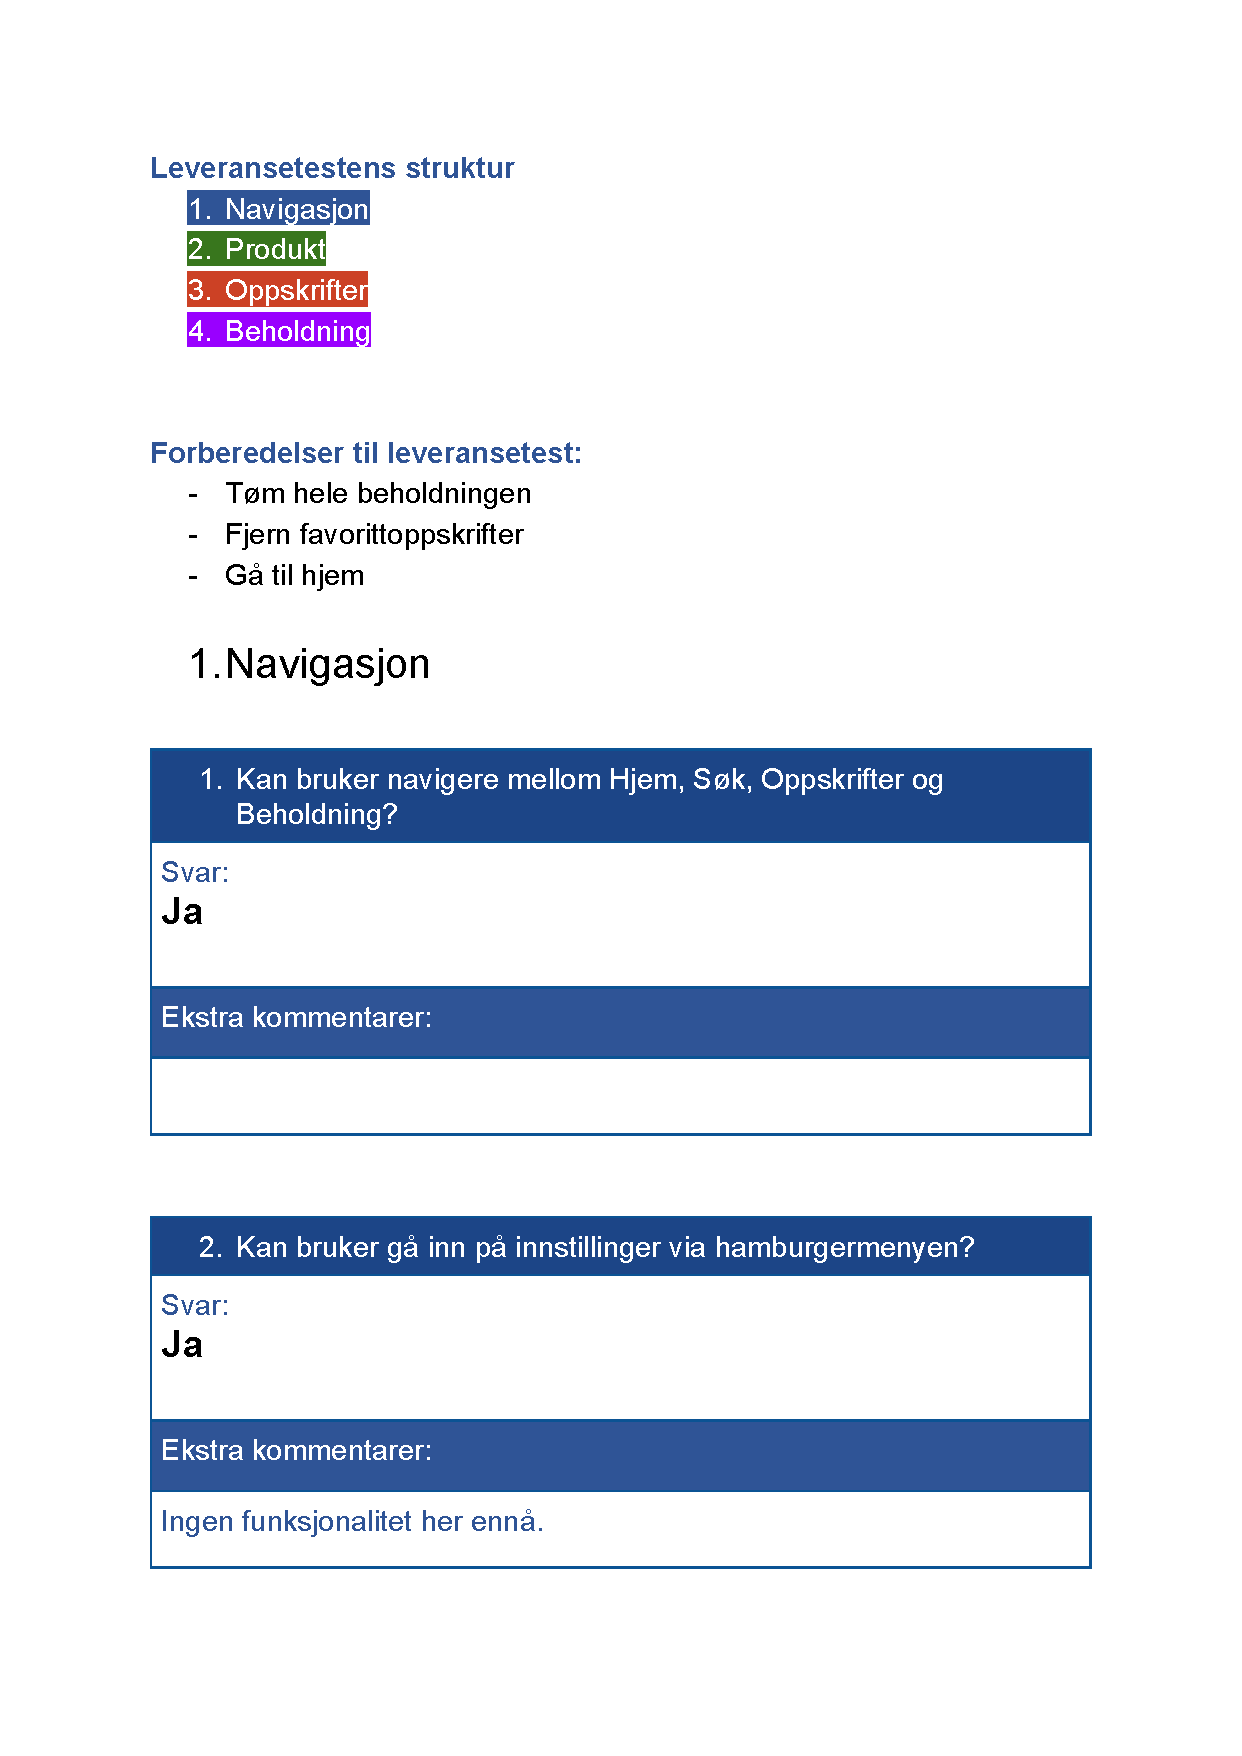
\includepdf[pages=-]{figures/vedlegg/Leveransetest}
%\chapter{Vurdering}
I dette avsluttende kapittelet skal vi drøfte og vurdere vår innsats

\section{\textbf{Vurdering av arbeidsmetodikk}}
\newthought{Å bruke en variant av SCRUM} som arbeidsmetodikk har vært til stor hjelp for oss underveis i prosjektet. Siden man kan bruke SCRUM som et rammeverk og velge eller luke bort deler av metodikken kan man skreddersy arbeidsmetodikk som passer teamet. I vårt tilfelle har det å kunne inkludere oppdragsgiver underveis i prosessen via sprintpresentasjoner vært svært viktig, mens daglig standup kanskje ikke alltid har vært like viktig siden vi har jobbet så tett store deler av prosjektet. Muligheten til å raskt omstille seg til nye situasjoner er kanskje bærebjelken til smidig metodikk og som vi nevnte i (KAP 8 REFERANSE) fikk vi smake dette på alvor i den dramatiske situasjonen som utspilte seg i forbindelse med virusutbruddet av Covid-19. 

Samtidig medfører en slik arbeidsmetodikk ekstra møter og tid i forbindelse med planlegging, presentasjoner og lignende. En utfordring med dette er kanskje motivasjonen til å være forberedt og gjennomføre disse møtene. Det har derfor vært viktig for gruppen å kommunisere på en god måte slik at arbeidsmoralen forblir høy. 



%\chapter{Veien videre}

\section{\textbf{Teknisk løsning}} 
\newthought{Vi estimerer} at vi vil bruke 4 sprinter på å gjøre løsningen klar til handover, hvor Kolonial.no kan begynne implementasjon.


\textbf{2-4 sprinter:}
\\Videre ville vi gjennomført flere brukertester for å forsikre oss om at brukerne har faktisk ønsker funksjonaliteten vi utvikler. Vi ønsker f.eks. å finne en bedre løsning på å flytte varer mellom beholdningskategorier. Etter tilbakemeldinger fra brukertestene er det noe brukerne opplever som vanskelig, og vi vil derfor bruke tiden videre på å kvalitetssikre en bedre løsning på dette. Vi har heller ikke fått testet brukere over tid, altså om løsningen vår er lett nok å bruke til at bruker orker å fortsette å bruke den, eller om det blir for tungvint å vedlikeholde beholdningen sin. For å teste dette måtte vi ha satt opp brukertester som hadde gått over 1-2 uker. 

Kolonial har i dag en holdbarhetsgaranti på 7 dager, men enkelte varer har annen merking, som f.eks 3 dager holdbarhet. Vi ønsker å implementere funksjonalitet for å varsle bruker om varer som er i ferd med å gå ut på dato, samt foreslå oppskrifter til disse varene, slik at man unngår å kaste mat. Vi kan i dag hente ut holdbarhetsdato fra Kolonial.no sitt API, og implementasjonen vil derfor være rask men vi ønsker å sette av tid til brukertesting i tillegg. 

\textbf{5-7 sprinter:}
\\Etter 4 sprinter estimerer vi at vi vil være klare for en handover. Vi ville brukt resterende tid av sprintene til å skrive teknisk dokumentasjon, og beskrive sorteringsalgoritmene slik at overgangen fra vår løsning til deres egen app blir sømløs. Med tanke på at vi ikke kjenner til kodebasen til Kolonial, eller hvor mye ressurser de ville satt av til å implementere løsningen, kan vi ikke si hvor lang tid det hadde tatt utover vårt arbeid frem til handover.

\section{\textbf{Kommunikasjon}}
\newthought{Veien videre kommunikasjonsmessig} vil være å benytte prediktiv markedsføring for å sikre fremdrift i fasene og øke CLV hos hver enkelt bruker, gjennom Marketing 4.0 metoden. Her må aktiviteter og målinger fra lojalitetshjulene, kobles opp mot prediktive analysemodeller, for å sikre at hver bruker opplever kommunikasjonen som verdifull for seg og sine ønsker og behov. 

Marketing 4.0 er en tilnærming som kombinerer online og offline interaksjoner mellom bedrift og bruker, sammen med Marketing 3.0. Målet med Marketing 4.0 er å drive brukere fra kjennskap til disippel (Kotler, m.fl. 2017, 66). Marketing 3.0 handler om å identifisere brukers ønsker og behov, såkalt verdibasert markedsføring (Kotler m.fl. 2010, 39). 

Marketing 4.0 benytter maskinlæring og kunstig intelligens for å forbedre produktiviteten av markedsføringen, samtidig som det fokuserer på det menneskelige for å styrke brukerengasjement (Kotler m.fl. 2017, 46-47). Dette er en del av prediktiv markedsføring, hvor klynging er en av de vanligste metodene for å øke CLV, og optimalisere kundeengasjementet. 

Klynging er en automatisk og statistisk prosess basert på algoritmer. Algoritmene analyserer hundrevis av brukerdata samtidig, og gir innsikt i hva som trigger de forskjellige handlingene til bruker. Dette er en motsetning til segmentering, som baseres på én eller to faktorer. Klyngene settes sammen på mest hensiktsmessig måte for å oppnå konverteringer, basert på hvilke produkter eller tjenester det er mest sannsynlig at bruker er interessert i å kjøpe eller interagere med (Artun og Levin 2015, 24- 26). 

Brukerinteraksjonen gjennom kanalmiksen og digitalisering har gjort det mulig å samle inn enorme mengder data om brukerne, ved at de selv legger inn sine preferanser og demografi, som kan brukes til personifisering av markedsføringen. Gjennom et kundeforhold vil denne informasjonen bli mer og mer detaljert, etterhvert som bruker legger igjen flere spor (Artun og Levin 2015, 10). 

Prediktiv markedsføring bruker prediktive analysemetoder for å kunne levere relevant og personlig budskap til bruker, ved alle berøringspunkter, gjennom hele kundeforholdet (Artun og Levin 2015, 3). Med prediktiv markedsføring og analyse er det ingen grenser på hvor mange kampanjer man kan utforme. Disse kan man hele tiden endre og videreutvikle, basert på tall fra prediktive analyser, for å forbedre og personalisere innholdet og drive fremdrift i brukerfasene (Artun og Levin, 16-17).

Ved å benytte denne metoden vil Kolonial.no plassere de rette brukerne i passende klynger, hvor de kan tilpasse innholdet enda mer til mer detaljerte målgrupper. På grunn av den automatiserte, analytiske tilnærmingen vil klyngene alltid være oppdatert, slik at når brukere beveger seg videre i lojalitetshjulet vil de motta kommunikasjon basert på riktig fase. På denne måten vil brukere i mye større grad føle at de får verdi av innholdet de presenteres for, fordi det tilpasses basert på klyngene. Dette igjen bidrar til økt CLV gjennom hele lojalitetshjulet. 

% the back matter
\clearpage
\bibliography{references}
\nocite{*}
\addcontentsline{toc}{chapter}{Bibliografi}
\bibliographystyle{chicagoNew}
\chapter{Vedlegg}
\label{chap:vedlegg}
\begin{sloppypar}

\section{\textbf{Markedsføring}}
\subsection{\textbf{Vedlegg 1:} Digital Involvement Cycle analysemodell - persona 1}
\label{vedlegg:1}
\url{vedlegg/tabell-dic-1.pdf}

\subsection{\textbf{Vedlegg 2:} Digital Involvement Cycle analysemodell - persona 2}
\label{vedlegg:2}
\url{vedlegg/tabell-dic-2.pdf}

\section{\textbf{Brukertester}}
\subsection{\textbf{Vedlegg 3:} Brukertester}
\label{vedlegg:3}
\url{vedlegg/brukertester.pdf}

\section{\textbf{Prototyper}}
\subsection{\textbf{Prototyper}}
\subsection{\textbf{Vedlegg 4:} Prototype 1}
\url{vedlegg/prototype1.pdf}
\subsection{\textbf{Vedlegg 5:} Prototype 2}
\url{vedlegg/prototype2.pdf}
\subsection{\textbf{Vedlegg 6:} Prototype 3}
\url{vedlegg/prototype3.pdf}
\end{sloppypar}

\singlespacing




\end{document}